%%%%%%%%%%%%%%%%%%%%%%%%%%%%%%%%%%%%%%%%%%%%
%                 Preamble                 %
%%%%%%%%%%%%%%%%%%%%%%%%%%%%%%%%%%%%%%%%%%%%

% This LaTeX document uses Cameron's LaTeX template (or some form of it) which
% is ever-evolving.

% --- Requirements ---
%
% Packages from Ubuntu [required for]:
%     texlive-publishers [revtex4-1]
%     texlive-science [siunitx]

%\documentclass[a4paper]{article}
\documentclass[a4paper, 12pt, twoside]{report}
%\documentclass[
% aps,
% %prb,
% a4paper,
% showpacs,
% superscriptaddress,
% notitlepage,
% %longbibliography,
% nofootinbib,
% preprint % gives 12pt font
%]{revtex4-1}

% --- Macro dependencies ---
%\usepackage{xcolor} % Uncomment if not using bibliography links

% --- Common ---
\usepackage[left=3cm, right=3cm, top=2cm, bottom=3cm]{geometry}
% NOTE Changed l/r margins from 2cm to 3cm, so textwidth changed form 
% 169.988mm to 149.988mm
% For debugging use showframe
\usepackage{graphicx}
\usepackage{amsmath}
\usepackage{amsfonts}
\usepackage{siunitx}
\usepackage{setspace} % For line spacing
\usepackage{braket}
\usepackage{physics}

% --- More optional ---
\usepackage{tabularx} 
\usepackage{xpatch} % To patch the TOC
%\usepackage{caption} % Helps with subfigs
\usepackage{subcaption} % For subfigures
\usepackage{enumitem} % Originally to resume list
\usepackage{overpic} % Superimpose text on images
\usepackage{datetime} % For custom dates
\usepackage[T1]{fontenc} % Some fonts in some bibs...
\usepackage{amssymb}
\usepackage{import} % For importing pgfs with embedded pngs
\usepackage{layouts}
\usepackage{mathtools} % Originally for prescripts

% --- Page headings ---
\usepackage{fancyhdr}
\pagestyle{fancy}
\rhead{\thepage}
\lhead{\leftmark}
\setlength{\headheight}{1.2cm}
\cfoot{}

% Redefine the plain page style (for chapter pages)
\fancypagestyle{plain}{%
  \fancyhf{} % Empty header and footer
  \fancyhead[R]{\thepage}
  \renewcommand{\headrulewidth}{0pt}% Line at the header invisible
  \renewcommand{\footrulewidth}{0pt}% Line at the footer visible
}

% --- Custom colors --- 
\usepackage[dvipsnames]{xcolor}
% Using custom color palette
\definecolor{blue}{HTML}{699ABB}
\definecolor{purple}{HTML}{994f95}
\definecolor{grey}{HTML}{736e75}
\definecolor{gold}{HTML}{d2ab22}
\definecolor{pink}{HTML}{D73665}
\definecolor{deeppurple}{HTML}{312032}
\definecolor{Lorange}{HTML}{d36800}
\definecolor{Lgreen}{HTML}{009915}

% --- Bibliography ---
% Uses biblatex with biber. Don't include url, doi, isbn because we will use
% magic to insert the url as a hyperlink in the title ourselves

% Ubuntu: requires texlive-bibtex-extra
\usepackage[backend=biber,
						url=false,
						doi=false,
						isbn=false,
						eprint=false,
						giveninits=true,
            sortcites=true,
            sorting=none
						]{biblatex}

% This is the macro to do this. see SE:
% https://tex.stackexchange.com/quACestions/23832/biblatex-make-title-hyperlink-to-doi-url-if-available
% and 
% https://tex.stackexchange.com/questions/48400/ACbiblatex-make-title-hyperlink-to-dois-url-or-isbn
\newbibmacro{string+doi}[1]{%
  \iffieldundef{doi}{#1}{\href{http://dx.doi.org/\thefield{doi}}{#1}}}
\DeclareFieldFormat{title}{\usebibmacro{string+doi}{\mkbibemph{#1}}}
\DeclareFieldFormat[article]{title}{\usebibmacro{string+doi}{\mkbibquote{#1}}}

% Manually remove notes
\AtEveryBibitem{%
  \clearfield{note}%
	}

% Bib file
\addbibresource{bib.bib}

% --- Bibliography Links ---
% Use the "colorlinks" option version for words highlighted rather than having
% boxes. The "border" options in hypersetup correspond to colorlinks false.
% OR use "hidelinks" option to make the links invisible.
\usepackage[colorlinks]{hyperref}
\hypersetup{
  linkcolor=pink,
  %linkbordercolor=pink,
	citecolor=blue,
  %citebordercolor=blue,
	urlcolor=purple,
  %urlbordercolor=purple
}
% And this macro adds urls to titles in bib


% --- Tikz ---
% Have to load tikz after xcolor
\usepackage{tikz}
\usepackage{pgfplots} % For plotting
\usetikzlibrary{calc,patterns,angles,quotes}

% --- Bib title (not line) ---
\def\bibsection{\chapter*{\refname}}

% --- Macros ---
%\newcommand{\diff}{\mathrm{d}} USE \dd (physics) instead
\newcommand{\cm}[1]{\textcolor{blue}{#1}} % For my comments
\newcommand{\mt}[1]{\textcolor{pink}{#1}} % For my comments
\newcommand{\ph}[1]{\textcolor{purple}{#1}} % Placeholders
%\renewcommand{\cm}[1]{} % Uncomment to remove my comments
%\renewcommand{\mt}[1]{} % Uncomment to remove markers for Mike's comments 
\newcommand{\incfig}[2]{\includegraphics[width=#1\textwidth]{#2}}
\newcommand{\myeqref}[1]{eqn~\eqref{#1}}
\newcommand{\mytabref}[1]{table~\ref{#1}}
\newcommand{\myeqrefs}{eqns}
\newcommand{\myfigref}[1]{Fig.~\ref{#1}}
\newcommand{\mytableref}[1]{Table~\ref{#1}}
\newcommand{\mysubfigref}[2]{Fig.~\hyperref[#1]{\ref{#1}~(#2)}}
\newcommand{\inlineref}[1]{Ref.~\cite{#1}}
\newcommand{\inlinerefs}[1]{Refs.~\cite{#1}}
\newcommand{\plane}[2]{$#1#2$\nobreakdash-plane}
\newcommand{\xyplane}{$x\,y$\nobreakdash-plane}
\newcommand{\pewpew}[2]{$\mathcal{L}^{#1}_{#2}$}
\usepackage{datetime} % TODO Why is this here?
\newcommand{\Alpha}{\mathrm{A}}
\newcommand{\mred}{\ensuremath{m_\text{red}}}

% Date with just the month and year (use `\monthyeardate\today`)
\newdateformat{monthyeardate}{\monthname[\THEMONTH] \THEYEAR}

% Chemicals
\newcommand{\CaF}{CaF}
\newcommand{\CO}{CO}
\newcommand{\YbF}{YbF}
\newcommand{\SrF}{SrF}
\newcommand{\Rb}{Rb}
\newcommand{\esRb}{\textsuperscript{87}Rb}
\newcommand{\efRb}{\textsuperscript{85}Rb}
\newcommand{\ottCs}{\textsuperscript{133}Cs}
\newcommand{\RbCs}{RbCs}
\newcommand{\SFsix}{SF\textsubscript{6}}
\newcommand{\He}{He}
\newcommand{\Ca}{Ca}
\newcommand{\AlN}{AlN}
\newcommand{\hiresSi}{HiRes Si}

% --- Units ---
% Custom units
\DeclareSIUnit\gauss{G}
\DeclareSIUnit\inch{inch}
\DeclareSIUnit\rpm{rpm}
\DeclareSIUnit\debye{D}
\DeclareSIUnit{\belmilliwatt}{Bm}
\DeclareSIUnit{\dbm}{\deci\belmilliwatt}
\DeclareSIUnit{\theohm}{ohm} % For spelling out 'ohm' in mw chapter
\sisetup{range-phrase=--}

% --- Line spacing ---
\onehalfspacing
\raggedbottom

% --- Table of contents ---
% Patch TOC to exclude *-ed sections (default behaivour in most classes, but
% changed by design in revtex). Also exclude (sub)subsections
% Patch is quite specific to revtex
\makeatletter
%\def\l@subsection#1#2{} % Uncomment to exclude subsection
%\def\l@subsubsection#1#2{} % Uncomment to exclude subsubsection
\patchcmd{\@ssect@ltx}
    {\addcontentsline{toc}{#1}{\protect\numberline{}#8}}
    {}
    {}
    {}
\makeatother

% --- Other macros ---
% Measured value
\newcommand*\meas[1]{\tilde{#1}}


% Uncomment and fill if using article
%\title{Early stage assessment: molecule chip}
%\author{Cameron McGarry\\ 
%Supervisors: Mike Tarbutt and Ben Sauer}

%%%%%%%%%%%%%%%%%%%%%%%%%%%%%%%%%%%%%%%%%%%%
%   Begin Document and Title/ Abstract     %
%%%%%%%%%%%%%%%%%%%%%%%%%%%%%%%%%%%%%%%%%%%%

\begin{document}

% Title page
\pagenumbering{gobble}
\begin{titlepage}


%  \begin{figure}
%    \includegraphics[width=70mm]{./figs/imperial.pdf}
%  \end{figure}

\begin{minipage}{14cm}
  \begin{flushleft}
    \vspace*{4cm}
    \rule{\linewidth}{0.5mm} \\[0.4cm]
    % Thesis: 
    %   (A) chip trap for CaF molecules
    %   Trapping of CaF molecules in a microfabricated magnetic trap
    %   (Something with microwaves?? -- unlikely I will get here anyway...)
    {\huge \bfseries Design and fabrication of a chip trap for \CaF{} molecules}\\
    \rule{\linewidth}{0.5mm} \\[1.0cm]
    \newgeometry{textwidth=11cm}
    {\large \textbf{Cameron McGarry}} \\[1.0cm]
    {\setstretch{1.2}
    \thesis{
    A thesis submitted to \\
    {\large \textsc{Imperial College London}} \\
    {\large \textsc{Department of Physics}} \\
    in partial fulfillment of the requirements for the degree of Doctor of
    Philosophy. \\[5mm]
    }
    Supervised by Mike Tarbutt and Ben Sauer \\[5mm]
    \makeatletter
    \monthyeardate\today
    \makeatother
    \restoregeometry
    }
  \end{flushleft}
\end{minipage}

\end{titlepage}


%% Abstract
%\chapter*{Abstract}
%\cm{TODO}

%% ESA Abstract (bits)
%Quantum optical systems are promising candidates for use in a vast range of
%technologies, from metrology, to simulation, to probing the fundamentals of
%physics. But despite their high controllability and coherence times, they often
%lack scalability, requiring ungainly optical systems to function.
%
%Chip traps were introduced as a means of miniaturizing such systems. Magnetic
%traps have been formed from fields generated by wires on a substrate and
%external bias fields. This forms a robust trapping environment with very high
%field gradients. Chips are innately scalable due to their fabrication by
%well-understood standard photolithographic methods, and have been routinely
%used for experiments with atoms. Atom chips have proven to be particularly
%useful in formation of Bose-Einstein condensates. They show promise for
%coherent control, and integration with other quantum systems via coupling to
%microwave guides also integrated with the chip.
%
%With the development of new technologies for the creation of ultra-cold
%molecules, realisation of a molecule chip is now a possibility. Rotational
%states of molecules couple strongly to microwave fields, allowing the
%exploitation of cavity QED effects for use in a scalable system which can be
%integrated with other quantum architectures.
%
%% LSR Abstatract
%In this report, we present ongoing work into development of a molecule chip
%operating on a magnetically insensitive transition of \CaF{}. In particular, we
%discuss simulations that have allowed us to refine the design of the chip
%trap, and the microfabrication techniques used to build a prototype chip.
%
%Simulations of the trajectories of molecules in magnetic traps have been
%performed. These are used to analyse the trap design, and to ensure that
%loading of molecules is possible through a series of adiabatic transfers
%between magnetic potentials. The phase space acceptance of traps is presented.
%
%The microfabrication of an earlier trap design is presented. Through-mask
%electroplating has been used to construct a chip with trapping wires with
%heights of \SI{3}{\micro\meter}. This is much taller than would be possible
%with conventional photolithography methods, and will allow for high currents to
%be carried on chip, thus forming deep magnetic traps for our molecules.

%\clearpage
%
%\chapter*{Declarations}
%I declare that all the work presented in this thesis is my own. Where the work
of others has been used it has been correctly and clearly attributed and
referenced.

The copyright of this thesis rests with the author. Unless otherwise indicated,
its contents are licensed under a
\href{https://creativecommons.org/licenses/by-nc-sa/4.0/}{Creative Commons
Attribution-NonCommercial-ShareAlike 4.0 International Licence} (CC BY NC-SA).

Under this licence, you may copy and redistribute the material in any medium or
format. You may also create and distribute modified versions of the work. This
is on the condition that; you credit the author, do not use it for commercial
purposes and share any derivative works under the same licence.

When reusing or sharing this work, ensure you make the licence terms clear to
others by naming the licence and linking to the licence text. Where a work has
been adapted, you should indicate that the work has been changed and describe
those changes.

Please seek permission from the copyright holder for uses of this work that are
not included in this licence or permitted under UK Copyright Law.


%\clearpage
%
% TODO Remove this chapter before submission to Spiral
%\chapter*{Covid-19 impact statement}
%This impact statement is included as part of Imperial College London's policy
on studies affected by the coronavirus pandemic. It will be removed after
examination, and will not feature in the final version of this thesis.

In this thesis I will describe the creation of a microfabricated chip trap for
laser-cooled \CaF{} molecules. The original intention was to design and build
such a device, and incorporate it into the existing \CaF{} experiment that we
operatre in the Centre for Cold Matter at Imperial College.

In March 2020 I was focusing on the fabrication of the
chip trap (described in chapter~\ref{fab}), which took place in the cleanroom
facilities at the London Centre for Nanotechnology. These were closed to
external users from 19\textsuperscript{th} March -- 1\textsuperscript{st}
October, completely halting development of this key aspect of the project. When
access resumed it was limited due to the requirement to social distance. This
meant that developing the fabrication procedure for the chip was severely
delayed.

The chip experiment has been designed to integrate with the existing \CaF{}
experiment (described in chapter~\ref{overview}) however the development of
this machine was delayed by the closure of the College laboratories starting on
18\textsuperscript{th} March. Since the existing experiments were not
sufficiently developed, and priority was given to other experiments using the
same apparatus, it was impossible to install the chip chamber. 

The combined result of these two effects was that the molecule chip experiment
was not fully implemented, and we were limited to the preliminary experiments
which are reported in chapter~\ref{exper}. The fabrication was completed, but
only to the point of implementing a single-layer trapping chip, without
integrated microwave guides. During the lab closures, the simulations in
chapter~\ref{sim} were conducted, and the chip design was improved, but this
effort was not sufficient to fully mitigate these considerable delays.

%\clearpage
%
%\chapter*{Acknowledgements}
%%\thispagestyle{empty}
\begin{singlespace}
If I did one thing right during my PhD it was choosing my supervisors. Ben, you
are a font of infinite wisdom in the lab, and have tolerated my bush-league
attempts at lab work, and your help in navigating the realities of academic
life is hugely appreciated. Mike, you are an incredibly committed individual,
and the fact that you constantly made time for me despite your immensely busy
schedule has not gone amiss. Thank you in particular for reading and re-reading
this thesis.  I am enormously grateful to both of you for your patience and for
everything you have taught me.

To the other members of the Centre for Cold Matter, I also thank you for making
my time as a PhD student educational and enjoyable. I think that all of you
have at some point (in cases at many points) made time to teach and
help me.
%
Particular thanks goes to Bharath Srivathsan and Kyle Jarvis who worked
directly on the chip experiment with me, suffering many laborious hours in the
cleanroom, and showing me what's what in the lab.
%
The experiment would not exist without Jon Dyne and David Pitman from the CCM
workshop produced many of the parts for the experiment.
%
Gautam Kambhampati allowed me to hijack his experiment, and ensured that I took
regular coffee breaks to maximise lab and office productivity.
%
Steve Etienne and Vj Krishnan from LCN, and Amado Bautista-Salvador from
Hannover were of great help with the microfabrication.
%
I must of course mention Sanja Maricic and Miranda Toora, who have been
unendingly helpful with my various inane requests.

I am grateful to have a wide circle of people to complain to when things have
gone wrong. The bored gamers: Aniq, Cathy, Jason, Jay and Yuki, your
incessant chat kept me sane when locked indoors for weeks at a time. When we
were allowed outside I enjoyed many an evening chatting physics and
nonsense in the pub with my course-mates:
Alvise, George, Hailey, Oli, Sam, Sisi, Simon and Will. 
%
Similar services have been provided by Jamie, Jonny, Luke and Sam. It's sad
that we can't spend more time together, but it's always fabulous when we do. To
the other friends, from CCCBC, OURCs and elsewhere, I'm sorry that my choice of
enormous margins has meant that you didn't quite get squeezed onto this page.

The most welcome distraction from studying over the last four years has been
time spent on the river or nearby with coffee. I am grateful to the ladies and
coaches of Thames Rowing Club. You never stop impressing me, and I will miss
yelling at you; I will not miss regularly waking up before five o'clock in the
morning.

Susie, thank you for putting up with me. You always keep me on the right path
(figuratively speaking only) and tolerate my ceaseless rambling with enormous
grace. Your support is beyond measure and you are my favourite human.

Finally, to my parents: I can't ever thank you for everything you have given
me. I love you both.

\end{singlespace}


% TOC
\tableofcontents
\clearpage

% Numbers on
\pagenumbering{arabic}
%NOTE This must be manually set so that numbering starts on title page
\setcounter{page}{5} 

%%%%%%%%%%%%%%%%%%%%%%%%%%%%%%%%%%%%%%%%%%%%
%                Body Start                %
%%%%%%%%%%%%%%%%%%%%%%%%%%%%%%%%%%%%%%%%%%%%



\chapter{Introduction}
\label{intro}
%\ph{guff}

\section{Why a chip trap?}
Cold atoms and molecules systems are promising for the implementation of new
quantum technologies. They have been used for devices in fields of
measurement~\cite{PhysRevLett.120.103201}, simulation~\cite{Gross995} and testing of
fundamental physics~\cite{DeMille990}. However, one of the main disadvantages
when compared to, for example, superconductor~\cite{Wallraff2004} or pure
optical~\cite{Browne2017} systems is the lack of scalability and
miniaturization.~\cite{nielsenandchuang}

In 1995, Weinstein and Libbrecht proposed an experiment for
studying cold atoms in environments with extremely high magnetic
gradients.~\cite{PhysRevA.52.4004} These gradients can be obtained by using
microfabricated wires in combination with a biasing field to form a trap above
a surface. Not only does this lead to an interesting environment for studying
new physics, but it introduces miniaturization into the cold-atom
toolkit.~\cite{2011Ac} There is also potential for integration of atomic or
molecular systems on a chip with other chip-based quantum
systems.~\cite{2011Ac, Kubo2011}

The first atomic chip trap was demonstrated four years later by Reichel et
al.~\cite{Reichel1999}. Their chip trap was shown to be a robust environment for
atomic experiments. The field of atom chips has since expanded~\cite{2011Ac},
with use as an architecture for creation of Bose-Einstein condensates being of
particular interest to many physicists.~\cite{Ott2001}

Although laser cooling of atoms has been commonplace since the late
20\textsuperscript{th} century, cooling of molecules has taken longer to develop
due to their more complex internal energy structure. However, this same rich
energy structure and other features of the molecules could be exploited to
produce new interesting technologies.~\cite{Tarbutt2018} We are now able to
produce \CaF{} molecules cooled below the Doppler limit~\cite{Truppe2017},
coherently control the states of such molecules~\cite{Williams2018}
and load molecules into a tweezer array.~\cite{Anderegg2019} These developments
open the door to the realization of a molecule chip.

A proposal by Andr\'e et al. in 2006~\cite{Andre2006} suggested integrating an
electrostatic trap with a microwave resonator on a chip. A single trapped
molecule would experience a strong coupling between its rotational states and
photons in the resonator, which could be used for long-range coupling of
molecular qubits, coherent control and measurement. Coupling to other quantum
architectures via flying photon qubits may also be
possible.~\cite{PhysRevLett.92.063601}

% I would like to find a citation for this, but Mike has previously said (lit
% review email) that it isn't necessary.
Microwave transitions in atoms could have been suggested, however these are
magnetic dipole transitions between hyperfine states. The coupling from an
electric dipole transition between rotational states of a molecule is orders of
magnitude stronger. 

In the following subsection I will further discuss the field of laser cooling of
atoms and molecules. The rest of the report will focus on chip trapping, the
design of our molecule chip for \CaF{} and the outlook for the remainder of the
project.


\section{Atomic and molecular chip traps}
\cm{
 Take-away points:
   Magnetic trap
   How to get CPW on (Bohi)
   MTT + big U to load is viable
   Required PSD???
 }

At the time of the original molecule chip proposal~\cite{Andre2006}, atom chips
had been loaded using a MOT as a source~\cite{Reichel1999, Ott2001}, however a
molecule MOT had not yet been \cm{built (better word choice?)}, and there was no
credible source of loading a chip of this type.\footnote{Stark declerator
molecule chips would be developed shortly after~\cite{Meek2009}, but Andr\'e et
al. presented no method of loading their chip design with the required phase
space density.}  

As discussed above, the field of cold molecules has now developed significantly.
These developments have made the implementation of a molecule chip \cm{feasible
(better word choice?)}. In
this section, we will review the state of chip trapping, including work on atom
chips and these supporting technologies.

In developing the molecule chip, we have been able to draw upon the
well-developed field of atom chips to inform our design choices. Let us consider
three different aspects of chip design: trapping on the chip, loading into this
trap, manipulation of trapped atoms or molecules.
\cm{Here I define three key features, I should endeavour to address each of
them. Perhaps as separate (sub)sections. I may even want to introduce this more
explicity/ formally further above.}

The Andr\'e proposal~\cite{Andre2006} suggests the use of an electrostatic trap
to contain the molecules, however this is not the only option available. In
fact, magnetic trapping of atoms is much more widely explored~\cite{2011Ac},
and the discovery of magnetically insensitive transitions in \CaF{} makes this a
promising choice for a molecule chip. As such we will focus in this section on
magnetostatic trapping of atoms above a chip.

\subsection{Magnetic trapping}
\label{chiptraps:magentic}

\cm{TODO: theory of macroscopic, then feed into miiatrurising and hence the next
section}

\cm{Talk about IP s . QP and spin flip, including further discussion about
theory of spin flip (majorana) losses and how much we can get away with (to be
expanded on further below for Z wire/ dimple traps where we get really small.}

\subsection{Wire traps}
\label{chiptraps:wiretraps}

The basic principle of a magnetic wire trap is explained in Reichel et
al.~\cite{Reichel1999} As illustrated in \myfigref{chiptraps:fig:reicheltrap} a
field zero can be created from the magnetic field of a straight wire, carrying
current $I$, and an external bias field. This is a two-dimensional trap
\cm{2D?}, with a zero running parallel to the wire. The bias field's direction
must oppose the direction of the wire field. To form the zero at some height $h$
above the wire the bias field must completely cancel the wire field at that
point, so that \cm{Need to check B or B-tilde..}
%
\begin{equation}
  B = \frac{\mu_0 I}{2\pi h}.
\end{equation}
%
As with other magnetic traps, atoms (or molecules) can be optically pumped into
weak-field seeking states such that they favourably occupy the region surround
the trap minimum.~\cite{Metcalf1999}

\begin{figure}
  \includegraphics[width=0.75\textwidth]{./figs/chiptraps/reicheltrap.pdf}
  \caption{The combination of the magnetic field due to a straight wire and a
  constant bias are shown to produce a zero, forming a two-dimensional trap for
  weak field seekers. This is the basic principle underlying all magnetic wire
  traps. Reproduced from Reichel et al.~\cite{Reichel1999}
  }
  \label{chiptraps:fig:reicheltrap}
\end{figure}

\cm{I should have described QP/IP difference above}
Such a field will form a two-dimensional trap for weak-field seeking particles.
To achieve a three-dimensional trap, we can overlay an additional wire,
carrying a smaller current than the first such that there is now some component
of magnetic field along the axis of the original trap. Applying a bias along
this axial direction will re-introduce a field minimum, forming a three-dimensional
\emph{dimple trap} shown in \myfigref{chiptraps:fig:dimpletrap}.~\cite{2011Ac}
Since the trap centre is now in general a field minimum rather than a
zero, it is a Ioffe-Pritchard trap.

\begin{figure}
  \includegraphics[width=0.75\textwidth]{./figs/chiptraps/dimpletrap.png}
  \caption{The field of a straight wire trap (current $I_0$ is perturbed by a
  second wire carrying a current $I_1 \ll I_0 $ and accompanying bias
  ($B_{b,x}$). The resulting field forms a three-dimensional dimple trap.
  }
  \label{chiptraps:fig:dimpletrap}
\end{figure}


% Maths for the traps, freq. grad. etc.
The trapping field of the dimple trap close to the centre can be described in
terms of the usual Ioffe-Pritchard equation~\cite{Foot2005}
%
\begin{equation}
  \mathbf{B} = B_0 \begin{bmatrix} 1 \\ 0 \\0 \end{bmatrix}
               + B' \begin{bmatrix} 0 \\ -y \\ z \end{bmatrix}
               + \frac{B''}{2} \begin{bmatrix} 
                  x^2 - \frac{1}{2}(y^2 + z^2) \\
                  -xy \\
                  -xz
               \end{bmatrix},
\end{equation}
%
where we have chosen the origin to be the trap centre (not to be confused with
the centre of the dimple wires). In this case, the field gradient and curvature
are
%
\begin{equation}
  B' = \frac{\mu_0 I_0}{2\pi h^2}
\end{equation}
%
and
%
\begin{equation}
  B'' = \frac{\mu_0 I_1}{\pi h^3}
\end{equation}
%
respectively. The field at the trap centre is
%
\begin{equation}
  B_0 = \widetilde{B}_x + \frac{\mu_0 I_1}{2\pi h}
  \label{chiptraps:eqn:bias}
\end{equation}
%
where $\widetilde{B}_i$ represents the bias field applied in the $i$ direction.
The trap frequencies are given by
\begin{equation}
  \omega_x = \sqrt{\frac{\mu_m}{m}B''}
  \label{chiptraps:eqn:axisfreq}
\end{equation}
and
\begin{equation}
  \omega_\perp = \sqrt{\frac{\mu_m {B'}^2}{m B_0}}
  \label{chiptraps:eqn:transfreq}
\end{equation}
where $\mu_m$ is the magnetic moment of the trapped particle (for our \CaF{}
transitions $\mu_m \approx \mu_B$, the Bohr magneton), and we have taken $x$ to
be the axial direction (aligned with $I_0$).~\cite{2011Ac} We can estimate the
expected frequencies that we would expect to achieve based on the current and
trapping height.

\cm{I probably want to go through this in a lot more detail including the
maths. This is all in the notebook that Ed Hinds gave me to start with.} A
typical final\footnote{Greater intermediary trapping heights are used as part of
the loading procedure.} trapping height will be around \SI{10}{\micro\metre}.
This allows on-chip microwave fields to interact with trapped atoms without
introducing any energy shifts  or significant attractive force acting on the
molecule from the Casimir effect or Van der Waals force.\footnote{Trapping
beneath this height could allow investigation of these effects on a quantum
scale and is in itself a goal of atom chip
trapping.~\cite{PhysRevA.56.R3350}}~\cite{2011Ac}

\cm{Probably want to expand this similar to for height}
The current that can be achieved in the chip will be limited by thermal
properties of the final chip design as will be discussed in
section~\ref{experiment:multilayer}. Typical achievable currents are estimated
to be around \SI{60}{\milli\ampere}. 
Using \myeqref{chiptraps:eqn:transfreq} and
\myeqref{chiptraps:eqn:axisfreq} we can therefore anticipate trapping frequencies
for \CaF{} of
%
\begin{align}
  \omega_x &= \SI{5e4}{\radian \per \second} \\
  \omega_\perp &= \SI{1e5}{\radian \per \second}.
\end{align}
%
\cm{Need to check reasonable value for $B_0$}
Where we have assumed a minimum value of $B_0 = \SI{1}{\gauss}$ has been chosen.
These figures are in line with what we would normally expect from a wire
trap.~\cite{2011Ac}

The trap depth is well-approximated by the energy associated with the bias
field. For a trap at height \SI{10}{\micro\metre} this gives a typical trap
depth on the order of a few tens of millikelvin.~\cite{2011Ac}

Other variations on the wire trap are possible. Running two perturbing wires
across one axis (with currents $I_1$ and $I_2$) will form an H-trap, shown in
\myfigref{chiptraps:fig:trapvariations}. Here the minimum will exist between the
two perturbing wires. Note that depending on the relative signs of $I_1$ and
$I_2$ it is possible to form either a Ioffe-Pritchard (currents parallel) or a
quadrupole trap (currents anti-parallel). Approximations of these shapes can be
formed by bending a single wire to create the axial confinement, forming either
a Z-trap (Ioffe-Pritchard) or U-trap (quadrupole), both also shown in
\myfigref{chiptraps:fig:trapvariations}. \cm{I should really show the fields
that are generated, as well as the bias fields required, a coordinate system and
follow up on expected Majorana losses properly below.}

\begin{figure}
  \centering
\begin{tikzpicture}
  % H
  \draw[thick, ->] (-6,0) -- (-3,0);
  \node at (-2.75,-0.25) {$I_0$};
  \draw[thick, ->] (-5.5,-3) -- (-5.5,3);
  \node at (-5.15, 3) {$I_1$};
  \draw[thick, ->] (-3.5,-3) -- (-3.5,3);
  \node at (-3.15, 3) {$I_2$};
  \node at (-6.5, -2.5) {(H)};
  % U
  \draw[thick, ->] (-1,3) -- (-1,0) --(1,0) -- (1,3);
  \node at (1.35,3) {$I$};
  \node at (-1.5, -2.5) {(U)};
  % Z
  \draw[thick, ->] (3,-3) -- (3,0) --(5,0) -- (5,3);
  \node at (5.35,3) {$I$};
  \node at (2.5, -2.5) {(Z)};
\end{tikzpicture}
  \caption{
    A top-down view of the wires forming an H, U and Z trap. The H trap has
    three independent currents, $I_0$, $I_1$ and $I_2$; usually the magnitudes
    of $I_1$ and $I_2$ will be the same, however their relative signs can be
    chosen to form either a quadrupole ($I_1 = -I_2$) or Ioffe-Pritchard ($I_1 =
    I_2$) trap. Note that these cases correspond to the U and Z wires
    approximating the currents through the H wire respectively. The bias fields
    requisite for trapping are not shown.
  }
  \label{chiptraps:fig:trapvariations}
\end{figure}

\cm{
``Frequencies for the other trap types can be calculated numerically, but the
above figures are presented as a representative example of what can be expected
from a wire trap.'' \\
%
Maybe I should actually do this and analyse these traps properly.
}

\subsection{Loading wire traps}

Reichel et al.~\cite{Reichel1999} were one of the first to demonstrate
mirror-MOT loading, where the surface of the chip is used as the mirror to from
a MOT close to the surface. The \esRb{} mirror-MOT held $5\times10^6$ atoms,
and was formed of four laser beams, with two reflected off the chip, making the
six beams in total that are required for trapping. The magnetic field is
generated by coils in anti-Helmholtz configuration, which are switched off in
favour of a large U-shaped wire, which provides a quadrupole field whose zero is
aligned with the chip. This is a very common scheme to bring atoms close to the
chip surface~\cite{Folman2000, PhysRevLett.97.200405, 2011Ac, Boehi2009},
however it has also been shown~\cite{0256-307X-25-9-034} that it is possible to
forego the coil MOT and load atoms directly from a MOT formed by a U-wire.
\cm{Figure of our CaF MOT?}

After establishing a mirror-MOT, Reichel et al. changed the bias field in order
to bring the cloud closer to the surface. They were then able to turn off the lasers
to achieve purely magnetic trapping, and transfer to the trapping wires on the
chip.
An adiabatic change of the bias fields was then used to
draw the atoms closer to the surface~\cite{Reichel1999, Folman2000}. This
principle can be exemplified by the straight wire trap, with
\myeqref{chiptraps:eqn:bias} showing that trapping closer to the wire requires a
higher bias field (or a lower current).

This principle can be extended to more complex trap types and varying the
currents through the trapping wires.~\cite{Folman2000} It is also possible to
construct a series of wire traps in close proximity, whose currents can then be
independently controlled such that the trap centre is moved between them. This
allows the use of higher currents through wide wires when the cloud is far from
the surface, but a smaller wire must be used when the atoms are close to it, so
that the approximation of an infinitesimally small wire remains accurate.

This adiabatic change of currents (through various wires) and bias fields is
another common step in the loading procedure~\cite{Folman2000,2011Ac,
RevModPhys.79.235} and can also be used to transport atoms above the
surface~\cite{Reichel1999, Schwindt2005}. Bringing the trap centre close to the
surface also compresses the atom cloud, and since the compressing force is
conservative~\cite{Metcalf1999}, this leads to adiabatic heating of the cloud.
Conservation of phase space density suggests that the final temperature will be
given by~\cite{Metcalf1999}
\cm{Check this cite is legit, and also follow up with this later. What are
trap temperatures going to be due to compression, etc.}
%
\begin{equation}
   T_1 = T_0\left(\frac{V_0}{V_1}\right)^\frac{2}{3}.
\end{equation}
\cm{Expand, need to have already established what trapping volumes we can expect
and $T_0$ so that we can give  a final temperature.}

\cm{Alex highlighted the "increasing number or atoms" think I need to figure out
something more specific to say about evaporative cooling and phase space
acceptance (expand the latter above?) (Talk about how the remaining atoms are
themalized so temp is reduced and differentiate forced evap cooling.)}
After compression, the likelihood of collisions between the atoms is increased,
which results in the loss of large numbers of atoms due to inelastic collisions.
The solution to this, as presented by B\"ohi et al.~\cite{Boehi2009} is to
evaporatively cool atoms in the larger traps, before transferring them into the
smaller traps. The magnetic traps are compressed to increase the collision
rates and then a radio frequency (RF) ramp is applied to remove the hottest
atoms from the trap, thus reducing the total energy and increasing the number of
atoms that will be accepted into the next (smaller) trap.~\cite{Foot2005,
Metcalf1999}

Also of note is the possibility of forming a MOT from a single laser beam using
a patterned wafer~\cite{Nshii2013}. This eliminates the need for multiple beams
to create a mirror-MOT. This has the benefit of offering a stable and highly
reproducible MOT for loading.

Direct loading of a chip with an optical tweezer is also a possibility for
transferring molecules directly onto a chip~\cite{Liueaar7797}, with Bernon et
al.~\cite{Bernon2013} having demonstrated the technique with atoms. In this
experiment, an optical tweezer transported a cloud of $5\times10^6$ \esRb{}
atoms from a MOT onto a chip trap \SI{40}{\milli\metre} away. This has the
benefit of insignificant losses and heating. This is a very attractive option
for loading, but molecular optical tweezers are still in their
infancy~\cite{Anderegg2019}, so this is left as a possibility for future
research. \cm{Need to check this later.}

\cm{Should expand this paragraph into a whole section.}
%
Fabrication of atom chips makes use of standard photolithographic procedures to
create wires that form traps.~\cite{2011Ac}. However, this is an inefficient way
to create wires of the desired height (usually several micrometres, whereas
photolithography produces structures tens of nanometres tall). This prevents the
formation of traps high above the surface. In order to achieve the required
heights, it is possible to first lay down a seed layer of gold and then create a
mould made of photoresist in the shape of the desired wires. Electroplating can
then be used to build up the wires before cleaning off the mould and etching off
the seed layer.~\cite{4797887} \cm{Maybe I should point this at the
fabrication section. DOn't know if I need a brief summary here...}

\subsection{Molecule chips}
\label{chiptraps:molculechips}


Molecule chips that have been previously implemented utilise different loading
schemes to those discussed for atom chips. In 2008 Meek et al.~\cite{Meek2008}
have loaded \CO{} molecules directly from a supersonic beam, with on-chip
slowing performed by a Stark decelerator integrated into the chip.

Fabrication of a chip-based Stark decelerators using photolithographic
techniques is significantly less involved than construction of a macroscopic
decelerator, providing excellent scalability; Meek et al. used over 1200
electrodes, as opposed to the 63 stages used in an equivalent macroscopic
experiment~\cite{Bethlem1999}. The electric field above the surface of the chip
was varied to slow of molecules from a \SI{312}{\metre\per\second} beam to a
standstill, constraining them \SI{25}{\micro\metre} above the surface in
tube-shaped clouds, \SI{20}{\micro\metre} in diameter.~\cite{Meek2009}

On-chip control of the molecules was demonstrated by the same group, using
microwaves propagating through free space~\cite{doi:10.1002/cphc.201001007} and
separately with infrared light~\cite{doi:10.1080/00268976.2012.683885}.  \CO{}
molecules in the $J=1$ rotational state were rotationally excited into the $J=2$
state on the chip, then accelerated off chip for state-selective detection.
On-chip imaging has since been achieved, but has not been fully integrated with
the chip, still requiring external optics.~\cite{Marx2013}

Whilst being a clear demonstration of the potential of
molecule chips, the lack of on-chip measurement and integrated control mean that
these chips are inherently not scalable.  Furthermore, the trapping volumes were
still fairly large, around \SI{0.25}{\milli\metre\cubed}. 
%
\cm{Why do we want a small trap volume?}

\cm{PSD of beam? Why did Mike say this was no good for us?}
%
The use of on-chip decelerators was motivated by a lack of laser-cooled
molecules, however this has now been achieved, producing sources of high
phase-space densities~\cite{Truppe2017}, which could be used for loading a
different design of chip such as that proposed by Andr\'e et
al.~\cite{Andre2006}

\cm{Alex: explain further how coupling can create qubit and do sideband
cooling.}
%Sideband cooling I think is more to do with increased coupling than whatever
%nonsense I came up with in viva. So can't do in free space for some reason...
The Andr\'e proposal outlines an electrostatic trap for molecules embedded in a
microwave resonator to form a cavity-QED system. The high coupling between the
molecule and cavity photons could be used for forming a qubit and sideband
cooling into the ground state of the trap. The microwave guide can be used for
quantum control, and on-chip measurement by applying an off-resonant microwave
pulse. This design promises a robust trap with potential for integration with
other chip-based qubits (either other trapped molecules or different quantum
architectures).
\cm{what exactly is benefit of a resonator?}

\subsection{Quantum control on macroscopic and microscopic scales}
\label{chiptraps:control}

\cm{May want to think about moving this subsection to help with flow. Also
would be good to expand with some rigor/ theory.}

\cm{This next paragraph is very qualitative. I could expand it by
introducing Jayne's Cummings and going through the maths, but this is only
really useful if we can talk about it as a reasonable thing to try (i.e. if we
can do a superconducting chip).}
%
Coherent control of atomic and molecular states has been achieved in macroscopic
traps~\cite{Gross995, Blackmore_2018}, and is an essential tool for quantum
technologies. For example, the ability to address a single atom in an optical
lattice can be used to simulate other quantum systems such as a Mott
insulator.~\cite{Weitenberg2011} Coherent control of atoms on a chip has also
been achieved.~\cite{PhysRevLett.92.063601} Of most relevance to this report is
the experiment by B\"ohi et al.~\cite{Boehi2009} who observed Ramsey fringes on
the hyperfine levels of \esRb{} using microwaves carried across the surface of a
chip. Coherent control achieved in this manner is innately robust and scalable;
and therefore highly desirable for applications in quantum technologies.
\cm{Alex: why is it innately robust and scalable?}

\cm{Need more legit version of this paragraph. For one thing I should be
able to calculate the lifetime (and hence Q factor) that I need.}
%
In order to achieve strong coupling between the trapped atoms (or molecules) and
the microwaves there must be good overlap between the microwave field and the
cloud.  If the trapped particles experience different field intensity or
polarization across the trap then this will affect the fidelity of any
operations.~\cite{Williams2018} If a microwave resonator is used then it must
have a lifetime long enough to sustain the interaction between the field and the
molecules during any pulse. This has been achieved in atoms for quality factor
$Q\sim2200$.~\cite{Hattermann2017}

\cm{Is ``qubits'' the right thing to refer to here?}
%
For molecules, it is possible to use microwaves to control the rotational
states~\cite{Blackmore_2018}, which do not exist in atoms. This results in a
coupling between the microwaves and the particles, which is orders of magnitude
stronger for molecules. The Andr\'e proposal~\cite{Andre2006} suggests that this
could be exploited to allow long-range coupling to other qubits, or sideband
cooling into the trap ground state.

\cm{This paragraph will need updating with cites for the 40GHz paper when
released. Should probably expand.}
%
Recently, magnetically insensitive transitions have been discovered in
\CaF{}.~\cite{Williams2018, Blackmore_2018}  One transition between
the $\ket{N=0, F=1, M_F=1}$ and $\ket{1,2,2}$ states has been found at
\SI{20.5}{\giga\hertz} and another between $\ket{1,2,2}$ and $\ket{2,3,3}$ at
\SI{41}{\giga\hertz} . The \SI{20.5}{\giga\hertz} transition has been shown to
be highly insensitive to the magnetic field ($\dd f / \dd B =
-\SI{105(4)}{\hertz\per\gauss}$). This makes it a promising target for a qubit
transition, as long coherence times of up to \SI{0.61(3)}{\milli\second} have
been observed~\cite{Blackmore_2018}. In as yet unpublished work, the
higher-frequnecy transition has been shown to be even more insensitive ($\dd f /
\dd B = -\SI{4.6(1)}{\hertz\per\gauss}$). 

This makes the $\ket{1,2,2} \leftrightarrow \ket{2,3,3}$  transition in \CaF{} a
promising candidate for quantum control in a magnetic chip trap. The need for an
electrostatic trap is removed by the magnetically insensitive transitions and
the existing atom chip technologies such as those created by B\"ohi et
al.~\cite{Boehi2009} provide a blueprint for implementation.


\section{Production of cold \CaF{} molecules}
\ph{A summary of our experiments, basically Hannah's thesis, Rb/CaF experiment
and transport coils. Also reference other similar experiments}
\cm{It might make sense for this section to become a chapter of its own right.}

\subsection{Laser cooling of atoms}

A brief discussion of laser cooling is presented here. More detailed discussion
can be found in references~\cite{Metcalf1999,RevModPhys.70.721,McCarron_2018}.

The basic principle of laser cooling of atoms is to deflect atoms from their
trajectory by transfer of momentum from the laser light (radiation
pressure).~\cite{RevModPhys.70.721} Consider a moving atom with a
pre-chosen cooling transition between two internal states.  When such an atom
encounters a counter-propagating resonant photon, absorption can take place,
reducing the atom's momentum. The atom can re-emit the photon in any direction,
but on average the resulting atom will be slower than before the encounter.
This process is known as Doppler cooling, as the light must be detuned from
resonance to account for the Doppler shift experienced by the moving
molecule.~\cite{Metcalf1999}

Of course, the assumption of a two-level system is a simplification. A key
example is sodium, where the transition $3S_{1/2}\, (F=2) \rightarrow 3P_{3/2}\,
(F'=3)$ was used to demonstrate this technique. However, since the excited
states of sodium have decay channels into $F=1$, it is possible for atoms to
fall into this state and out of resonance with the cooling
transition.\footnote{To be precise, $F'=3$ has no decay channels to $F=1$, but
off-resonant excitation into $F'=2$ can result in the population of dark states
by the decay $F'=2 \rightarrow F=1$. The repump operates on $F=1\rightarrow
F'=2$.} This can be overcome by introducing repumping light to transfer atoms in
dark states back into bright states.~\cite{RevModPhys.70.721} \cm{figure?}

We will foucs on atomic sources that produce a beam, with typical velocities of
a few \SI{100}{\metre\per\second}.~\cite{Metcalf1999}  As the atoms are slowed,
the Doppler shift they experience will change, and hence they will move out of
resonance with the transition.~\cite{RevModPhys.70.721} This can be overcome by
introducing chirped light, so that the frequency of the cooling light varies
across the lenght of the beam.~\cite{Prodan1984} In contrast, the Zeeman slower
applies a varying magnetic field. to shift the transition frequency of atoms
along the beam while the frequency of the light is kept the same.

An optical molasses can be formed from a pair of counter-propagating laser
beams, both red-detuned from the cooling transition. This means that if an atom
moves towards either beam it will undergo Doppler cooling.  A set of three
perpendicular optical molasses can cool an atom in each direction, reducing the
temperature but not providing any trapping force~\cite{Metcalf1999} . Further
cooling can be achieved in an optical molasses by choosing the polarization of
the light such that there is a polarization gradient. This sub-Doppler cooling
allows atoms to be cooled to the lowest limit, the recoil temperature of the
atoms (typically a few microkelvin).~\cite{Dalibard:89}

Trapping can be achieved (for example) by optically pumping the atoms into a
weak-field seeking state and applying a magnetic field to form either a
quadrupole~\cite{PhysRevLett.54.2596} or
Ioffe-Pritchard~\cite{PhysRevLett.51.1336} trap. \cm{Magnetic trapping is
discussed further in section~\ref{chiptraps}.} Magnetically trapped atoms can be
further cooled by evaporation, which can ultimately be used to form a
Bose-Einstein condensate.~\cite{Anderson198} A quadrupole trap combined with an
optical molasses forms a magneto-optical trap (MOT) in which atoms are
simultaneously trapped by the magnetic field and cooled by the
lasers.~\cite{PhysRevLett.59.2631}

The MOT has become a fundamental component of many cold atom experiments, a vast
field which we cannot explore in any level of detail here. Of particular note to
us are experiments involving dipole trapping~\cite{PhysRevA.47.R4567}, such as
those in an optical lattice~\cite{Bakr2009} or tweezer~\cite{Ashkin:86}. Control
of the atomic states in a lattice has been used to precisely realise the
second~\cite{PhysRevLett.120.103201} and to perform quantum
simulation~\cite{Gross995}.

\subsection{Laser cooling of molecules}

The rich energy structure of molecules, having rotational and vibrational
degrees of freedom, makes cooling procedures more involved~\cite{Tarbutt2018,
1367-2630-17-1-015007}, but there are numerous properties of molecules that
could be exploited in a range of applications. The large electric dipole moment
of some diatomic molecules means that they interact more strongly with electric
fields than atoms, making an optical lattice of molecules, or a molecule on a
chip, a good candidate for scalable quantum simulation or
computing~\cite{Micheli2006, Andre2006}.  Collisions between cold molecules
could allow investigation of the nature of quantum chemistry~\cite{Krems2008},
and cooled \YbF{} is being developed to precisely measure the electron electric
dipole moment as a means of testing fundamental theories of
physics~\cite{Lim2018}.

The tools developed for creation of cold atoms can be directly applied to
producing cold molecules. A MOT of \esRb{} and \ottCs{} can be used to form
\RbCs{} via an interspecies Feshbach resonance~\cite{PhysRevA.85.032506,
PhysRevA.89.033604} and then transferred into the ro-vibrational ground state by
stimulated Raman adiabatic passage.~\cite{PhysRevLett.113.255301,
RevModPhys.70.1003}.

Direct laser cooling of molecules can be challenging due to the complex energy
structure. The presence of numerous decay channels means that many repumping
beams can be required to keep molecules in bright states. One way to avoid use
of lasers is to slow molecular beams with a Stark decelerator, which removes
energy from dipolar molecules by varying an electric field across the
beam.~\cite{Bethlem1999} However the energy structure of some molecules makes
them good candidates for laser cooling.~\cite{Shuman2010,}
\cm{I want to find a good cite here that lists candidate molecules for laser
slowing...}

\cm{Should I mention dual-frequency or rf mots?} Beams of \SrF{} and \CaF{} have
been slowed with chirped light~\cite{PhysRevLett.108.103002, Truppe2017a} and
held in a MOT~\cite{Barry2014, Williams2017}. Sub-Doppler
cooling~\cite{Truppe2017} and coherent control of the rotational state have been
demonstrated for \CaF{}.~\cite{Williams2018, Blackmore_2018} \cm{And also for
other mols?} Early experiments with optical tweezers have also been
performed.~\cite{Anderegg2019}

\cm{Will need to re-visit these last two paras as these experiments will
have progressed. Also can probably sort cites}

Ongoing experiments with \CaF{} aim to achieve an increased phase space density by
sympathetic cooling with \esRb{} in a dipole trap.~ Recent
work has also discovered two vibrational transitions which are highly
insensitive to a magnetic field, making them ideal candidates for a qubit
transition in a molecule chip.


\section{An outline for a \CaF{} chip trap}
\ph{A cloud of cold molecules will be produced by the source described
above...}

The cloud will then be transferred into a magnetic transport trap (MTT) formed of
a pair of anti-Helmholtz coils external to the chambers. The dipole trap will be
switched off and the current in the coils ramped up to form a quadrupole trap.
The coils are mounted on a transport stage, such that they and hence the centre
of the quadrupole, can be moved across to neighbouring chambers. The trapped
cloud of \CaF{} and \esRb{} will be transported in the magnetic trap.
The MTT has been designed for loading into a neighbouring tweezer experiment,
however this will be extended to allow loading onto the chip. The MOT, MTT and
tweezer experiment are shown in \myfigref{experiment:fig:MTTsetup}. 

\begin{figure}[ht]
  \includegraphics[width=0.8\textwidth]{./figs/existing_chambers.png}
  \caption{
    \cm{Need to do a proper CAD for my chamber.}
    The MOT and tweezer chambers for existing experiments. The magnetic
    transport trap (MTT) is used made up of a pair of transport coils arranged
    in anti-Helmholtz configuration. These generate a quadrupole field, which
    will move with the coils on a translation stage, allowing the transfer of
    molecules trapped in the MOT chamber into the tweezer chamber. The chip
    chamber will be positioned further downstream (left) of the tweezer chamber.
    This CAD was undertaken by Kyle Jarvis.
  }
  \label{experiment:fig:MTTsetup}
\end{figure}

The chip flange will be mounted in a third chamber downstream from the MOT and
tweezer chambers. The flange is to be aligned such that the cloud can pass above
the surface with good clearance, entering on the side of the holding chip opposite
the flange. A macroscopic trap, aligned with the centre of the MTT, can then be
generated by the onboard U-wire and surrounding bias coils. This intermediary
trapping stage will be used to align the cloud with those on the science chip.

The cloud can be brought closer to the surface of the chip by a series of
current ramps in the bias coils and chip wires. By adiabatically changing the
bias fields and currents it is possible to transform the trapping potential
without ever distorting it to the point that it is no longer a trap.

A ramp is performed by linearly changing the trapping currents (those in the
Z-wires and bias coils). The time over which a ramp should occur is expected to
be on the order of tens of microseconds, so that the molecules experience an
adiabatic change of the potential.~\cite{Boehi2009} The proposed series of
trapping stages for loading into the dimple is shown in
\mytabref{experiment:table:loading}, along with required trapping currents and
bias fields.

\cm{Temperature/ compression? Proportion of molecules we expect to be able
to keep? Also just realy need to review this. Often don't need an x bias and
$B_0$ is basically always zero. Also qudrupole trap depth.}



\section{The structure of this thesis}
\ph{TODO, LAST!!}


\chapter{Background theory}
\label{theory}
%This chapter outlines some backtround theory that will be important throughout
the rest of the thesis. In section~\ref{theroy:cool} I will give an abstracted
overview of the principles of laser-cooling and trapping of atoms and
molecules, including magnetic traps. In section~\ref{theory:chips} I will
explain how it is possible to create magnetic fields for such traps using wires
on the surface of a chip. Finally, I will introduce the structure of diatomic
molecules, which is essential for applying these techniques in our experiment.

\section{Laser-cooling and trapping}

\subsection{Doppler cooling}

We will introduce Doppler cooling in the idealised case of a two-level atom or
molecule (henceforth the particle) travelling in one dimension, $x$.  Say that
light is incident on the particle from the positive $x$ direction. If the light
is resonant with an internal transition then the particle can absorb a photon,
which will at some later time be re-emitted the particle decays. The
emission of the photon has no preferred direction, and so over a large number
of these scatters the average effect is a net reduciton in the atom's velocity
in the positive $x$ direction.

In order to quantify this process, we might start by asking ourselves, what is
the force exerted on the particle by the photons? This will be~\cite{Foot2005}
%
\begin{equation}
  F = \text{photon momentum} \times \text{scattering rate}.
\end{equation}
%
The photon momentum is the usual value
%
\begin{equation}
  p_\gamma = \hbar k = \frac{hc}{\omega}
\end{equation}
%
and the scattering rate will be the product of the decay rate of the transition
(its linewidth) $\Gamma$ and the population of the excited state $\rho_{22}$.
We write the excited state in this way since it can be found from the optical
Bloch equations in the rotating wave approximation and in steady state to
be~\cite{Metcalf1999}
%
\begin{equation}
\rho_{22} = \frac{\Omega^2/4}{(\omega-\omega_0)^2 + \Omega^2/2 + \Gamma^2/4}.
\end{equation}
%
Where $\Omega$ is the Rabi frequency. We introudce the unitless parameters
$\delta = (\omega - \omega_0)/\Gamma$ and $s=\Omega^2/(2\Gamma)$ so that
%
\begin{equation}
  \rho_{22} = \frac{s/2}{\delta^2 + 1 + s}.
\end{equation}
%
We can now write down the scattering rate
%
\begin{equation}
  R = \frac{s\gamma}{\delta^2 + 1 + s}
\end{equation}
%
and force follows as
%
\begin{equation}
  F = \frac{s\gamma}{\delta^2 + 1 + s}\hbar k.
\end{equation}

The force acting on the particle can be related to its velocity by the Doppler
effect. A particle moving at speed $v$ will have its resonant frequency shifted
so that it has some new frequency $\omega'$ such that
%
\begin{equation}
  \frac{\omega'-\omega_0}{\omega_0} = \frac{v}{c},
\end{equation}
%
i.e.\ the frequency is red-detuned from the transition frequency at rest. The
result is that $\delta$ can be re-written as
%
\begin{equation}
  \delta \rightarrow \delta_+ = \delta + \frac{\omega_0}{\gamma c}v
\end{equation}
%
where $\delta$ represents the detuning of the laser from the resonant frequency
at rest, and the second term is the additional shift due to the Doppler effect.

However, what if the light is incident from the negative $x$ direction? In this
case, there is a blue shift, and we have
%
\begin{equation}
  \delta \rightarrow \delta_- = \delta - \frac{\omega_0}{\gamma c}v.
\end{equation}
%
By combining counter-propagating beams, it is possible to create a net force
%
\begin{equation}
  F_\text{res} = F_+ + F_-
\end{equation}
%
where
%
\begin{equation}
  F_\pm = \frac{s\gamma}{\delta_\pm^2 + 1 + s}\hbar k.
\end{equation}
%
For small $v$ we perform a Taylor expansion around $v=0$ to find that
%
\begin{equation}
  F_\text{res} \approx \frac{ s \delta}{(1 + s
  +\delta^2)^2}4\hbar k^2v.
\end{equation}
%
Which is maximised when $\delta = -1$ and $s = 1 + \delta^2 = 2$, so that
%
\begin{equation}
  F = - \alpha v
\end{equation}
%
where $\alpha  = - \hbar k^2 /2$.

So the counter-propagating beams provide a velocity-dependent damping
force. We call this arrangement an optical molasses, and it can equally be
applied in three dimensions.
%
It is important to note that the particles will not be brought to a standstill
under this effect. The molasses force does not contain the information
on the heating that occurs when the particles re-emit the absorbed photons.
This stochastic process limits the minimum attainable temperature to the
Doppler temperature~\cite{Metcalf1999}
%
\begin{equation}
  T_D = \frac{\hbar\Gamma}{k_B}.
\end{equation}

\subsection{Magneto-optical trap}

Doppler cooling is an important tool in the creation of ultracold atoms and
molecules, but it is of note that this technique does not provide any
position-dependent restoring force. In other words, particles that are slowed
by the above-described techniques are not trapped.
%
The magneto-optical trap (MOT) is the preeminent tool of atomic and molecular
physics, providing a way to trap a relatively cold gas of particles. It is the
backbone of many experiments including our own~\cite{Williams2017}. In this
section I will describe the basic operation of the common type-I MOT, that is a
two level system where the ground state has angular momentum $F$ and the
excited state has angular momentum $F'$ such that $F''>F$. In this example
$F=0$ and $F'=1$ are chosen.  In reality the molecule MOT that we will discuss
is a type-II MOT ($F'\leq F$) but such systems are more complicated and will be
discussed in the context of our experiment in section~\ref{section:overview}.

The MOT consists of two components, a magnetic quadrupole field, and restoring
laser beams, which are detuned from the $F\rightarrow F'$ transition by some
amount $\delta$. This setup is shown for one dimension in
\myfigref{theory:fig:MOT}. The Zeeman effect lifts the degeneracy of the excited state, and
introudces the usual energy shift~\cite{Binney}
%
\begin{equation}
  \Delta E = g_F m_F \mu_B B
  \label{theory:eqn:zeeman}
\end{equation}
%
where $g_F$ is the Land\'e g-factor, $\mu_B$ is the Bohr magneton, and $B$ is
the magnetic field. For a one-dimensional quadrupole field, we write $B=B'x$,
where $B'$ is the field gradient. We therefore have a position-dependent change
in the energy. Note that for negative $x$, the $m_F=-1$ state has lower energy,
and for positive $x$ the $m_F=1$ state has lower energy (when $g_F>0$, if
$g_F<0$ this is reversed).
%
The detuning $\delta$ is chosen such that this shift brings the lowered state
into resonance with the light. That the particle will then preferentially
absorb photons when it is away from the trap centre.

\begin{figure}[ht]
  \centering
  \includegraphics[width=0.8\textwidth]{figs/theory/motThesis.pdf}
  \caption{Illustration of the operating principle of a one-dimensional MOT on
    a two-level system with $F=0$ and $F'=1$. The particle is represented by
    the circle, and has counter-propagating beams of light (pink arrows)
    incident on it. A quardupole magnetic field is applied, lifting the
    degeneracy of the excited state as shown by the black lines. The light is
    red-detuned so as to be resonant with the transition to the lower $m_F$
    state, but only the restoring beam will be absorbed due to the choice of
    polarisation. The direction of the momentum change $\Delta\mathbf{p}$ is
    indicated by the black arrows. The excited state will decay back to the
    ground state (dashed lines).
  }
  \label{theory:fig:MOT}
\end{figure}

We wish to ensure that when a photon is absorbed the momentum change provides a
restoring force towards the centre of the MOT. This is achieved by choosing the
polarisation  so that the light coming from the positive (negative) direction
has $\sigma^+$ ($\sigma^-$) polarisation. The result is
that the particle will then always absorb light that is propagating towards the
centre of the trap, resulting in a restoring force. We also observe the same
Doppler cooling force from the molasses, so the resulting force is
%
\begin{equation}
  F = - \alpha v - \left(\frac{\mu_B B'}{\hbar k}\right)\alpha x.
\end{equation}

\subsection{Sub-Doppler cooling}

We might expect that a MOT would cool the atoms to around the Doppler
temperature, but in fact the temperate reached is often lower, due to
sub-Doppler cooling effects that often occur in a MOT. The most common of these
is polarisation gradient cooling, which cannot occur in the $F=0$, $F'=1$
system used to introduce the MOT. We instead consider a new system with
$F=1/2$, $F'=3/2$ which we note is still a type-I MOT.

In the centre of the MOT where there is near zero magnetic field, the $m_F$
states of the system would be degenerate expect that the degeneracy can be
lifted by the field of the light. This is the a.c. Stark shift, which is a
function of the light's polarisation. When the light has $\sigma_\pm$
polarisation, the $m_F=\mp1/2$ state is mixed more strongly with the exited
state, and so is higher. The relative matrix elements are shown in
\mysubfigref{theory:fig:subdoppler}{a}.

\begin{figure}[htb]
  \centering
  \begin{subfigure}[b]{0.45\textwidth}
    \begin{overpic}[width=0.8\textwidth]{figs/theory/pump.pdf}
      \put(4, 50){(a)}
    \end{overpic}
    \end{subfigure}
  \begin{subfigure}[b]{0.45\textwidth}
    \begin{overpic}[width=0.8\textwidth]{figs/theory/molasses.pdf}
      \put(4, 50){(b)}
      \put(105, 60){$F'=3/2$}
      \put(105, 28){$F=1/2$}
      \put(98, 2){Polarisation} % Was at x=105 but went outside hbox
    \end{overpic}
    \end{subfigure}
    \caption{In (a) we have the optical pumping scheme, and polarisation shift
      for $\sigma^+$ light. The relative coupling strengths (squared values
      shown inline) cause the $m_F=1/2$ state to be reduced further than
      $m_F=-1/2$.  The reverse is true for $\sigma^-$ light. The optical
      pumping (pink arrows and dashed decay) show how population can be
      transferred to $m_F=3/2$. A similar scheme can be used to pump to
      $m_F=-3/2$ with $\sigma^-$ light. Subfigure (b) shows the polarisation
      gradient cooling scheme described in the main text.  The polarisation
      gradient is depicted in the bottom row, and the $m_F=1/2$ ($m_F=-1/2$)
      state is shown by the dashed (solid) line. A particle in the molasses
      (pink circle) will follow a path such as the one shown here in pink,
      being pumped into the $F'=3/2$ state at the top of the potential hill,
      then decaying (dashed grey lines) back to the lower of the ground states
      and climbing the hill again.
  }
  \label{theory:fig:subdoppler}
\end{figure}

The counter-propagating beams establish a polarisation gradient across the
trap, and hence the Stark shift of the ground states also varies across the
trap, as shown in \mysubfigref{theory:fig:subdoppler}{b}. We have the additional effect that the
$m_F=\pm1/2$ state is only pumped by the $\sigma^\mp$ light, and so it happens
that the state with higher energy is the one that is excited. The excited state
can decay into the lower of the two ground states, where it will follow the
potential curve until it is pumped again. The particles on average spend more
time climbing the potential than descending it, and therefore expend energy
through this process, reducing their temperature to the recoil limit, which
corresponds to the energy exchanged by a single photon scatter
%
\begin{equation}
  T_\text{recoil} = \frac{\hbar^2 k^2}{m k_B}
\end{equation}
%
which is normally on the order of a \SI{1}{\micro\kelvin}.  Normally to achieve
such low temperatures the MOT field is switched off, so that only the molasses
is active, and the polarisation gradient cooling occurs across the entire
cloud.Lower temperatures can be reached by other techniques such as evaporative
cooling~\cite{Metcalf1999}.


\subsection{Magnetic trapping}
\label{theory:magtraps}

The MOT is an important tool for trapping, and can be configured in various
ways~\cite{Cotter2016, Lee:96, PhysRevLett.59.2631}, but there is considerable
benefit to being able to confine particles using only a magnetic field. Since
there is no light involved, it is much easier to control the trapping
potential. This opens the door to applications in
guiding~\cite{PhysRevLett.83.5194} and transporting~\cite{Nakagawa2005}
particles, but also confining close to a surface such as that of a chip. This will be
discussed in more detail in the next section, but for the moment we limit
ourselves to a basic description of magnetic trapping.

Continuing with the above example of a two-level particle with $F=1/2$,
$F'=3/2$, we notice that when the particle is in a state where $g_F m_F > 0$,
the Zeeman shift due to a magnetic field is positive (c.f.\
\myeqref{theory:eqn:zeeman}). Hence if the magnetic field $B$ is chosen such
that there is a local minimum in the vicinity of the particle, then these
states will be attracted to that minimum. Such a state is called a weak-field
seeker. We can equally have stong-field seeksers when $g_F m_F < 0$, but these
cannot be trapped since it is not possible to create a local magnetic field
maximum in free space.
%
Note that the dependence here is on the magnitude of the magnetic field, so the
direction of the field does not directly affect the trapping potential.

To magnetically trap our particle we need to first ensure it is in a
weak-field seeking state, and then we need to introduce a magnetic field with a
local minimum. It is possible to transfer into either of the states
$\ket{F=3/2, m_F=\pm3/2}$ by applying only $\sigma_\pm$ light to optically pump
into the respective state, as was discussed for sub-Doppler cooling. After the pumping scheme it is possible (if desired)
to transfer to either of the $\ket{F=1/2, m_F=\pm1/2}$ states by applying a
microwave pulse~\cite{WilliamsMagnetic2018}. Depending on the sign of $g_F$ (or for the excited state $g_{F'}$) 
one of these states is bound to be a weak-field seeker.

Now the final ingredient is a magnetic potential with a local minimum. There
are a plethora of examples to choose from, but the canonical choice is the
quadrupole trap, which can be fomred from a pair of anti-Helmholtz coils, as
shown in \mysubfigref{theory:fig:fields}{a}. We can approximate the field
generated near the centre of such a configuration as~\cite{Metcalf1999}
%
% TODO I use this equation somewhere else and I need to change to reference
% this one...
\begin{equation}
  \mathbf{B} = B'\begin{pmatrix} -x/2 \\ -y/2 \\ z \end{pmatrix}
  \label{theory:eqn:quadrupole}
\end{equation}
%
where $B'$ is the field gradient in the $z$ direction, and depends on the
currents in the coils as well as their geometry.

\begin{figure}
  \centering
  \includegraphics[width=0.7\textwidth]{figs/theory/QPIP.pdf}
  \caption{Subfigure (a) demonstrates the generation of a quadrupole field
    (pink arrows) by
  anti-Helmholtz coils (black arrows). Subfigure(b) demonstrates the current
  configuration for a
  Ioffe-Pritchard trap, with longitudinal currents (blue arrows) and endcap
coils (black arrows) The field near the trap centre is also shown (pink arrow).
\cm{reproduced from Ed's notes}}
  \label{theory:fig:fields}
\end{figure}

One of the drawbacks to a quadrupole is that the magnetic field at the centre
is zero. In regions of low field there is no breaking of the degeneracy, and so
it is possible for the $m_F$ quantum number to change to an un-trappable state.
This is known as a spin-flip or Majorana loss~\cite{Brink2006}. One method of
resolving this is to instead use a Ioffe-Pritchard trap, which has a non-zero
field minimum. The standard method of implementing such a trap is shown in
\mysubfigref{theory:fig:fields}{b}. Four straight wires are arranged in a
square, with a pair of parallel coils on either end to form end-caps. The field
generated is of the form
%
\begin{equation}
  \mathbf{B} = b_1 \begin{pmatrix} x \\ -y \\ 0 \end{pmatrix}
  + b_0 \begin{pmatrix} 0 \\ 0 \\ 1 \end{pmatrix}
  + b_2 \begin{pmatrix} -xz \\ -yz \\ z^2 - \rho^2/2 \end{pmatrix}
  \label{theory:eqn:IP}
\end{equation}
%
where $\rho^2 = x^2 + y^2$ and the constants $b_i$ are again functions
of the currents and the geometry.

For a quadrupole field, the motion is characterised by the gradient, but for a
Ioffe-Pritchard trap, the motion is harmonic, and we can find the frequencies
by evaluating the shape of the potential $\mu B$, where $\mu$ is the magnetic
moment of the trapped state. From \myeqref{theory:eqn:IP} we have
%
\begin{equation}
  \mu B \approx \mu \sqrt{b_0^2 + (b_1^2 -
  b_0b_2)\rho^2 + 2b_0b_2z^2}.
\end{equation}
%
Up to the third order in position terms. Now expanding for $z=0$ and small $\rho$ we get
%
\begin{equation}
  \mu B \approx \mu b_0\left(1 + \frac{b_1^2 -
    b_0b_2}{2b_0}\rho^2\right)
\end{equation}
%
which is a harmonic potential with minimum $\mu b_0$ and frequency
%
\begin{equation}
  \omega_\rho = \sqrt{\frac{\mu}{m}\left(\frac{b_1^2}{b_0}-b_2\right)}
\end{equation}
%
for a particle of mass $m$.

Similarly for the $z$ direction, we can find the potential
approximates to
%
\begin{equation}
  \mu B = \mu b_0 (1 + b_2 z^2)
\end{equation}
%
which is again harmonic, with frequency
%
\begin{equation}
  \omega_z \approx \sqrt{\frac{\mu}{m}2b_2}.
\end{equation}

We note that the motion of the particles in the trap must be slow compared to
the resonant frequency $g_F\mu_BB/\hbar$ to avoid inducing transitions.
Similarly, the field can be changed adiabatically (slowly compared to the speed
of the trapped particles) without heating. This can be used for
transport, or transferring particles between magnetic traps, and will be
discussed further in chapter~\ref{sim}.

\section{Chip trap theory}
\label{theory:chips}

The main subject of this thesis is the trapping of particles near chips. In
this section we will see that it is possible to use wires on a chip, combined
with external magnetic fields to produce trapping potentials that resemble
either a quadrupole or Ioffe-Pritchard trap. Further details can be found in
\inlineref{2011Ac}.

\subsection{Simple wire traps}

We begin our discussion by considering a simple case of a two-dimensional trap.
This will be formed of a straight wire carrying current $I$, which we
approximate to have infinite length. Such a wire can be free-standing or
deposited on a substrate. The magnetic field due to the wire is described by
the Biot-Savart law, having magnitude
%
\begin{equation}
  B_w(r) = \frac{\mu_0 I}{2 \pi r}
\end{equation}
%
where $r$ is the distance from the wire. The direction of the field obeys the
right hand rule. With such a geometry it is possible to create a rudimentary
two-dimensional trap at a distance $h$ from the wire, by applying an external
bias field $\mathbf{\tilde{B}}$, whose direction opposes the field of the wire.
To create the trap at the desired bias, the strength of the field must be
$\tilde{B}_y = B(h)$.

%TODO Use this notation in sim when descirbing calculation of the field!
Figure \myfigref{theory:fig:simplefield} illustrates this two-dimensional trap.
Here the wire oriented along the $x$ direction, with the current
$I=\SI{1}{\milli\ampere}$, flowing in the
positive direction (out of the page). This generates the expected field
$\mathbf{B}$ shown in subfigure (a). This is superimposed with the bias field
$\mathbf{\tilde{B}}_y$, also shown in (a), to produce the resulting field
$\mathbf{B} = \mathbf{B}_w + \mathbf{\tilde{B}}$ shown
in (b). This subfigure details the field lines (pink arrows) and field
magnitude, shown by the colour gradient
(blue, guide to the eye) where darker areas indicate lower field. The bias field
is chosen to induce a field minimum at $h=\SI{1}{\milli\meter}$. Subfigure (c)
shows a cut through of the potential along $y$ with $x=0$, $z=h$. Subfigure (d)
also shows a cut through of the potential along $z$ with $x=y=0$. This
demonstrates the two-dimensional trap.

\begin{figure}[htbp]
  \centering
  \begin{subfigure}[b]{0.45\textwidth}
    \centering
    \hfill{}
    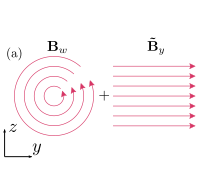
\includegraphics[width=0.8\textwidth]{figs/theory/wires/simplefield.pdf}
    \hfill{}
  \end{subfigure}
  \begin{subfigure}[b]{0.45\textwidth}
    \centering
    \import{figs/theory/wires/}{simpleheat_alone.pgf}
  \end{subfigure} \\
  \begin{subfigure}[b]{0.45\textwidth}
    \centering
    \import{figs/theory/wires/}{simpleheat_y.pgf}
  \end{subfigure}
  \begin{subfigure}[b]{0.45\textwidth}
    \centering
    \import{figs/theory/wires/}{simpleheat_z.pgf}
  \end{subfigure}
  \caption{
    The field from a simple two-dimensional wire trap. In subfigure (a) a wire carries
    current $I=\SI{1}{\milli\ampere}$ in the positive $x$ direction (out of the
    page) to create the usual field $\mathbf{B}_w$. This is combined with the
    external bias field $\mathbf{\tilde{B}}_y$ to create the two-dimensional trap
    at height $h=\SI{1}{\milli\meter}$
    shown in subfigure (b). The field lines are shown by pink arrows, and the
    magnitude of the resulting field is shown with the blue gradient (darker
    means weaker field, guide to the eye). Cut throughs of the potential are
    shown for $y$ (with $x=0$, $z=h$) in (c) and for $z$ (with $x = y = 0$) in
    (d).
  }
  \label{theory:fig:simplefield}
\end{figure}

Since the field minimum here is a zero, we can approximate the value near the
centre by a (two-dimensional) quadrupole with gradient
%
\begin{equation}
  B' = -\frac{2\pi \tilde{B}_y^2}{\mu_0 I}.
\end{equation}
%
The depth of the trap is $\mu \tilde{B}_y$, where $\mu$ is the magnetic dipole
moment of the trapped particle. This can be seen in
\mysubfigref{theory:fig:simplefield}{d}: the potential is $B = |B_w(z) +
\tilde{B}_y|$, and so has an asymptote at $B=|\tilde{B}_y|$ as
$z\rightarrow\infty$. We usually write this depth as a temperature
%
\begin{equation}
  T  = \frac{\mu \tilde{B}_y}{k_B}.
  \label{theory:eqn:depth}
\end{equation}
%
We can transform such a trap into a Ioffe-Pritchard trap by applying a second
bias field along the $x$ direction to lift the field minimum away from
zero.

Of course, it is commonly desirable to trap in all three dimensions. A simple
way to introduce confinement along the $x$ axis is to introduce a second wire
trap acting in the perpendicular direction. Such a device is called a dimple
trap (or cross conductor trap, or X-trap) and is illustrated in
\myfigref{theory:fig:dimple}. We label the current in the second wire $I_1$
and the new bias field, which is parallel to the $x$-axis and opposes the
$I_1$ field is labelled $\mathbf{B}_x$. In the case that $I_1 \ll I$, the
second wire can be treated as a perturbation of the first. The field minimum is
therefore still at $h$, and its depth is given by \myeqref{theory:eqn:depth}.

\begin{figure}[htb]
    \centering
    \begin{tabular}[t]{cc}
\begin{subfigure}{0.3\textwidth}
    \centering
    \smallskip
    \includegraphics[width=\textwidth]{figs/theory/wires/dimple.pdf}
\end{subfigure}
    &
        \begin{tabular}{c}% if you add [t], than sub images are pushed down
        \smallskip
            \begin{subfigure}[t]{0.4\textwidth}
                \centering
                  \import{figs/theory/wires/}{dimpleheat_alone.pgf}
            \end{subfigure}\\
            \begin{subfigure}[t]{0.4\textwidth}
                \centering
                  \import{figs/theory/wires/}{dimple_x.pgf}
            \end{subfigure}
        \end{tabular}\\
    \end{tabular}
  \caption{
    The geometry of the dimple trap is shown in subfigure (a), with the new
    wire along $y$ carrying current $I_1$ intersecting the $I$ wire. An
    additional bias field in the $x$ direction, $\tilde{B}_x$ creates the field
    minimum. The field lines (pink) and magnitude (blue, darker is weaker,
    guide to the eye) is shown in subfigure (b) along $x=0$. Note the strong
    field region along the $y$ axis around the $I_1$ wire. Subfigure (c) shows
    a cut through of the trapping potential in the $x$ direction with $y=0$,
    $z=h$.
  }
  \label{theory:fig:dimple}
\end{figure}

The dimple trap can be used as a quadrupole trap when the bias fields are
chosen to exactly cancel the magnetic field at the centre, or it can be used as
a Ioffe-Pritchard trap when there is a non-zero minimum. We will focus on the
latter case, in which case it is useful to write down the trap frequencies, the
derivation of which is similar to the one for the six-wire field discussed in
section~\ref{theory:magtraps}.
%
Since the trapping from the $I$ wire will be stronger than the $x$-axis
confinement from the $I_1 << I$ wire, we $\omega_x$ to be the weak trapping
direction. We again write down the field minimum
%
\begin{equation}
  B_0 = \left|\tilde{B}_x + \frac{\mu_0 I_1}{2\pi h}\right|,
\end{equation}
%
the transverse gradient
%
\begin{equation}
  B'_\perp = \frac{\mu_0 I}{2 \pi h^2},
\end{equation}
%
and the curvature along the weak component
%
\begin{equation}
  B'' = \frac{\mu I_1}{\pi h^3}.
\end{equation}
%
The trap frequency in the strong direction is
%
\begin{equation}
  \omega_\perp = \sqrt{\frac{\mu B_\perp'^2}{m B_0}}
  \label{theory:eqn:perpfreq}
\end{equation}
%
where $m$ is the particle mass. In the weak direction (along $x$) the frequency
is
%
\begin{equation}
  \omega_x = \sqrt{\frac{\mu B''}{m}}.
  \label{theory:eqn:xfreq}
\end{equation}

\subsection{The H-trap}

Consider the dimple trap, but with $\tilde{B}_x$ set to zero. Now what was
previously a magnetic field minimum will be a field maximum. By putting two
such dimple traps next to each other, it is possible to create a local minimum
within which we can trap molecules. Such a trap is called an H-trap, and is
pictured in \myfigref{theory:fig:Htrap}. We label the current due to the second
dimple trap $I_2$, and again note that the bias field in the $x$ direction can
be set to zero. The distance between $I_1$ and $I_2$ is denoted $d$, and we now
refer to the wire carrying current $I$ as the axis of the trap.

\begin{figure}[htb]
  \centering
  \begin{subfigure}[b]{0.4\textwidth}
    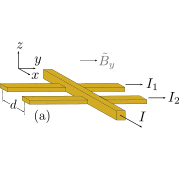
\includegraphics[width=\textwidth]{figs/theory/wires/Htrap.pdf}
    %\vspace{0.1mm}
  \end{subfigure}
  \begin{subfigure}[b]{0.4\textwidth}
    \import{figs/theory/wires/}{Hx.pgf}
  \end{subfigure}
  \caption{The geometry of the H-trap is shown in subfigure (a). In subfigure
  (b) we show the potential for an H-trap with
  $I_1=I_2=I/10=\SI{0.1}{\milli\ampere}$ and $d=\SI{10}{\milli\meter}$. Again the bias field is chosen so
  that $h=\SI{1}{\milli\meter}$.}
  \label{theory:fig:Htrap}
\end{figure}

We note that we need not choose $I_1$ and $I_2$ to be the same, although from
now on we will assume that they have the same magnitude, the sign can differ.
In other words these currents can be parallel or anti-parallel. In the former
case the trap forms a Ioffe-Pritchard trap; this is due to the fields from
$I_1$ and $I_2$ adding in the centre, to provide some overall non-zero
component in the $x$ direction. When the currents are anti-paraellel, the $I_1$
field opposes the $I_2$ field in the centre of the trap, the two cancel and
there is a field zero. Hence the latter configuration is a quadrupole trap.

In the Ioffe-Pritchard configuration, we can write down the field's
minimum
%
\begin{equation}
  B_0 = \tilde{B}_x + 2\tilde{B}_y \frac{I_1}{I}\frac{h^2}{(d/2)^2 + h^2}
\end{equation}
%
transverse gradient
%
\begin{equation}
  B'_\perp = \frac{2\pi\tilde{B}_y}{\mu_0 I}
\end{equation}
%
and curvature~\cite{PhysRevA.79.013407}
%
\begin{equation}
  B'' = \tilde{B}_x + 2\tilde{B}_y\frac{I_1}{I_0}\frac{h^2}{(d/2)^2+h^2}
\end{equation}
%
and the trap frequencies are again given by equations~\ref{theory:eqn:perpfreq}
and~\ref{theory:eqn:xfreq}~\cite{PhysRevA.79.013407}. In the quadrupole
configuration, the traps is characterised by the perpendicular gradient
$B'_\perp$. 

\subsection{Three dimensional single-wire traps}

Although the H-trap provides a method of creating a three dimensional
microtrap, it is not always convenient to have to use three distinct wires.
Fortunately the H-trap can be approximated by a single wire, either in a
U-shape for the quadrupole variant, or a Z-shape for the Ioffe-Pritchard
variant. These are pictured in \myfigref{theory:fig:HUZ}. Note that for the U-trap
the currents in the off-axis wires are once again anti-parallel, and in the
Z-trap these currents are parallel. For the U- and Z-traps, we denote the
distance between the end wires as $d$, and again refer to this as the axis.

\begin{figure}[htbp]
  \centering
  
\includegraphics[width=\textwidth]{figs/theory/wires/HUZcomp.pdf}
  \caption{Current configuration for U-trap (Z-trap) approximating the
  quadrupole (Ioffe-Pritchard) H-trap configuration.}
  \label{theory:fig:HUZ}
\end{figure}

The Z-trap will be the primary focus of this thesis, and so we will focus on
this as an example. In \myfigref{theory:fig:HZcontours} we compare an H-trap
with a current of \SI{1}{\milli\ampere} on each wire with the potential due to
a single Z-wire also with current \SI{1}{\milli\ampere}. In both cases
$d=\SI{10}{\milli\meter}$, and a bias field of \SI{2}{\milli\gauss} in the $y$
direction is chosen, so as to create a minimum at approximately
$z=\SI{1}{\milli\meter}$ from the axis. The potentials are similarily
comparable for the H-trap in quadrupole configuration and the U-trap.

\begin{figure}[htbp]
  \centering
  \import{figs/theory/wires/}{HZcontours.pgf}
  \caption{Contour plots comparing the potentials for a H-trap in
    Ioffe-Pritchard configuration (left column) and Z-trap (right column), with
    cut throughs for $z=\SI{1}{\milli\meter}$ (top row) and $x=0$ (bottom row).
    All wires carry a current of $I=\SI{1}{\milli\ampere}$ and a bias field of
    \SI{2}{\milli\gauss} is applied in the $y$ direction.}
  \label{theory:fig:HZcontours}
\end{figure}

This illustrates that a single current-carrying wire can be used to form a trap
in three dimensions. The examples here use length scales of a few millimeters,
and have typical depths of \SI{100}{\nano\kelvin}, but we will discuss in
chapter~\ref{sim} that it is possible to realise much smaller trap and deeper
traps.


\section{Physics of diatomic molecules}
\label{theory:molecules}

Up to this point we have considered abstracted and idealised systems, but in
the next chapter we will begin to think about the realities of implementing a
cold molecule experiment. It is essential that we introduce and understand the
energy structure of diatomic molecules, which is far richer and more complex
than the structure of atoms, due to the additional effects of vibration and
rotation of the two nuclei. This section will explain the physics of diatomic
molecules so that the particulars of the cooling transitions and magnetically
trappable states can be easily explained in the next chapter. A far more
detailed review of the topic can be found in \inlineref{brown_carrington_2003}.

\subsection{Electronic, vibrational, and rotational energy}

We can begin by considering two atoms or ions, which we label $A$ and $B$,
with masses  $m_i = m_p Z_i$, $i\in\{A,B\}$ and $m_p$ is the proton rest mass. We say that the location of the
atoms is $\mathbf{R}_i$ and the distance between them is
$R_{AB}$ where $\mathbf{R}_{AB} = \mathbf{R}_B - \mathbf{R}_A$. In the case
that $R_{AB} \rightarrow \infty$ we have two distinct atoms that will behave 
as we would expect them to in isolation (see, for example,
\inlineref{Foot2005}).

As $R_{AB}$ is reduced, the atoms will begin to perturb each other, with the
perturbation dominated by the Coloumb interaction between the various charges.
We can write down the Hamiltonian of such a system, and it is most useful to do
so in the centre of mass (COM) frame, with the reduced mass
%
\begin{equation}
  \mred{} = \frac{m_A m_B}{m_A + m_B}
\end{equation}
%
and COM location
%
\begin{equation}
  \mathbf{R}_\text{COM} = \frac{m_A \mathbf{R}_a + m_B \mathbf{R}_b}{m_A+m_B}.
\end{equation}
%
The Hamiltonian is then the sum of the terms arising from the Coulomb
interaction, and the motion of the molecules
%
\begin{equation}
  H = T_n + T_e + V_{nn} + V_{en} + V_{ee}
\end{equation}
%
where
%
\begin{align}
  T_n &= -\frac{\hbar^2}{2\mred{}}\nabla_{AB}^2\\
  T_e &= -\frac{\hbar^2}{2 m_e}\sum_{i=1}^{N_e} \nabla_i'^2 -
  \frac{\hbar^2}{2(m_A + m_B)}\sum_{i, j} \nabla'_i \cdot \nabla'_j \\
  V_{nn} &= \frac{Z_A Z_b e^2}{4\pi\epsilon_0 R_{AB}} \\
  V_{en} &= - \frac{e^2}{4\pi\epsilon_0}\sum_{i=1}^N \left(\frac{Z_A}{R_{Ai}} + \frac{Z_B}{R_{Bi}}\right) \\
  V_{ee} &= \frac{e^2}{4\pi\epsilon_0}\sum_{i<j} \frac{1}{R_{ij}}
\end{align}
%
and we have introduced the relative distances $R_{ij}$ being the distance
between the $i^\text{th}$ and $j^\text{th}$ electrons, and $R_{Ai}$ the
distance between $A$ and the $i^\text{th}$ electron (and similar for $B$) as
shown in \myfigref{theory:fig:mol}. The total number of electrons is
$N_e$. The primed gradient operators represent differentiation with respect to
the COM coordinates.
%
The time-independent Schr\"odinger equation (TISE),
%
\begin{equation}
  H\psi = E\psi
\end{equation}
%
can now be solved for this Hamiltonian, although we will only sketch the
solution here. A full derivation can be found in \inlineref{brown_carrington_2003}.

\begin{figure}
  \centering
  \includegraphics[width=0.25\textwidth]{figs/theory/mols.pdf}
  \caption{
    The geometery of a diatomic molecule, with relevant vectors labelled.
    Nucleii in blue and pink, electrons in purple.
  }
  \label{theory:fig:mol}
\end{figure}


\subsubsection{Electronic states}

The wavefunction
$\psi$ is a function of $\mathbf{R}_{AB}$ and the position of each of the
electrons, that is
%
\begin{equation}
  \psi = \psi(\mathbf{R}_{AB}, \mathbf{R}_1, \dots \mathbf{R}_{N_e}).
\end{equation}
%
We now make the Born-Oppenheimer approximation, where we say that due to the
fact that the nuclear mass is much higher than that of the electrons, the
nucleii are stationary on the timescale of the electronic motion. For this
reason we are able to separate the wavefunction into the electronic and nuclear
parts
%
\begin{equation}
  \psi(\mathbf{R}_{AB}, \mathbf{r}) = \psi_e(\mathbf{R}_{AB}; \mathbf{r})
  \psi_n(\mathbf{R}_{AB}).
\end{equation}
%
Note here that $\mathbf{R}_{AB}$ is treated as a parameter of $\psi_e$ and we
have introduced $\mathbf{r} = \{\mathbf{R}_1, \dots \mathbf{R}_{N_e} \}$ to
represent the set of electronic coordinates.

There is then a separate electronic TISE
%
\begin{equation}
  H_e \psi_e(\mathbf{R}_{AB}; \mathbf{r}) = E_e(R_{AB}, \mathbf{r})\psi_e(\mathbf{R}_{AB};
  \mathbf{r})
  \label{theory:eqn:TISEelectron}
\end{equation}
%
where the Hamiltonian $H_e = H - T_n$ is the previous Hamiltonian but excluding
the term for the nuclear motion, because these are stationary in the
Born-Oppenheimer approximation. This problem now begins to resemble the
analogous one of finding the electronic states of atoms, and can be solved by
similar numerical methods~\cite{Foot2005}. The upshot is that it is possible to
determine the electron eigenstates, which we label $\psi_e(\mathbf{R}_{AB};
q)$, with $q$ being the quantum number for the electronic
configuration\footnote{The numbering of the electronic configurations is
actually more complicated than this. We will discuss how these states are
labelled in section~\ref{theory:qnos}.}. The
energy of the state is now denoted $E_e(q; R_{AB})$, with $q$ as a parameter
and $E_e$ a function of  $R_{AB}$.
It is common to approximate this energy as the Morse potential
%
\begin{equation}
  E_e(q; R_{AB}) = D(1-e^{-\beta(R_{AB} - R_{AB}^0)})^2
\end{equation}
%
where $R_{AB}^0$ is the equilibrium displacement of the nucleii, $D$ is the
dissociation energy, and $\beta$ is a parameter for the width of the
potential. All of these are dependent on the electronic configuration, but this
dependence is suppressed in the notation. On a long timescale, the $E_e$
dependence on $R_{AB}$ averages away, and so $E_e = E_e(q)$.

Implicit in the Born-Oppenheimer approximation is that the electronic
configuration is the largest contribution to the state's energy. We can make a
na\"ive estimate of this energy as the typical kinetic energy of the electrons
%
\begin{equation}
  E_e \approx \frac{p^2}{2m_e} = \frac{\hbar^2}{2m_e a^2}
\end{equation}
%
where $a\sim\SI{1}{\angstrom}$ is the lengthscale of the molecule and $m_e$ is
the electron mass, so that $E_e/h \sim \SI{1000}{\tera\hertz}$. This
gives us the first order contribution to the energy of the molecule. 

\subsubsection{Nuclear motion}

We now turn our attention to the nuclear wavefunction. With a bit of
work~\cite{brown_carrington_2003} it is possible to write down the relevant
TISE
%
\begin{equation}
  \left(-\frac{\hbar^2}{2\mred{}}\nabla_{AB}^2 + E_e(q; R_{AB}) -
  E\right)\psi_n(\mathbf{R}_{AB}) = 0.
  \label{theory:eqn:nucTISE}
\end{equation}
%
Note that the potential that the nucleii move through is the potential
generated by the electron configuration, and that this potential is central. We
can therefore anticipate the separation of the nuclear wavefunction into radial
and angular parts,
%
\begin{equation}
  \psi_n(\mathbf{R}_{AB}) = \frac{1}{R_{AB}}f(R_{AB})Y_{R, m_R}(\theta, \phi),
  \label{theory:eqn:nucsep}
\end{equation}
%
where we choose the factor of $1/R_{AB}$ to simplify the equation in the rest
of the section. We will introduce the operator $\mathbf{R}$ to describe the
rotational angular momentum. The angular part of the solution is given by the usual
spherical harmonics $Y_{R, m_R}$ where
%
\begin{align}
  \mathbf{R}^2 Y_{R, m_R} &= R(R+1) Y_{R, m_R} \\
  R_z Y_{R, m_R} &= m_R Y_{R, m_R}
\end{align}

the rotational quantum number for
the state, and $M_N$ is the projection onto the nuclear axis.

Substitution of \myeqref{theory:eqn:nucsep} into \myeqref{theory:eqn:nucTISE}
yields 
%
\begin{equation}
  \left(-\frac{\hbar^2}{2\mred{}}\frac{\dd^2}{\dd R_{AB}^2} +
    \frac{\hbar^2 R(R+1)}{2\mred{}R_{AB}^2} + E_e(q; R_{AB}) - E\right)f(R_{AB}).
\end{equation}
%
where we have expanded $\nabla_{AB}^2$ in terms of the second derivative in
$R_{AB}$ and the angular momentum operator $\mathbf{N}^2$. This equation is now
that of an oscillator in the Morse potential $E_e(q; R_{AB})$, with an
additional energy term that arises due to the rotation,
%
\begin{equation} E_\text{rot}(R) = \frac{R(R+1)}{2\mred{} R_{AB}^2}.
\label{theory:eqn:rotenergy} \end{equation}

The vibrational part of the wavefunction can be solved by the standard
computational methods for finding the wavefunctions of anharmonic
potentials~\cite{Foot2005}. These vibrational states form the usual ladder of
% TODO Check this Binney cite OK? Does he really do this?
states inside an anharmonic potential~\cite{Binney} as pictured in
\myfigref{theory:fig:vibtrans}. We label these states with the quantum number
$v$, and so re-write $f(R_{AB}) = f_v(R_{AB})$ to clarify which vibrational
level we are referring to.

At low energy the Morse potential approximates
to a harmonic potential
%
\begin{equation}
  E_e(q; R_{AB}) \approx D\beta^2(R_{AB} - R_{AB}^0)^2
\end{equation}
%
where the vibrational frequency is related to the potential by
%
\begin{equation}
  \frac{1}{2}\mred{}\omega_\text{vib}^2(R_{AB}-R_{AB}^0)^2 = D\beta^2(R_{AB}-R_{AB}^0)^2.
  \label{theory:eqn:vibfreqrel}
\end{equation}  
%
We can estimate this vibrational frequency by considering the opposite limit,
near dissociation. We approximate $D$ to be the typical electronic energy $E_e$
and note that for dissociation to occur we expect $\beta(R_{AB} - R_{AB}^0) >
1$ and also that at this point $(R_{AB} - R_{AB}^0)^2\sim a^2$. We therefore
substitute into \myeqref{theory:eqn:vibfreqrel} $D\approx E_e$ and
$\beta\approx a^{-1}$
%
\begin{equation}
  \hbar\omega_\text{vib} \approx \sqrt{\frac{\hbar^4}{\mred{} m_e a^4}} \sim
    h\times\SI{10}{\tera\hertz}.
\end{equation}
%
where we took $\mred{}\approx m_e$.

We now have and estimate for the vibrational energy, and the final step is to
compare this to the rotational energy in \myeqref{theory:eqn:rotenergy}, where
we expect typical values
%
\begin{equation}
  E_\text{rot} = \frac{\hbar}{2 \mred{} R^0_{AB}} \sim h\times\SI{100}{\giga\hertz}
\end{equation}
%
it is clear that the vibrational energy levels further perturb the vibrational
levels.

\subsubsection{Qualitative summary}

We have described how the wavefunction of a diatomic molecule in free space can
be written as three separate wavefunctions, one each for the electronic,
vibrational and rotational Hamiltonians. We denote the wavefunction in terms of
the good quantum numbers
%
\begin{equation}
  \psi(q, v, R, M_R) = \frac{1}{R_{AB}}\psi_e(\mathbf{R}_{AB};q)
  f_v(R_{AB})Y_{N, M_N}(\theta, \phi).
\end{equation}
%
The Born-Oppenheimer approximation states that the electrons move on a much
faster timescale than the nucleii, and hence have a higher energy (by about a
factor of $100$) than the nuclear motional energy.

Due to this difference in timescale, the nucleii move in the electrostatic potential
generated by the nucleii, which can be approximated to be a Morse potential. This
means that the nucleii vibrate as an anharmonic oscillator, with some
equilibrium distance $R_{AB}^0$. The vibrational motion is again higher (by
about a factor of $100$) than the rotational energy, which comes from the
tumbling of the two nucleii. The total energy is
%
\begin{equation}
  E(q,v,R) = E_e(q) + E_\text{vib}(v) + E_\text{rot}(R).
\end{equation}


\subsection{Transitions}

% Just basic ideas or electronic, vibrational, ro-vibrational transitions.
% Talk more about microwave spectroscopy elsewhere?

We will now state without derivation, the selection rules describing the
allowed transitions between the various states of the molecule. We will label the original state in
the transition $\ket{1} = \ket{q, v, R, m_R}$ and the final state $\ket{2} =
\ket{q', v', R', m_R'}$.
%
It is useful to remember that the following results are found by considering
the intensity of the transition, which is proportional to $|d_{12}|^2$, where
%
\begin{equation}
  d_{12} = \bra{1}\mathbf{d}\cdot\mathbf{\epsilon}\ket{2}
\end{equation}
%
is the matrix element of the transition, $\mathbf{d}$ is the dipole matrix
operator, and $\mathbf{\epsilon}$ is a vector representing the polarisation of
the light.

This matrix element is evaluated by re-writing in a spherical basis, then
writing this basis so that the $z$ axis is aligned with the internuclear axis.
This yields an integral over the electronic, vibrational and rotational
wavefunctions. Deriving this integral and its solution is beyond the scope of
this discussion, as it is not required to understand the rest of the thesis. It
has been explained eloquently and succinctly in various texts, including
\inlineref{brown_carrington_2003}.

\subsubsection{Pure rotational transitions}

In a pure rotational transition $q'=q$ and $v'=v$. Such transitions are
permitted only when $\Delta R = R' - R = \pm1$. The selection rule for $M_R$ is
dependent on the polarisation of the transition light. For linearly polarised
light $\Delta M_R = M_R' - M_R =
0$, whereas for circularly polarised light $\Delta M_R =  \pm1$ for
$\sigma^\mp$ polarised light.

\subsubsection{Vibrational transitions}

In the case where $q'=q$ we have the same selection rules for any change in the
rotational quantum numbers. It can be shown that the additional selection rule
for the vibrational transition is $\Delta v = v' - v = \pm 1$. Of course,
$\Delta v = 0$ is allowed, but then this reduces to the above case of a pure
rotational transition.

\subsubsection{Changing the electronic state}

When the electronic state changes the analysis is more complicated, and there
are no consistent selection rules. This can be explained when we recall that
the matrix element $d_{12}$ is an integral over the state's wavefunction $\psi
= R_{AB}^{-1}\psi_ef_v(R_{AB}) Y_{R, M_R}$. When the
electronic states are the same, the electronic contribution becomes a factor of
one and the vibrational states are all states from the same anharmonic
oscillator, as can be seen in \myfigref{theory:fig:vibtrans}. In this case we
can derive the above selection rules.

\begin{figure}
  \centering
  \includegraphics[height=0.4\textwidth]{figs/theory/vibtrans.pdf}
  \caption{
    A cartoon depiction of a transition between electronic states. Various
    vibrational wavefunctions (blue) are shown for two electronic potentials.
    The $0\rightarrow0$ transition is weak, since there is small overlap
    between the vibrational wavefunctions, but the $0\rightarrow4$ transition
    (dashed line) is stronger.
  }
  \label{theory:fig:vibtrans}
\end{figure}

Now that $q\neq q'$, the vibrational states are not states of the same
anharmonic potential, and so the overlap integral of the wave functions must
be computed numerically. The vibrational component of this integral is called
the Franck-Condon factor, and is written as
%
\begin{equation}
  q_{v',v} = \left|\int f*_v(R_{AB}f_v(R_{AB})\dd R_{AB}\right|^2.
\end{equation}
%
The rotational state can change by the same selection rules as before, except
in the case that the rotational angular momentum is coupled to the angular
momentum of the electrons. In this case we can have $J$ as the good quantum
number, with a selection rule $\Delta J = 0, \pm1$.


\subsection{Good quantum numbers}
\label{theory:qnos}

We will now briefly review the quantum numbers that we have introduced to
describe the molecule state. First note that the quantum number for the
electronic level is not really a quantum number at all. It obfuscates the true
quantum numbers, which come from the angular momentum operators for the
electrons. We will describe the good quantum numbers for two of Hund's
cases~\cite{brown_carrington_2003}, which differ depending on how strongly each
of the angular momentum operators couple to each other. They are pictured in
\myfigref{theory:fig:hund}.

\begin{figure}
  \centering
  \includegraphics[width=0.8\textwidth]{figs/theory/hund2.pdf}
  \caption{Coupling schemes in Hund's (a) and (b) cases. In (a) the
    $\mathbf{L}$ (gold) and $\mathbf{S}$ (purple) precession about the axis is
    shown by the dashed circles. The black circle represents the precession of
    $\mathbf{\Omega} (\approx\mathbf{L}+\mathbf{S})$ and $\mathbf{R}$ around
    $\mathbf{J}$. In (b) $\mathbf{L}$ (gold) precesses rapidly around the axis
    as shown by the dashed circle. $\mathbf{R}$ couples to
    $\Lambda\mathbf{\mathbf{\hat{e}}}(\approx\mathbf{L})$, and these precess
    around $\mathbf{N}$ (purple circle). $\mathbf{N}$ and $\mathbf{S}$ precess
    around $\mathbf{J}$ (black circle). The good quantum numbers are summarised
    in the bottom row. This figure is adapted from
    \inlineref{brown_carrington_2003}.
  }
  \label{theory:fig:hund}
\end{figure}


In the first case (a), the electron orbital angular momentum $\mathbf{L}$ is
strongly coupled to the molecular axis, and the spin angular momentum
$\mathbf{S}$ couples strongly to $\mathbf{L}$. Hence, these momenta both
precess around the molecular axis. The good quantum numbers associated with
these operators are their projections onto the axis which we label $\Lambda$
and $\Sigma$  respectively, as well as $S$. $L$ is not a good quantum number
since it couples very stongly to the axis and so precesses rapidly around it.

The rotation operator $\mathbf{R}$ coupling is even weaker, and hence can be
approximated to couple to the projection of $\mathbf{L} + \mathbf{S}$ onto the
axis. We label this projection $\mathbf{\Omega} = \Omega \mathbf{\hat{e}}$
where $\mathbf{\hat{e}}$ is the unit vector along the axis, and $\Omega =
\Lambda + \Sigma$. The total angular momentum is $\mathbf{J} = \mathbf{L} +
\mathbf{S} + \mathbf{N}$. Again, due to the rapid precession of $\mathbf{L}$
and $\mathbf{S}$, we show this in the figure as a precession of
$\mathbf{\Omega}$ and $\mathbf{R}$ around $\mathbf{J}$. Note that
$\mathbf{\Omega}$ is not truly an operator, and is only useful for illustrative
purposes.

In the second case of interest (b), $\mathbf{L}$ is strongly coupled to the
axis as before, and its projection onto the axis again creates a good quantum
number $\Lambda$. $L$ is not a good number for the same reason as before.
$\mathbf{R}$ has the next strongest coupling, so we define a new operator
$\mathbf{N} = \mathbf{L} + \mathbf{R}$, which for illustrative purposes we show
in the figure as $\Lambda \mathbf{\hat{e}} + \mathbf{R}$.  $\mathbf{N}$ and
$\mathbf{S}$ now couple and precess around $\mathbf{J} = \mathbf{N} +
\mathbf{S}$. The good quantum numbers for both cases are summarised in the
figure. If $L=0$ for a state then it will obey this case.

We label these states by spectroscopic notation taking the form
%
\begin{equation*} 
  X^{2S+1}|\Lambda|^\pm_{|\Omega|}
\end{equation*}
%
where $X$ is used to represent the ground state, but for higher states this is
replaced by incrementing letters of the alphabet, starting with $A$ for the
first excited state. $\Lambda$ is not represented by its numerical value, but
by the Greek characters $\Sigma$, $\Pi$, $\Delta$, etc.\ in analogy with the
notation for the orhital states in atoms. The superscript $\pm$ represents the
parity of the wavefunction on reflection. When $\Omega$ is redundant it can be
omitted.

Up to this point we have mainly denoted the wavefunctions as functions, but we
will soon find it useful to write the states using braket notation. We will not
denote electronic states, this way, but will describe the other quantum
numbers. For example, we may write for a Hund (b) case state $\ket{N, S, J,
\Lambda}$. However, for an electronic state where $L=0$, we could express this
in an equivalent manner such as $\ket{N, m_N}_\text{rot}\ket{S, m_S}$. The
quantum number that the ket refers to is implicit by its contents.
%
%TODO In this case remove ket{*}_rot subscripts, OR ammend this sentence, eg:
% "or is specified to be a rotational state by the subscript
% $\ket{*}_\text{rot}$"

\subsection{Hyperfine structure}

These states can be further split into hyperfine states by the angular momentum
contribution of the nuclear spin, which has operator $\mathbf{I}$. The new
total angular momentum is  $\mathbf{F} = \mathbf{J} + \mathbf{I}$. These states
will be important later, since the $m_F$ substates will be used as weak-field
seekers for magnetic trapping.

% TODO MOVE THIS
\subsection{Cavity quantum electrodynamics}

\cm{This section is getting moved to microwaves. Need to ensure that when
moved, any motivation pointing in this direction also moves.}

% TODO Can probably get rid of a lot of this, depends on context of where I put
% it.
A key part of the motivation for a molecule chip trap is the idea that
integrated microwave guides can be used to couple photons to the rotational
transitions of the molecules. Of particular interest is the idea
that a resonator can be used to perform this coupling, leading to the
ability to perform sideband-cooling to the motional ground state, state readout
and coupling between individually-trapped molecules~\cite{Andre2006}. This is
similar to techniques used in atom chips~\cite{Treutlein2008} and for optical
resonators coupling to atomic energy levels~\cite{SchleierSmith2011}.
% TODO Better cite in this last bit?

For our purposes, the coupling of a single molecule and the microwave field can
be treated as the coupling of a two-level system to a quantum mode of a cavity
field. The canonical description of such a system is given by the familiar
Jaynes-Cummings Hamiltonian (JCH) in the rotating wave
approximation~\cite{gerry_knight_2004}
%
\begin{equation}
  H_\text{JC} = \hbar\omega_c a^\dagger a + \frac{\hbar \omega_0}{2} \sigma_z +
  \frac{\hbar\Omega}{2}(a^\dagger \sigma_- + a\sigma_+)
  \label{theory:eqn:JCH}
\end{equation}
%
where $a$ ($a^\dagger$) is the annihilation (creation) operator of the photons,
$\Omega$ is the Rabi frequency of the interaction, $\sigma_i$ with $i\in{x, y,
z}$ are the Pauli matrices, and $\sigma_\pm =
(\sigma_x \pm i\sigma_y)/2$ are the raising and lowering operators of the
molecule state. The
detuning of the cavity resonance from that of the spin is $\Delta = \omega_0 -
\omega_c$. The system is shown in \mysubfigref{theory:fig:JCHstates}{a}.

\begin{figure}
  %\includegraphics{}
  \cm{Part (a) is image of JCH system, (b) is state manifold without coupling
  or detuning, (c) is state manifold with coupling (d) adds detuning (similar
  to Bohi fig 1)}
  \caption{\cm{TODO}}
  \label{theory:fig:JCHstates}
\end{figure}

We denote the ground (exicted) state of the molecule as $\ket{g}$ ($\ket{e}$).
The light field state can be taken to be a Fock state ($\ket{n}$ with $n \in
\mathbb{Z}$). Note that the final term in equation~\ref{theory:eqn:JCH}) has
the effect of exciting the ground state while absorbing a photon
($\ket{g}\ket{n} \leftrightarrow \ket{e}\ket{n-1}$) or lowering the excited state
and releasing a photon ($\ket{e}\ket{n} \leftrightarrow \ket{g}\ket{n+1}$).

Following the procedure in \inlineref{gerry_knight_2004}, we can see that this
mixing of the states results in a shift of the energy levels to create the
dressed states
%
\begin{align}
  \ket{+, n} &= \cos\Phi_n \ket{g}\ket{n} + \sin\Phi_n \ket{e}\ket{n+1} \\
  \ket{-, n} &= -\sin\Phi_n \ket{g}\ket{n} + \cos\Phi_n \ket{e}\ket{n+1}
\end{align}
%
with
%
\begin{equation}
  \tan(2\Phi_n) = \frac{\Omega\sqrt{n+1}}{\Delta}
\end{equation}
%
and having shifted energies
%
\begin{equation}
  E_{\pm, n} = (n+1)\hbar\omega_c \pm \frac{\hbar}{2}\sqrt{\Omega^2(n+1) +
  \Delta^2}.
  \label{theory:eqn:JCHenergies}
\end{equation}
%
It is useful to consider the manifold of states as depicted in
\myfigref{theory:fig:JCHstates}.  
%TODO This fig
Note that in the limit of no coupling
($\Omega = 0$) and no detuning ($\Delta = 0$) the energies are that of the bare
states, and $\ket{g}\ket{n+1}$ is degenerate with $\ket{e}\ket{n}$, as in part
(b) of the subfigure. Introducing coupling ($\Omega \neq 0$) lifts this
degeneracy, as in part (c). When the detuning is non-zero ($\Delta \neq 0$)
there is additional offset due to the second term in
\myeqref{theory:eqn:JCHenergies}, see part (d) of the figure.

The strong coupling r\'egime is reached when the coupling $g=2\Omega$ is
greater than the rate of decay from the cavity $\kappa = \omega_0 / Q$, where
$Q$ is called the quality factor of the cavity. The coupling parameter is
related to the transition dipole moment $d$ and the amplitude of the electric
field $E_0$ by
%
\begin{equation}
  \hbar g = \frac{d E_0}{2}.
\end{equation}
%
For the resonator, the amplitude of the electric field can be expressed in
terms of the cavity parameters by considering the electric field density
%
\begin{equation}
  \frac{1}{2} \epsilon_0 E_0 = \frac{\hbar \omega_0}{V}
\end{equation}
%
where $V$ is the volume of the mode in the cavity. The idea is to confine the
molecules in a trap that is on the $w=\SI{10}{\micro\meter}$ scale (see
chapter~\ref{overview}) and the resonator will necessarily have a length on the
scale of $\lambda_0 = 2\pi c / \omega_0$, therefore $V\approx w^2\lambda_0$.
Hence we have that
%
\begin{equation}
  g = \sqrt{\frac{2\pi c d^2}{\hbar \epsilon_0 w^2 \lambda_0^2}}.
\end{equation}

% TODO maybe move this whole sentence above
For the rotational \CaF{} transitions that we introduced above, in
section~\ref{theory:molecules} $d = \mu/\sqrt{3}$ with $\mu =
\SI{31}{\debye}$.
%
The coupling strength is therefore expected to be
%
% See nbs/2022-02-08_coupling.nb
\begin{equation}
  \frac{g}{2\pi} = \SI{20}{\kilo\hertz}
\end{equation}
%
and for strong coupling a cavity quality of
%
\begin{equation}
  Q = \frac{\omega_0}{g} > 1.7 \times 10^5
\end{equation}
%
is required.


\chapter{Overview of the experiment}
\label{overview}
%This chapter describes the process of desigining the molecule chip experiment.
This was motivated by three main factors: the need to integrate with the
existing experiment, the core proposal of confining molecules close to a
microwave guide, and the practicalities of fabricating the chip. Here I will
focus on how the first two factors informed the design choices, with changes
due to fabrication discussed in chapter~\ref{fab}. The design will be further
justified by simulation in chapter~\ref{sim}.

We begin with a discussion of
the existing experiment, and where the chip fits into it. I will then discuss
the process that lead us to choose a magnetic trap for our design. I will
present the final design \cm{and how it can be integrated with the existing
apparatus}. 

\section{Existing \CaF{} apparatus}

In this section I will present a summary of the process used to produce
ultracold \CaF{} molecules in a magnetic trap, which we intend to load onto the
chip trap. We will consider the various stages of the process, which is
presented in \myfigref{overview:fig:CaFcartoon}. First a beam of \CaF{}
molecules is created using a buffer gas
source~\cite{doi:10.1080/09500340.2017.1384516}. The beam is then slowed by
application of slowing light opposing its direction of
travel~\cite{Truppe2017a}. The slowing light can also be applied in the
transverse direction to reduce the broadening of the beam during its flight.
The molecules are captured in a MOT~\cite{Williams2017} and cooled in optical
molasses~\cite{Truppe2017} before being optically pumped into a weak field
seeking state~\cite{WilliamsMagnetic2018}. This allows for magnetic trapping
and transport of the molecules.

\begin{figure}
  \cm{TODO: Cartoon of CaF experiment up to MOT chamber}
  \caption{}
  \label{overview:fig:CaFcartoon}
\end{figure}

\subsection*{Buffer gas source}

In the buffer gas source, a copper cell containing a \cm{calcium} target is
cooled to \SI{4}{\kelvin}. \cm{Helium} (the eponymous buffer gas) flows into
the cell, thermalises with the cell walls and flows out through the exit
aperture. \cm{SF6} is also injected into the cell, and a high-power \cm{ndyag}
laser is fired at the target. The laser ablates the \cm{calcium} target,
producing \cm{Ca atoms} which react with the \cm{SF6} to produce \CaF{}
molecules which thermalise with the \cm{helium} and follow the flow out of the
exit aperture.  The result is a pulsed beam of \CaF{} molecules with typical
mean velocity \SI{160}{\meter\per\second}.

\subsection*{Slowing the beam}

The beam velocity can be further reduced by application of a counter-propagating
beam of slowing light. The light is resonant with the \cm{$X(v=0)\rightarrow
B$} transition \cm{($\mathcal{L^S_{00}}$}. A \SI{5}{\gauss} magnetic field is
applied, and the slowing light is linearly polarised at a relative
\SI{45}{\degree} angle, to remix dark ground states. The slowing light is
combined with repump light from \cm{$X(v=1)\rightarrow A(v=0)$, $\mathcal{L}_{10}$}
to avoid losing molecules that scatter into \cm{$X(v=1)$}. Since the molecules'
velocity will decrease during the slowing, the Doppler shift of the transition
frequency will also change. We account for this by chirping the slowing light,
and broadening the repump light. This process can reduce the molecule velocity
to \cm{??}.

\subsection*{Transverse cooling}

Slowing the beam has the undesirable effect of increasing the transverse
velocity of the molecules. This is due to the random walk of the molecules as
they scatter photons from the slowing light. To counteract this we apply
slowing beams in the transverse direction, also on the $\mathcal{L}_{00}^S$
transition. The slowing procedure described above is carried out
simultaneously, providing the remixing of dark ground states and the $v=1$
repump light.
%
Scattering of light in the transverse direction can collimate the beam, and has
been shown to improve the population of the MOT by a factor of $\sim3$. 

\subsection*{Capture in a MOT}

The \CaF{} beam travels \cm{some distance}, undergoing slowing and transverse
cooling before reaching the MOT chamber, where we capture the molecules. The
\CaF{} MOT is a type-II MOT~\cite{}, meaning that the angular momentum of the
excited state ($A(v=0)$, with $F'=1$) is greater than that of the ground state
($X(v=0)$ with $F=2$). Unlike a type-I MOT, it is therefore possible for a
molecule that has been pumped into the excited state to decay into a dark
state, or into a state that is anti-trapped by the MOT~\cite{}.

To resolve this, a dual-frequency MOT is employed. The main MOT transition is
addressed by the \pewpew{C}{00} light, with r.f.\ sidebands added to address
the different hyperfine levels. The sideband addressing the $F=1$ hyperfine
state is given opposite polarisation, and simultaneously serves as a second
frequency for the $F=2$ state, ensuring that the normally anti-trapped states
are repumped by the restoring beam into the MOT cycle. This is shown in \cm{a
figure}. The $F=2$ level is now strongly trapped and although the other levels
remain weakly trapped, this is sufficient to create a strong MOT.

The branching ratios of \CaF{} mean that the excited state can decay into
$X(v>0)$ states. One of the chief reasons that \CaF{} is chosen for our
experiment is that it has highly diagonal Franck-Condon factors, and so the
decay into these other states is minimised. However it is still essential to
repump the $X(v=1,2,3)$ states, which we do with the \pewpew{}{10}
\pewpew{}{21} and \pewpew{}{32} lasers respectively. Once again, r.f.\
sidebands are added to address the hyperfine levels of the $X$ state.

The capture velocity of the MOT is \cm{??} meaning that we are typically able
to capture $??$ molecules from our beam. The MOT population can be estimated by
looking at the scatter, or by turning off the light and performing
light-induced fluorescence imaging using \pewpew{C}{00}. The MOT temperature is
typically \cm{}, and this can be further reduced by lowering the intensity of
\pewpew{C}{00}~\cite{Truppe2017} \cm{what is final temp?}

\subsection*{Optical molasses}

Sub-Doppler cooling of \CaF{} is achievable by employing a blue-detuned
molasses. In this scheme the MOT coils are switched off, and \pewpew{C}{00}
is detuned to be blue-detuned \cm{by how much?}.  Consider the example of a
$F=1$ hyperfine level ground state, and $F=0$ excited state which is shown in
\cm{fig like Hannah's 5.1}. A polarisation gradient is established across the
molasses. In regions where the polarisation is $\sigma_-$ ($\sigma_-$) only the
$m=1$ ($m=-1$) ground state is coupled to the light.

The a.c.\ Stark shift now acts on the bright states, meaning that as they move
through the light field they lose kinetic energy. Near the peak of the energy
shift, the bright state molecules are preferentially pumped into the dark
state. Meanwhile the dark states will adiabatically transfer back to bright
states, which occurs preferentially at regions where the bright and dark states
are close in energy. This cycle then repeats, resulting in the molecule losing
energy as it passes through the light field.

% TODO Cite Molecules cooled belowo DOppler limit and
% Weidemu ̈ller, M., Esslinger, T., Ol’shanii, M. A., Hem- merich, A. & Ha ̈nsch, T. W. A novel scheme for efficient cooling below the photon recoil limit. EPL 27, 109–114 (1994).

In the \CaF{} experiment, the situation is not so simple. We must account for
intensity gradients as well as those of polarisation, and of course the real
experiment occurs in three dimensions not one. Details of this scheme can be
found in \inlineref{1367-2630-18-12-123017} and~\cite{Truppe2017}.

\subsection*{Magnetic trapping and transport}

\cm{inc. optical pumping}

\subsection*{Other experiments}
% TODO Is this section really necessary?

% TODO Rework this para? Maybe it just becomes a sentence, something like "we
% use this setup for lots of things, not we want to use it for chip instead"
The \CaF{} MOT is the workhorse of our experiment, providing molecules which
can be further cooled cooled further (as discussed above) used for experiments
in collisions with \Rb{} atoms (see \inlinerefs{Jurgilas2021, JurgilasIOP2021,
PhysRevLett.126.153401}) and optical tweezers. The tweezer experiment is
undertaken in the neighbouring tweezer chamber, which is loaded by transporting
molecules in a magnetic transport trap (MTT), a quadrupole trap with coils
mounted on a transport stage outside the vacuum chamber. This transport of the
molecules is similar to that used in
\inlinerefs{Lewandowski2003,PhysRevResearch.1.033035} and elsewhere, it will be
discussed further below and in \cm{transport chapter}.


\section{Design requirements and overview}

%\begin{itemize}
%  \item Andr\'e proposal, want to strongly couple to coplanar waveguides
%  \item Want to do quantum operations with rotational stretched states
%  \item Need small size scale
%  \item Height limited by VdW force, as per Ed's notebook (Charles Smith also said something
%    about charges causing decoherence?) height gives scale size
%  \item We want to use magnetic trapping rather than electric (as explained
%    in QSUM report: long coherence times and easier to load (?))
%  \item Need to be able to load (one step is no good, ref. next chapter)
%\end{itemize}

As discussed in \cm{the introduction} the aim of this project is ultimately to
trap molecules in close proximity to microwave resonators so that we can
perform coherent control of quantum states on the rotational transitions in the
molecules.
%
Following the proposal by \inlineref{Andre2006}, this can be achieved in a chip
architecture, with the molecule trapped as close to the resonator as possible.
%
\cm{Calculation of VdW force to get the 10um figure}
%
Given that the molecules will be $\sim\SI{10}{\micro\meter}$ from the surface,
% TODO just smaller scale surely?
we will require that trapping electronics will be of a similar or smaller
scale for the trapping potential to keep the molecule \cm{well localised}.
Features of such a size can be easily created by standard photolithography
techniques.

Additionally, we aim to integrate into our existing chip experiment. This can
be done by the addition of a new chamber to our setup, shown in
\myfigref{overview:fig:vacuumsystem}. The chip chamber will be positioned along
the existing MTT axis, allowing extension of the transport system and the
delivery of molecules to this chamber. \CaF{} molecules can then be transferred
onto the chip trap.

\begin{figure}[htb]
  \centering
  %\includegraphics[width=0.7\textwidth]{figs/overview/apparatus_04_crp.png}
    \begin{tikzpicture}
      \node[anchor=south west,inner sep=0] (image)
{\includegraphics[width=0.8\textwidth]{figs/overview/apparatus_04_crp.png} };
      \begin{scope}[x={(image.south east)},y={(image.north west)}]
        \draw [-stealth] (0.45, 0.35) -- (0.45,0.52);
        \node[] at (0.46,0.3) {\small MOT chamber};
        \draw [-stealth] (0.18,0.23) -- (0.1, 0.3);
        \node[] at (0.21,0.2) {\small Chip chamber};
        \draw [-stealth] (0.15, 0.7) -- (0.2,0.63);
        \node[] at (0.12,0.72) {\small Tweezer chamer};
        \draw [-stealth] (0.7, 0.95) -- (0.52,0.85);
        \node[] at (0.72,0.99) {\small \Rb{} cell};
        \draw [-stealth] (0.95, 0.85) -- (0.8,0.7);
        \node[] at (0.97,0.89) {\small Slowing region};
        \draw [-stealth] (0.6, 0.2) -- (0.7,0.2);
        \node[] at (0.54,0.2) {\small Source};
      \end{scope}
    \end{tikzpicture}
  \caption{
    The \CaF{} experiment is shown along with the planned additional chip
    chamber. Not shown: external transport coils and transverse cooling region.}
  \label{overview:fig:vacuumsystem}
\end{figure}

At this point we note that the rotational stretched states of \CaF{} have been
demonstrated to have exceptionally long lifetimes in a macroscopic magnetic
trap~\cite{WilliamsMagnetic2018}. For this reason it was decided that using such traps would be
preferable to the electrostatic traps suggested in \inlineref{Andre2006}. This
has the additional problem of avoiding the need to transfer from a magnetic
trap to an electostatic one. This problem of loading is one that has been
similarly addressed for atom chips. For example in \inlineref{Ott2001} \cm{fix
phrasing}
have transferred \cm{from a similar transport trap to ours?} into a chip trap,
via a macroscopic U-trap that is aligned with the chip. This makes it easier to
align the MTT and the chip trap.

From here it is a question of transferring a cloud of molecules from high above
the surface into a \SI{10}{\micro\meter} scale trap. Such a procedure is
non-tirival, and is the main subject of chapter~\ref{sim}. However it is
apparent from the literature that directly transferring from the macroscopic
% TODO Should be able to cite lots here
trap to the microscopic is highly inefficient~ \cite{}.
%
Instead, it is generally preferred to have a series of traps of decreasing
size~\cite{Reichel1999}. For magnetic traps, the width of the wires should decrease, so that the
molecules remain \cm{highly localised around the trap centre} throughout
loading.
%
Each wire trap will begin trapping at one height before the bias field is
increased to bring the trap centre closer to the surface (as per
% TODO back to link
%\myeqref{intro:eq:trapbias}
%
\cm{reference eqn. $B = \mu_0 I / (2\pi h)$}
).  To distinguish between the two trap stages for
each wire, we label them $\mathrm{ZX_i}$ for the initial (higher) trap and
$\mathrm{ZX_f}$ for the final (lower) trap, with $\mathrm{ZX}$ corresponding to
the wire labels in \mytableref{overview:table:wires}.
\cm{Want to work in this info: External magnetic
coils will provide the bias fields, and currents will be provided by drivers
discussed in somehwere else.
}


A cross section of the chip chamber is shown in \cm{fig}. Molecules can be
brought in along the transport axis and positioned below the surface of the
chip, which is mounted on the chip flange assembly, detailed in \cm{fig, with
pic and exploded view}. The flange is equipped with a large copper heat sink, a
large U-wire to form the macroscopic alignment trap and a subchip for current
and microwave delivery. The \cm{science chip} is mounted into a recess in the
subchip so that it is flush with the surface. The chip is mounted facing
downwards so that molecules can be dropped for imaging as they fall.

% TODO better phrasing here
Given that at this point we have free reign to design our series of traps, we
suggest that a \cm{Z trap is preferable to a U trap because of spin-flip
(Majorana) losses...}

Once loaded into the U-trap, the molecules will be transferred through a series
of Z-wire traps on the chip. Each Z-wire should be sufficiently large to
maintain the currents required to form a trap at height $z$ below the trap,
whilst having a width and height  $w, h \ll z$ so that that the current is
highly localised compared to the cloud size.  This follows the widely-made
assumption in the literature that the trapping currents are carried by wires
which are infinitesimally small compared to the length scale of the trap
~\cite{2011Ac}. Once in the smallest trap, the molecules will be close enough
for coupling to microwave guides.

% TODO Make sure that this link to fab chapter is ok
In the case of the first Z-wire, the molecules are still \SI{3}{\milli\meter}
away from the trapping wire. If we demand a trap depth of
$k_B\times\SI{1}{\milli\kelvin}$, then we will require a trapping current of
\SI{30}{\ampere} to form a trap of this depth.  We will discuss in
chapter~\ref{fab} that the maximum wire height that can reliably be fabricated
is \SI{5}{\micro\meter}, and we expect that the wires will be able to carry a
maximum current density of \SI{6E10}{\ampere\per\meter\squared}, as was found
for a similar chip design in \inlineref{Treutlein2008}. The Z-wire will
therefore have a width $w=\SI{200}{\micro\meter}$. Other wire parameters are
shown in \mytableref{overview:table:wires}.




\begin{figure}[ht]
  \centering
  \begin{subfigure}[b]{0.45\textwidth}
    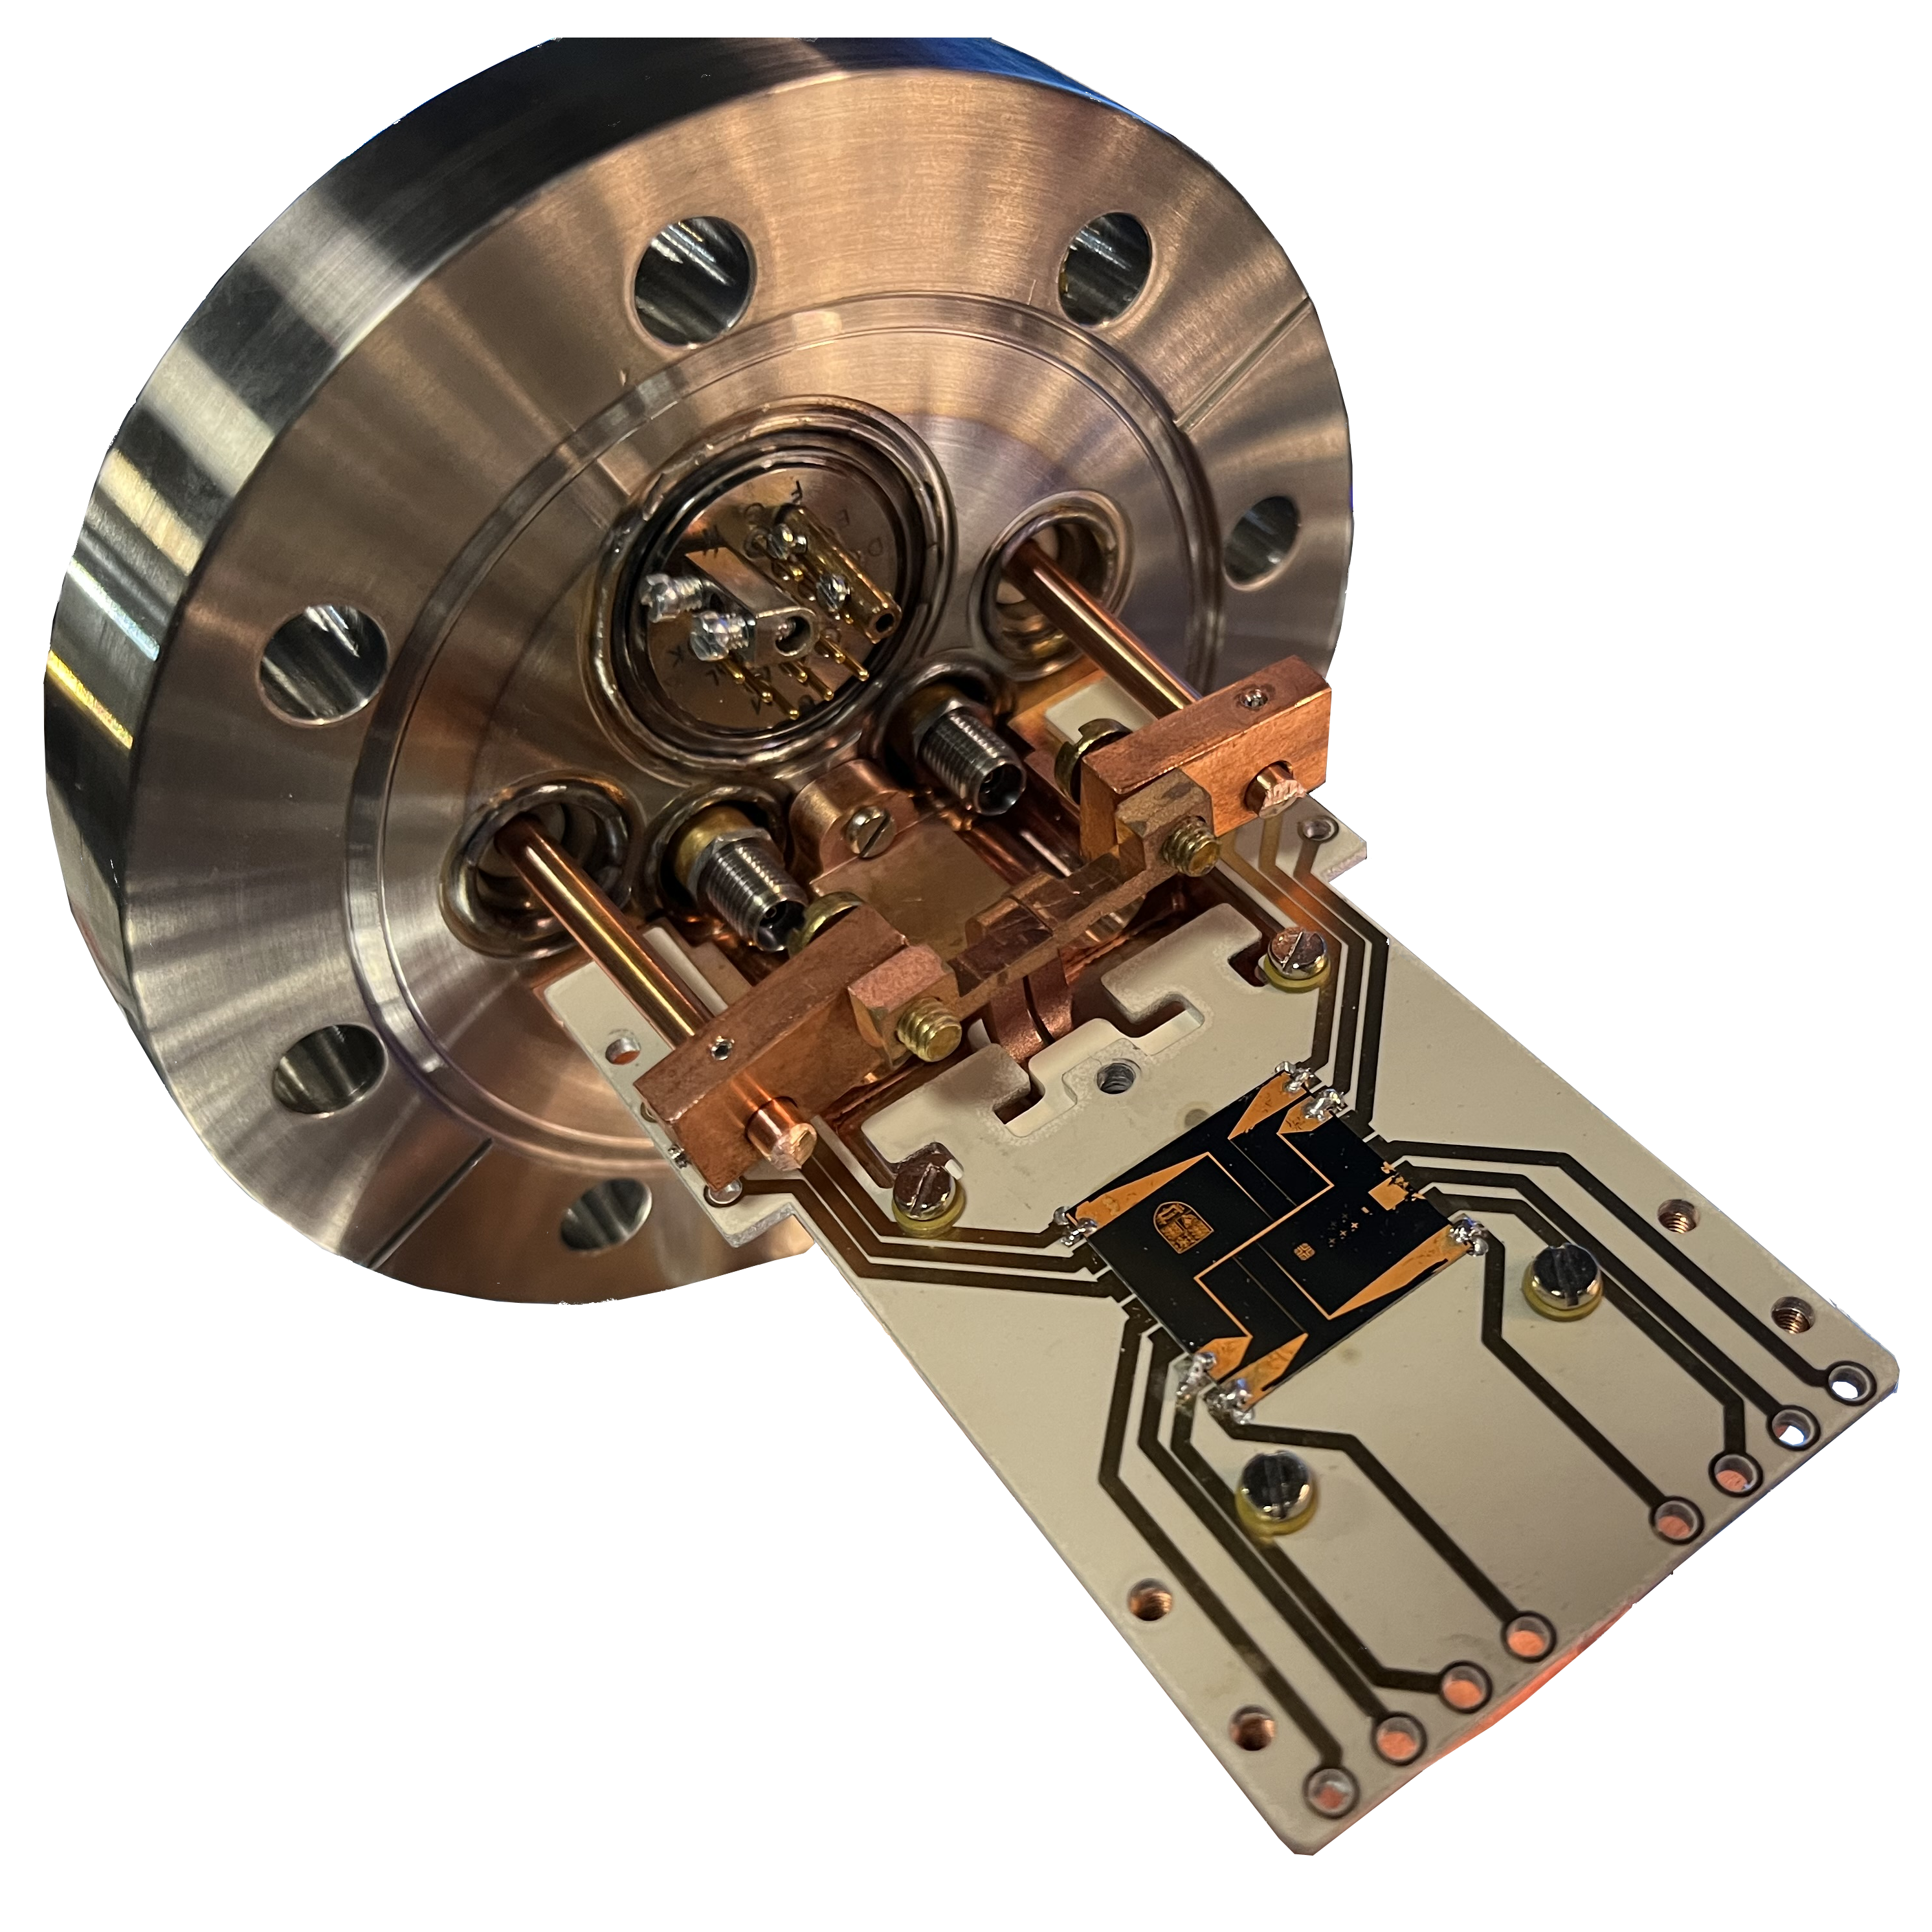
\includegraphics[width=\textwidth]{figs/chip_pic_crop.png}
    \caption{}
  \end{subfigure}
  \hspace{1cm}
  \begin{subfigure}[b]{0.45\textwidth}
    \centering
    %\includegraphics[width=\textwidth]{figs/chip_present2.pdf}
    \begin{overpic}[abs, width=\textwidth]{figs/chip_present4.pdf}
      \put(10, 160){\small (i)}
      \put(60, 160){\small(ii)}
      \put(175, 60){\small(iv)}
      \put(110, 137){\small(iii)}
      \put(70, 90){\small \SI{20}{\micro\meter}}
      \put(112, 93){\small\SI{10}{\micro\meter}}
      \put(8, 42){\small $\mathrm{Z_0}$}
      \put(8, 10){\small $\mathrm{Z_1}$}
      \put(8, 200){\small $\mathrm{Z_2}$}
    \end{overpic}
    \caption{}
  \end{subfigure}
  \caption{
    In (a) we have the chip assembly fully constructed, with a view of the
    aluminium-core PCB (subchip) for current delivery. Note also the polyimide
    bushings to electrically isolate the retaining screws from the surface. The
    microwave feedthroughs remain disconnected. In (b) we show a schematic of
    the chip features, with the scaling exaggerated for visibility. The three
    overlapping Z-wires are shown and labeled. The gaps between the wires are
    highlighted.
    %
    Toward the left (i) is the
    electroplating connection pad and various features used for
    characterisation (ii). On Z2 it is possible to see several small pads used
    as anchors, to secure the thin wire to the substrate.  The axis of the
    $\mathrm{Z1}$ wire is labeled for reference (iii) and the other wires are
    similar. All of the above features  will be discussed further in
    chapter~\ref{fab}. The crest of Imperial College London (iv) is also
    included.}
  \label{overview:fig:chipexperiment}
\end{figure}


The axial length of the wires also decreases to gradually reduce the size of
the trapped cloud in the $x$ direction. An exaggerated schematic of the wire
layout is shown in \myfigref{overview:fig:chipexperiment} and further details are
outlined in \mytableref{overview:table:wires}. All wires have been designed to
carry twice the current that is required in the loading scheme, so that there
is sufficient headroom for further experiments, and to reduce risk of
accidental damage to the chip during normal operation.

% TODO Maybe need more detail here
\begin{table}
  \centering
\begin{tabular}{lrrrrr}
  Name & Axis length (\si{\milli\meter}) & Width (\si{\micro\meter})& $I_\text{max}$ & Trap height (\si{\micro\meter}) \\
 \hline
  U & 16 & N/A& 100 & 3000\\
  $\mathrm{Z0}$ & 12 & 200& 60& $3000\rightarrow1000$ \\
  $\mathrm{Z1}$ &  6 & 20& 6& $1000\rightarrow100$ \\
  $\mathrm{Z2}$ &  2 & 2& 0.6& $100\rightarrow10$ \\
 \hline
\end{tabular}
  \caption{Details on the wire dimensions, maximum current, and desired
  trapping heights. The wire design is shown in
  \mysubfigref{overview:fig:chipexperiment}{c}. Note that the U-wire current is
  limited by vacuum feedthroughs and not by the maximum current calculated by
  the wire dimensions.  The maximum currents have been designed for use at only
  50\% of their potential maximum ($I_\text{max}$).
  }
  \label{overview:table:wires}
\end{table}


\cm{Fix phrasing}
In order to incorporate microwave guides onto the chip. This can be
accomplished by adding an insulating layer on top of the wires, on to which we
can fabricate coplanar waveguides~\cite{1127105}. The flange has been designed
with microwave feedthroughs, so that microwaves can be launched onto the
subchip and carried to the chip via coplanar waveguides \cm{to be discussed in
a later chapter}.

Having broadly outlined the experiment, the rest of this chapter will justify
the design of the trapping wires by means of simulation and analysis
of the trapping potentials.



\chapter{Simulating the trap}
\label{sim}
%\input{chapters/sim}

\chapter{Microfabrication}
\label{fab}
%Fabrication of a chip has been an iterative process, where we have
simultaneously improved upon both the chip's design and our fabrication
techniques.
In this chapter I will present the progress that we have made in
learning how to build a chip trap, and how we plan to integrate a microwave
guide in future experiments. 

All the microfabrication techniques described below except for the
electroplating were undertaken at the London Centre for Nanotechnology (LCN). 

\section{Overview of the fabrication procedure}

% TODO I grabbed this Madou2002 citation from Treutlein, but I should ensure
% that it is legit
Our trap has been designed so that the size of the wires is small compared to
the size and height of the trapped cloud. As such trapping wires on the chip
are as small as \SI{3}{\micro\meter} in width. Such small features can be
produced using standard photolithography techniques~\cite{Madou2002}. However,
the maximum height of features produced in these procedures is usually of the
order \SI{100}{\nano\meter}.

% TODO Need to cite this $j$ number
We must ensure that the wires are capable of carrying the currents that are
outlined in chapter~\ref{design}.  Other experiments with two-layer atom chips
have reported a current density of $j=\SI{6E10}{\ampere\per\meter\squared}$ in
the trapping wires. For our wires this would require a minimum height of $h
\sim I w/j = \SI{1}{\ampere} \times
\SI{10}{\micro\meter}/\SI{6E10}{\ampere\per\meter\squared} \sim
\SI{1}{\micro\meter}$  to carry our trapping currents.This is much higher than
can be achieved with photolithography techniques.

To achieve the required height, we have used through-mask
electroplating~\cite{Ruythooren_2000}. First a substate is coated with a thin
seed layer of gold, then photolithography is used to produce a thick (several
mircron high) mould. The mould covers regions where no further deposition is
required. The substrate can then be electroplated, with the seed layer acting
as the anode, allowing thick wires to be deposited into the mould.
After electroplating the seed layer can be etched away. This is a common
technique for constructing atom chips and is described in \inlinerefs{2011Ac,
Lev2003, KOUKHARENKO2004600}.

The fabrication process for our final chip begins with a four inch silicon
wafer, which we dice into individual \SI{20}{\milli\meter} by
\SI{20}{\milli\meter} dies. The remaining process can be briefly summarised:
\cm{Is there a better way to link this list to the following sections?}
\begin{enumerate}
\item Lay down thin (\SI{60}{\nano\meter}) seed layer of chromium and gold.
\item Spin coat a thick (\SI{6}{\micro\meter}) layer of photoresist.
\item Expose and develop the thick photoresist so as to create a ``mould''
in the desired shape of the wires.
\item Electroplate the chip, such that wires are formed in the mould to the
desired height.
\item Remove the photoresist mould.
\item Chemically etch the chip so as to remove the seed layer and
  electrically isolate the wires.
\end{enumerate}
This process is illustrated in \myfigref{fab:fig:process}

\begin{figure}[h]
\vspace{0.8cm}
\centering
\begin{tabular}{cccc}
  %\begin{overpic}[width=0.22\textwidth]{figs/fab/cartoon/01_barewafer.pdf}
  %  \put(0,40){(a)}
  %\end{overpic} &
  \begin{overpic}[width=0.22\textwidth]{figs/fab/cartoon/03_wafercrauwarrows.pdf}
    \put(0,40){(1)}
  \end{overpic} &
  \begin{overpic}[width=0.22\textwidth]{figs/fab/cartoon/03.5_waferpr.pdf}
    \put(0,40){(2)}
  \end{overpic} &
  \begin{overpic}[width=0.22\textwidth]{figs/fab/cartoon/04_wafermould.pdf}
    \put(0,40){(3)}
  \end{overpic} \\[2cm]
  \begin{overpic}[width=0.22\textwidth]{figs/fab/cartoon/e.pdf}
    \put(0,40){(4)}
  \end{overpic} &
  \begin{overpic}[width=0.22\textwidth]{figs/fab/cartoon/f.pdf}
    \put(0,40){(5)}
  \end{overpic} &
  %\begin{overpic}[width=0.22\textwidth]{figs/fab/cartoon/g.pdf}
  %  \put(0,40){(g)}
  %\end{overpic} &
  \begin{overpic}[width=0.22\textwidth]{figs/fab/cartoon/h.pdf}
    \put(0,40){(6)}
  \end{overpic}
\end{tabular}
  \caption{
    Illustration of the fabrication process. We begin with in (1) with a
    silicon die (black), on which we deposit chromium adhesion layer (grey) and
    a seed layer of gold (yellow). In (2) the entire die is spin coated in
    photoresist (purple). The mould is formed by photolithography techniques
    (3) and then electroplating is used to form tall wires (4). The photoresist
    is removed (5), and then a gold etch followed by a chrome etch (6) are used
    to electronically isolate the features.
  }
  \label{fab:fig:process}
\end{figure}

As discussed in chapter~\ref{intro}, a future aim of the molecule chip project is to
integrate microwave guides on the chip. These guides must allow good overlap of
the microwave fields and the molecule trapping region. Our design achieves this
by positioning the microwave guides on a second layer, directly above the
trapping wires. We have not yet attempted the following stages of
fabrication, but we anticipate that they will be:
\begin{enumerate}[resume]
    \item Spin coat chip with an insulating layer of polyimide.
    \item Perform standard photolithography to lay down microwave guides on the
      chip.
\end{enumerate}
These steps are discussed further in section~\ref{fab:planned}.

In the rest of this chapter I will describe the above process in detail,
including the various pitfalls that we found as we itterated towards a complete
\cm{trapping chip}.

\section{Metal evaporation of seed layer}

Before any fabrication, the die must be cleaned and dehydrated to ensure that
there will be good adhesion to the substrate. A solvent clean with acetone and
isopropyl alchol will remove any organic compounds \cm{check this}. The die is
then rinsed with deionised water and dehydrated in an oxygen plasma for ten
minutes.

The die is then ready for metalization, which here is done by metal
evaporation. To further improve adhesion between the gold and silicon, a thin
($<10\si{\micro\meter}$) intermediary chrome layer is deposited first, followed
by \SI{50}{\micro\meter} of gold.

We performed evaporation using an Edwards A306 bell jar evaporator. Typically
we \cm{metalize} four dies at a time. They are loaded into the belljar, along
with gold and chrome, using a boat and rod respectively.  we deposit gold onto
four dies at a time. The dies are positioned with the polished side facing down
towards the metal. This arrangement is shown in \myfigref{fab:fig:belljar}.

\begin{figure}
  \centering
  \ph{Photo of bell jar with evaporation and layout cartoon}
  \caption{\ph{caption}}
  \label{fab:fig:belljar}
\end{figure}

The belljar is pumped down to pressures below $10^{-6}\si{\milli\bar}$ over a
few hours. The metal for deposition can be selected from a carousel, and heated
by electric current inducing evaporation.  A shutter is used to block
deposition onto the substrate until the desired current has been reached.

The Edwards bell jar evaporator incorporates a FTM7 deposition monitor, which
reports the rate of deposition and automatically shuts off deposition once the
desired thickness has been reached by closing the shutter. \cm{What
determines/ limits the deposition rates? What happens when we have too much
current?}

The deposition rate of gold is typically \SI{0.2}{\nano\meter\per\second}.
%
\cm{Find a way to cite LCN for this and maybe some other factoids.}
%
As discussed above a thickness of \SI{5}{\micro\meter} is desirable for the
chip's trapping wires. Achieving this with evaporation would take over an hour,
and it would not be possible to load the evaporator with enough gold to last
this long. This is why we must use electroplating to achieve the desired
thickness.

\section{Spin coating of photoresist}
\label{fab:spin}

Spin coating is a procedure for distributing a uniform layer of liquid such as
photoresist  across a substrate~\cite{Cohen2011}. It is typically followed by
baking to solidify the layer. We use spin coating to apply SPR220-7 \cite{}
photoresist, which will form the mould for the wires.

The die is mounted in the \cm{spin coater details}, and \cm{how much? I can
check pippete...} of SPR220-7 is applied. The die undergoes a
\cm{\SI{2}{\second} ramp to \SI{500}{\rpm} where it is held before a ?second
ramp to \SI{4000}{\rpm} and held for \SI{30}{\second}.} This results in a
nominal \SI{6}{\micro\meter} high coating of photoresist \cm{according to LCN,
but we haven't actually varified this}.
SPR220-7 requires a post-application bake, first at \SI{90}{\celsius} for two
minutes, then immediately afterwards at \SI{120}{\celsius}.

Spin coating the photoresist results in a bead at the edge of the die. This
thick region of photoresist may not receive sufficient exposure to fully
develop later. This can cause defects in features near the edge. It is
possible to remove the bead by inserting an intial exposure and development
step before the lithography discussed in the next section. However, since the
only features that are covered by the bead are the robust wire bond pads, this
is deemed unnecessary for our purposes. \cm{Defects due to the presence of a
bead can be seen in \myfigref{}.}

\section{Lithography of the wire mould}

Lithography is the process of projecting the image of a design onto the surface
of the substrate. The usual procedure is to coat the substrate in a
photoresist, which can be exposed to ultraviolet light. In our case, SPR220-7
is a positive photoresist, meaning that exposed regions of the
photoresist can be removed from the wafer by submersion in a suitable
photoresist developer. Here, \cm{find name!} was used. 

The common and, perhaps, traditional way to perform photolithography is to use
a \cm{mercury} lamp and a chrome-on-glass mask to cast light onto the
substrate, with the mask casting a shadow so as to illuminate only the desired
region~\cite{Madou2002}. This was the method that we began using at the start of the
project, however we found that it was easier to achieve reliable results by
using the the Heidlberg DWL 66, a direct writer~\cite{}. 

Instead of using a mask to cast a shadow, the direct writer uses a tightly
focused ultraviolet laser, whose beam is raster scanned across the surface. The
beam is then switched on and off so as to produce the pattern that is required.
This process is depicted for a in \myfigref{fab:fig:methods}. The Heidelberg
DWL 66 is capable of producing features down to \SI{300}{\nano\meter} in size.
For SPR220-7 an exposure energy of \cm{??} is required, which is administered
over three passes of the laser at \cm{intensity}. The whole scan for one die
takes around twenty minutes.

Since designs can be directly uploaded to the direct writer, there is no need
to wait for a third party to construct a mask.  Hence the direct writer allows
rapid prototyping. It also has the benefit of making alignment easier, since
this can be performed automatically by the computer, and any issues with
mask-die contact are avoided entirely.


\begin{figure}[h]
\vspace{0.8cm}
\centering
  \begin{overpic}[width=0.8\textwidth]{figs/fab/cartoon/throughmask.pdf}
    \put(10,-5){(a)}
    \put(35,-5){(b)}
    \put(61,-5){(c)}
    \put(86,-5){(d)}
    \put(-1,6){$h$}
    \put(23.2,-0.4){$x$}
  \end{overpic}
  \vspace{10mm}
  \caption{An illustration of how lithography is used to produce tall wires in
  through-mask electroplating. The top row shows a top-down view of the die,
  with a cross section along the dashed line shown in the middle row. The
  bottom row shows a profile of the target (as discussed in
  section~\ref{fab:inspmould}). Column (a) shows photoresist (purple) above the
  seed layer (\cm{colours as in \myfigref{}}) with the exposed region
  highlighted (light blue). The raster scan of the direct writer laser across
  the substrate is highlighted in the top view.  In column (b) the resist is
  developed and the seed layer is exposed. In column (c) gold is deposited via
  electroplating (as discussed in section~\ref{fab:eplate}) to just below the
  height of the mould. In column (d) the photoresist is removed, leaving the
  tall wires (highlighted with black outline) and seed layers, the latter of
  which will be removed by etching.
  }
  \label{fab:fig:tmep}
\end{figure}


This photoresist requires a rehydration step after exposure, so it is left at
ambient temperature overnight before it is developed with  \cm{what? for how
long?}. \cm{Reference first side-on fig.}


\subsection{Inspecting the photoresist mould}
\label{fab:inspmould}

\cm{Profiling, with examples and contact testing of the wire bond pads to
ensure no residue PR}

So far we have discussed the process up to the point that we have a photoresist
mould on top of the gold seed layer. The next step is to electroplate so as to
form the tall wires. However it is useful to first examine the mould so that we
can ensure any electroplating target is likely to produce a suitable chip.

The die can be imaged with a microscope for inspection of features. This is
useful to give an overview of key areas, and can be used to identify any
regions with potential defects. When these are identified it is often useful to
be able to examine the contours of the region.

This can be achieved with a stylus profilometer, such as the Bruker DektakXT
which was used here. A stylus profilometer operates by positioning a gold
stylus onto the surface of the die and dragging it in one direction. As
the stylus comes into contact with features its height will change, allowing a
profile of the surface to be measured. Profiling of a surface is illustrated
in the lowest row of \myfigref{fab:fig:tmep}

% TODO
% A typical example...

% Some common problems...

% Show the one that I developed again to make sure the mould was celar (this
% was a lettered chip)

%An example of the profile of a substrate
%is given for different stages of the lithography process in
%\myfigref{fab:fig:methods}. The Bruker Dektak allows profiling over a wide
%range of feature sizes, from \SI{1}{\nano\meter} to \SI{1}{\milli\meter}, and
%so is well suited to profiling our chips.
%%
%\cm{Figure out how to cite this}.
%
%\cm{Maybe some raster scans?}
%
%\cm{Profilometer results pls}
%
%The wafer is then diced and the individual chips are ready to be electroplated.


\section{Electroplating the tall wires}

Now the chip is returned to the Blacket Laboratory for electroplating.
Electroplating does not take place in cleanroom conditions, but it is important
that the dies are treated with great care during transport, and kept sealed
until electroplating can begin. We found that the dies were surprisingly
robust, and were able to be kept for several weeks between exposure and
electroplating.

In electroplating a conductive target (here, the die) is connected to an
electric circuit as an anode and placed into an electrolytic solution along
with a cathode. Current passed through the solution causes ions in the solution
to be deposited onto the target. This is illustrated in
\mysubfigref{fab:fig:etch}{a}. An overview of electroplating can be found in
\inlineref{Schlesinger2011}.
%
\cm{This ref again, check it is ok!}

Here we use the through-mask electroplating method to deposit thick gold wires
into the regions that are not covered by the photoresist mould, as shown in
\myfigref{fab:fig:eplate}. This method allows us to produce wires up to the
thickness of the photoresist height. Above this the wires will begin to
``mushroom,'' spreading out across the top of the photoresist and losing their
shape. As per the discussion in \cm{ref chapter}, we require a minimum wire
height of \cm{\SI{5}{\micro\meter}}. We will see below that we have been able
to reliably produce wires up to a height of \SI{6}{\micro\meter}.

\cm{include photo of apparatus}
%
\begin{figure}
\vspace{0.8cm}
\centering
  \begin{overpic}[width=0.22\textwidth]{figs/fab/cartoon/eplate.pdf}
    \put(-10,100){(a)}
    \put(28.7,91.2){$I$}
  \end{overpic}
  \caption{
    A chip (c.f.\myfigref{fab:fig:prep}) is submerged in a gold electrolyte
    (light blue) along with an electrode (grey mesh). These are connected to a
    current supply to enable current flow and deposition of gold ions (yellow
    circle)  is depicted. The solution is held at \SI{58}{\celsius} and
    agitated by a stirrer and bubbler.
  %Subfigure (b) shows a photograph of our apparatus. A beaker
  %containing the electrolyte is placed in a water bath for heating during the
  %procedure.
  }
  \label{fab:fig:eplate}
\end{figure}

The height $h$ achieved in a deposition of duration $t$ is given by the Faraday
equation~\cite{Ruythooren_2000}
%
\begin{equation}
  h = \left(\frac{\alpha I M}{nFA\rho}\right)t
\end{equation}
%
where $I$ is the current, $F=\SI{96.5}{\kilo\ampere\second\per\mole}$ is the
Faraday constant, and other parameters with values specific to our gold
deposition are: $\alpha\sim0.9$, the current efficiency; $M =
\SI{197}{\gram\per\mole}$ the molar mass;
$\rho=\SI{19.32}{\gram\per\centi\meter\cubed}$, the density of the deposited
metal; $n=1$, the charge on the deposited ions in units of electron charge; and
$A\sim\SI{1}{\centi\meter\squared}$ is the area for plating.

We therefore have a relationship between the current, the target height and the
time,
%
\begin{equation}
  h \approx \left(
  \SI[per-mode=fraction]{1e-10}{\meter\cubed\per\ampere\per\second} \right)
  \times\frac{It}{A}.
\end{equation}
%
\cm{Ensure I am not word stealing here...}
For our electrolytic solution, we have used Metakem Goldbath-SF.
Metakem Goldbath-SF is chosen because it produces very pure (99.99\%) deposits,
and will not react with our photoresist. The effectiveness of this product has
been demonstrated for a similar design in \inlineref{Treutlein2008}.
%
\cm{Should cite metakem}

Goldbath-SF is suitable for use with current densities in the range
\SIrange{1}{15}{\milli\ampere\per\centi\meter\squared}. Final chip design has a
plating surface area of $S\approx85\si{\milli\meter\squared}$. There is also an
additional contribution to surface area from the clip with which we hold the
die in place during plating. We do therefore do not know the plating area
exactly, but we ensure that the entire clip in the solution every time to
ensure the results are reproducable. We can also estimate the minimum plating
time for wire heights of \SI{3}{\micro\meter}, which we expect to be
\cm{TODO}.

% Can we figure out the chip area from the offset of different plating times?

Our apparatus for the electroplating step is shown in
\mysubfigref{fab:fig:eplate}. The electrolytic solution is placed in a
beaker, which itself is placed in a water bath held at \SI{60}{\celsius}. The
bath is heated using a hotplate with magnetic stirrer. Some time is allowed for
thermalisation, during which it is imporant that the goldbath is covered to
prevent loss by evaporation.

When the goldbath has reached \SI{60}{\celsius} the target chip and the cathode
are submerged. The chip is held in position by a stiff insulated wire, which
also carries current to the seed layer. A multimeter can be used to ensure that
there is good electrical contact from the wire to the holder. The wire is
insulated, and we use the smallest clip possible so as to minimise gold plating
to the chip.  The cathode is a grid of platinised titanium which has been cut
to the size of our beaker.  This was also purchased from Metakem.

% Change this to show that electroplating without the aggitation didn't work
% The whole of the next three paragraphs needs to be turned into more of the
% narative of how we learned to electroplate. Including profiling results

A bubbler is placed to agitate the solution near to the chip surface. This in
combination with gentle stirring ensures good circulation of the solution and
hence prevents localised depletion of the ions near to the chip
surface~\cite{Schlesinger2011} \cm{also cite conversation with S Etienne?}.

After electroplating, dies are rinsed with deionised water, and the photoresist
is removed overnight with \cm{Dupont 1165 photoresist remover}.  Dies are then
dried and stored for transport to the LCN cleanroom for the inspection and
final fabrication steps.

We determined experimentally that electroplating at $\SI{15}{\milli\ampere}$
for duration $\SI{400}{\second}$ reliably produced wires of height
\SI{5}{\micro\meter} above the seed layer. This can be confirmed by profiling
the surface as described in section~\ref{fab:profile}, and can be undertaken
before and after the removal of the photoresist mould. 
%
\cm{Profile}

\subsection{Troubleshooting}

Building and running an electroplating setup was by far the most challenging
stage of the fabrication process. It is therefore worth noting some of the
complications that we experienced and how they were overcome.

% Doesn't work without aggitation

% Poor plating if the chip doesn't face the cathode (is this definitely a
% thing? I think I need a photo to be able to talk about this) plates only at
% edges

% Comparison between wires is hard, hence the new characterisation features

% Using a large crocodile clip seems to cause localised depletion (need to
% confirm this)

% Trying to remove with IPA and acetone instead of PR remover can cause debris

% Shadowing, as in Treutlein, with profiles and pictures

% Inconsistent heights when changing to fresh solution in order to resolve the
% shadowing (maybe a change in the efficency alpha between solutions??) I can
% show some plots for this too

\section{Photoresist liftoff and etching}

\cm{probably separate thes into two}

After electroplating the photoresist mould is removed with Microposit Remover
1165 as described in section~\ref{fab:prep}. The chip is now as pictured in
\myfigref{fab:fig:etch}{b}, with wires formed to the desired heights but all
connected electrically through the seed layer. The next step is to etch the
seed layer and the adhesion layer so that the wires are separated.

\begin{figure}[h]
\vspace{0.8cm}
\centering
\begin{tabular}{cccc}
\end{tabular}
  \caption{Cross section of the cleaning and etching of the chips following
  electroplating.  The electroplated chip (a) is cleaned to remove the
  photoresist layer (b). A gold etch (c) is performed, followed by a chromium
  etch (d) to produce electrically isolated wires. Colours are as in
  \myfigref{fab:fig:prep}.}
  \label{fab:fig:etch}
\end{figure}

\cm{Need to figure out the actual name of the etchant}
%
The gold etch is performed by placing the chip into a beaker of Iodine etchant,
which etches gold at a rate of \SI{5}{\nano\meter\per\second}. This means that
an etch of \SI{10}{\second} will remove the seed layer. After this the chip is
immediately transferred to a beaker of deionised water and then rinsed. Since
the seed layer thickness is significantly smaller than the dimensions of the
wire, the cross-sectional area will not be significantly altered in this time.
This can be confirmed with profiling (see below). At this stage the chip is as
picture in \mysubfigref{fab:fig:etch}{c}.

\cm{Need to find out what the Cr etchant is called}
%
To complete the separation of the wires, the chromium layer must also be etched
in the same way. The process is the same as for the gold etch: the chip is
submerged in a beaker of the etchant and after the pre-determined exposure time
it is transferred to deionised water and then rinsed. This stage of the
fabrication is represented in \mysubfigref{fab:fig:etch}{d}. 

To ensure that the etches have been successful, stylus profiling is once again
performed, results are shown in \myfigref{fab:fig:endprofile}. We ensure that
the wires are of a sufficient height and width to achieve the required currents
as detailed in chapter~\ref{design}. Visual inspection under an optical
microscope is also useful to ensure that the silicon has been completely
exposed. A multimeter is used to confirm that there are no breaks in the wires.



\begin{figure}
\centering
  \includegraphics[width=0.8\textwidth]{figs/fab/wire_profile.pdf}
  \caption{A profile of trapping wires after etching, showing wires
  electroplated up to a height of approximately \SI{3}{\micro\meter}.
  \cm{Mike says I need to make a better version of this figure. This is on my
  todos, but I really want to do it for the new chip design.}
  }
  \label{fab:fig:endprofile}
\end{figure}

\section{Scaling fabrication}

In future design iterations it may be useful to scale the fabrication process
up by fabricating on the wafer scale rather than the scale of an individual
die. An entire wafer can be metallised, be spin coated and exposed to
produce the photoresist mask. Electroplating on the wafer scale may prove to be
more complicated than our comparatively small targets, but \cm{...}

\section{Planned fabrication of microwave layer}
\label{fab:planned}

In chapter~\ref{intro} 
we described how a molecule chip could allow strong coupling between \CaF{}
molecules and a microwave field, however for this to be possible there must be
good overlap between the microwave field and the trapped
molecules~\cite{Andre2006}.
%
\cm{better cite needed maybe?}

This overlap has previously been achieved for atoms in a magnetic
trap~\cite{Treutlein2008}. An insulating layer is spin-coated onto the trapping
wires so that a CPW \cm{In final version I need to check that first use of
abbreviation is explained.} can be fabricated by
photolithography. The trap centre can be positioned in the region where the
microwave field is strongest. This has potential to allow coherent control of
the molecules and potentially even sideband cooling into the motional ground
state~\cite{Andre2006}.
%
\cm{more discussion elsewhere?}

We will develop our fabrication procedure further so that we can produce such a
chip. The first stage will be to spin coat the insulating layer on top of an
etched chip, as shown in \mysubfigref{fab:fig:cpw}{a}. Again taking our lead
from \inlineref{Treutlein2008}, we will use polyimide. Polyimide is chosen due
to its low dielectric loss tangent ($\tan\delta_e = 0.016$) which will minimise
conductor losses in the waveguide~\cite{Collin2007, Simons2004}.
\footnote{Although a suitable dielectric is
important to minimise conductor losses in a CPW, this chip will operate at room
temperature and so radiation losses will dominate. This was discussed in detail
in the early stage assessment and will not be repeated here.}
%
\cm{This \emph{will} be repeated in the thesis so I can link this better.}

When spin coating the polyimide it is essential that we are able to produce a
flat surface onto which we can fabricate the microwave layer. We can do this by
applying multiple layers of polyimide on the spin coater, so that any bumps are
smoothed out. This is known as planarisation and is discussed further in
\inlineref{Treutlein2008}.

\begin{figure}[h]
\vspace{0.8cm}
\centering
\begin{tabular}{cc}
  \begin{overpic}[width=0.22\textwidth]{figs/fab/cartoon/i.pdf}
    \put(0,40){(a)}
  \end{overpic} &
  \begin{overpic}[width=0.22\textwidth]{figs/fab/cartoon/j.pdf}
    \put(0,40){(b)}
  \end{overpic}
\end{tabular}
  \caption{Cross section of the fabrication of a two-layer chip. A layer of
  polyimide (teal) is applied to the chip. This insulating
  layer is shown in (a). Note that in this simplified illustration
  planarisation effects are ignored, and the surface may not be completely
  even. This is discussed further in the body text.
  The CPW wires can be fabricated on top of the polyimide (b) by evaporation.
  }
  \label{fab:fig:cpw}
\end{figure}

After the application of a planarised polyimide layer it will be possible to
fabricate microwave guides on the surface by lithography. The end result is
shown in \mysubfigref{fab:fig:cpw}{b}. We will undertake
further work to determine the required height of the CPW features and where
they must be positioned relative to the wires to achieve the strongest
coupling.


\chapter{Experiment}
\label{experiment}

\chapter{Coupling \CaF{} to on-chip microwaves}
\label{mws}
%% TODO Better intro spiel
\cm{
In chapter (probably the introduction) I introduced the concept of microwave
guides integrated into chip traps. Previous experiments have used on-chip
microave guides to couple to \cm{(I think this is right)} the hyperfine structure
of atoms. However, the coupling to heteronuclear dipolar molecules is much
stronger \cm{Why?}. In the strong coupling regime it may be possible to \cm{(do
cavity QED, sideband cooling, etc...)}
%
Need to briefly say that we will use the stretched states, but the detail on
this comes later.
}

\section{The coplanar waveguide}

The coplanar waveguide (CPW) was originally proposed by Cheng P.~Wen as a means
of guiding microwaves across the surface of a dielectric
substrate~\cite{1127105}. It consists of a central conductor with a ground
plane on either side, as pictured in~\myfigref{mws:fig:CPW}. CPWs have become
prolific, since they allow the creation of robust microwave devices, and offer
some benefits over other waveguide architectures, such as the stripline
waveguide, because they can provide circularly polarised fields, and also
provide easy access to the ground plane for shunt connections.

The CPW's geometry is defined by the centre conductor width ($S$) and the
channel width ($W$). The height of the conductor is $t$ and the dielectric
height is $h$.  The geometry of the CPW determines the region the microwave
field occupies, as illustrated in \myfigref{experiment:fig:CPWfield}.  The CPW
can therefore be designed to maximise overlap between the microwave field and a
cloud of molecules trapped nearby.  As a rough approximation the molecules
should be trapped at a distance $h\sim S$ above the centre of the CPW to
achieve a good overlap.~\cite{Boehi2009} The field surrounding the CPW is shown
in \mysubfigref{mws:fig:CPW}{b}, the equations defining this field can be found
analytically~\cite{Simons2004}, or the field can be determined by a
finite-element simulation.

\begin{figure}[ht]
  \centering
  \begin{subfigure}[b]{0.45\textwidth}
    \begin{overpic}[abs, width=\textwidth]{figs/mws/CPW_dims.pdf}
      \put(20, 180){(a)}
      \put(100, 25){$S$}
      \put(126, 12){$W$}
      \put(15, 43){$h$}
      \put(193, 58){$t$}
      \put(40, 43){$\epsilon_r$}
    \end{overpic}
  \end{subfigure}
  \begin{subfigure}[b]{0.45\textwidth}
    \begin{overpic}[abs, width=\textwidth]{figs/mws/CPWMode_legend.png}
      \put(20, 180){\textcolor{white}{(b)}}
      \put(165, 180){\textcolor{white}{High}}
      \put(165, 110){\textcolor{white}{Low}}
		  \put(20, 20){\textcolor{white}{\SI{20}{\micro\meter}}}
    \end{overpic}
  \end{subfigure}
	\caption{Subfigure (a) shows a perspective view of a segment of CPW on dielectric substrate, with
pertinent geometry and dielectric constants labeled. The conductor is in gold
  and the dielectric is left transparent. A COMSOL finite-element simulation of the
resulting field density near such a CPW is shown in (b), with
$S=\SI{20}{\micro\meter}$, $W=\SI{10}{\micro\meter}$, $\epsilon_r=10$,
$h=\SI{10}{\micro\meter}$. Conductor regions are highlighted in gold and the
end of the bottom of the substrate is marked with the black line. The field is
presented in arbitrary units to illustrate where strong coupling can be
achieved. Note that in a resonator the field will depend on the position in the
longitudinal direction.}
	\label{mws:fig:CPW}
\end{figure}

\subsection{CPW properties}

We will now consider the electric properties of a CPW. These will largely
depend on the the planar geometry of the waveguide, which we express in terms
of the ratio~\cite{1127105, Simons2004}
%
\begin{equation}
  k_0 = \frac{S}{S+2W} = \sqrt{1-{k'_0}^2}
  \label{eqn:k0def}
\end{equation}
%
For a waveguide made of a material with conductivity $\sigma$
and permeability $\mu$ and propagating field with frequency $\omega$
there is a skin depth~\cite{Simons2004}
%
\begin{equation}
  \delta = \sqrt{\frac{2}{\omega\mu\sigma}}
\end{equation}
%
and skin effect surface resistance~\cite{Simons2004}
%
\begin{equation}
  R_s = \frac{1}{\sigma\delta}.
\end{equation}

Since the field of the CPW will pass through both the dielectric and the
surrounding air, the CPW's capacitance is the sum of the capacitance of each of
these two parts
%
\begin{equation}
  C_\text{CPW} = C_\text{dielectric} + C_\text{air}.
\end{equation}
%
The method of finding these individual contributions is somewhat involved, so
we simply state the results here in terms of the elliptic integral of the
first kind $K(k)$~\cite{Simons2004}. The capacitance due to the dielectric is
%
%
\begin{equation}
  C_\text{dielectric} = 2\epsilon_0(\epsilon_\text{r1}-1)\frac{K(k_0)}{K(k'_0)}
\end{equation}
%
and the capacitance of the air region is
%
\begin{equation}
  C_\text{air} = 4\epsilon_0 \frac{K(k_0)}{K(k'_0)}.
\end{equation}

We can use this to find the effective permittivity~\cite{Simons2004}
%
\begin{align}
  \epsilon_\text{eff} &= \frac{C_\text{dielectric}}{C_\text{air}} \\
    &= \frac{1+ \epsilon_\text{r1}}{2} \\
\end{align}
%
where we have assumed that we are in the limit of a thick dielectric layer ($h
\gg W$ so that most of the field density is inside the dielectric.
%
The phase velocity (using $c$ as the speed of light) is~\cite{Simons2004}
%
\begin{align}
  v_\text{ph} &= \frac{c}{\sqrt{\epsilon_\text{eff}}} \\
    &= \frac{c}{\sqrt{(1 + \epsilon_\text{r1})/2}}.
\end{align}

Now using the approximation~\cite{Collin2007}
$\sqrt{\mu_0/\epsilon_0}\approx120\pi\text{Ohms}$ we have the line
impedance~\cite{Simons2004}
\begin{align}
  Z_0 &= \frac{1}{C_\text{air} v_\text{ph}} \\
    &= \frac{30 \pi}{\sqrt{(\epsilon_\text{r1}+1)/2}} \frac{K(k_0)}{K(k'_0)}
    \text{Ohms}
    \label{mws:eqn:Z0}
\end{align}
Note that the impedance of the waveguide has dependence only on the geometry in
the form of the ratio $k_0$, and the relative permittivity of the
substrate.~\cite{Simons2004} This means that for any substrate we choose the
value of $k_0$ can be chosen to fix the impedance at the standard $Z_0 =
\SI{50}{\ohm}$.

Therefore as long as $k_0$ is held constant the CPW can be tapered to change the
size of the centre conductor, and hence control the region the field occupies.

\subsection{CPW attenuation}

The electric field inside a CPW evolves according to
%
\begin{equation}
  \widetilde{E}(z) = \widetilde{E}(0)e^{-\gamma z}.
  \label{mws:eqn:Eloss}
\end{equation}
%
where $\gamma = \alpha + i\beta$, $\beta = 2\pi / \lambda$ is the wave
number and $\alpha$ is the attenuation constant.~\cite{Simons2004}
Taking the absolute value, the amplitude falls off as
%
\begin{equation}
  E(z) = E(0)e^{-\alpha z}.
\end{equation}

There are two contributing terms to the attenuation constant
%
\begin{equation}
  \alpha = \alpha_d + \alpha_c,
\end{equation}
%
there are the contributions from dielectric and conductor respectively.
Negligible contributions from radiative losses are
neglected~\cite{Frankel1991}.  Bending losses can be neglected as long as
the radius of the bends are much larger than the wavelength of the propagating
wave. We must be mindful of this during design, since the typical wavelengths
for rotational transitions are on the order of centimeters.
We also do not consider the insertion loss of the resonator, since this does
not affect the quality factor~\cite{doi:10.1063/1.3010859}.

\subsubsection{Dielectric losses}

Dielectric losses in the thick dielectric limit are described
by ~\cite{Collin2007}
\begin{equation}
  \alpha_d =
  \frac{\omega_0}{4c}\frac{\epsilon_\mathrm{r1}}{\sqrt{\epsilon_\mathrm{eff}}}
  \tan \delta_e
\end{equation}
%
where $\tan\delta_e$ is the dielectric loss tangent. Common dielectrics for
microwave guides include aluminium nitride (\AlN{}) and high-resitivity
silicon.  For our purposes we wish to consider waveguides situated on
dielectrics layers that can be easily deposited above the trapping wires.
Following the work in \inlineref{Treutlein2008}, we primarily consider polyimide, which
can be despoitied by spoin-coating. Other options are available, such as
polyethylene naphthalate (PEN) ~\cite{WEI20169937}.

Typical values of dielectric constants and $\alpha_d$ are shown in
\mytableref{mws:table:diprops}. Note that these parameters have some dependence
on the frequency and temperature of the dielectric, and so are presented to
illustrate the amount of loss that can typically be expected for our experiment
at room temperature and frequencies in the \SI{10}{\giga\hertz} r\'egime.

% TODO Add arlon thing to dielectrics table
\begin{table}[ht]
  \caption{Dielectric constants and loss for various substrates in the
  \SI{10}{\giga\hertz} r\'egime at room temperature}
\centering
\begin{tabular}{l c c c c }
\hline\hline
  Material & $\epsilon_r$ & $\tan\delta_e$ & $\alpha_d$ (\si{\per\meter})& Ref. \\ [ 0.5ex]
\hline
  Polyimide & 3.4 & \SI{1.8E-2}{} & 0.45 & \cite{DuPontKapton} \\
  PEN & 2.56 & 0.003 & 0.63 & \cite{WEI20169937} \\
  Silicon (high resistivity)& $\sim{12}$ & \SI{2E-4}{} & 0.02 & \cite{Simons2004, 1717770, doi:10.1063/1.4929503} \\
  Sapphire & $\sim10$ & $2\times10^{-5}$ & $10^{-3}$ & \cite{mw101}\\ % TODO Better cite?
  Aluminium nitride & 8.9 & \SI{5E-4}{} & 0.22 & \cite{mw101} \\ % TODO Better cite?
\hline
\end{tabular}
\label{mws:table:diprops}
\end{table}

\subsubsection{Conductor losses}

Conductor losses arise due to dissipation in the centre conductor and ground
plane of the CPW~\cite{Simons2004}.
The conductor attenuation constant is
\begin{equation}
  \alpha_c = \frac{R_c +R_g}{2Z_0}.
\end{equation}
Where $R_c$ and $R_g$ are the series resistances of the centre conductor and
the ground plance respectively.
For a waveguide with height 
$t$, theses are given by
\begin{equation}
  R_c = \frac{R_s}{4 S(1-k_0^2)K^2(k_0)}\left[ \pi + \log\left(\frac{4\pi
  S}{t}\right) - k_0\log\left(\frac{1+k_0}{1-k_0}\right) \right],
\end{equation}
and
\begin{equation}
  R_g = \frac{k_0 R_s}{4S(1-k_0^2)K^2(k_0)}\left[\pi +
  \log\left(\frac{4\pi(S+2W)}{t}\right) -
  \frac{1}{k_0}\log\left(\frac{1+k_0}{1-k_0}\right)\right].
\end{equation}
%
The electrical properties of silver and gold are given in
\mytableref{mws:table:metalprops}, and the computed conductor attenuations are
shown in \myfigref{mws:fig:conductorloss}.

\begin{table}[ht]
  \caption{Electrical constants and loss for various conductors in the
  \SI{10}{\giga\hertz} r\'egime at room temperature}
\centering
\begin{tabular}{l c c c}
\hline\hline
  Material & $\sigma$ (\si{\siemens\per\meter}) & $\mu_r$ & Ref. \\ [ 0.5ex]
\hline
  Gold & & & \cite{} \\
  Silver & & & \cite{} \\
\hline
\end{tabular}
\label{mws:table:metalprops}
\end{table}

% Data generated by nbs/2022-02-06_CPWresonators.nb
\begin{figure}[h]
  \centering
  \begin{subfigure}[b]{0.48\textwidth}
  \begin{tikzpicture}
    \begin{axis}[
        xmode=log,
        enlargelimits=true,
        xlabel=$t$ (\si{\nano\meter}),
        ylabel=$\alpha_c$ (\si{\neper\per\meter}),
        width=\textwidth,
        height = 0.7\textwidth,
        x tick label style={/pgf/number format/.cd, set thousands separator={}}
    ]
      \addplot [thick, black] table {figs/mws/conductorlossvaryt.dat};
      \addplot [style=thick, color=blue] table [y index=2] {figs/mws/conductorlossvaryt.dat};
      \addplot [style=thick, color=pink] table [y index=3] {figs/mws/conductorlossvaryt.dat};
      \node [] at (5cm, 3.1cm) {(a)};
    \end{axis}
  \end{tikzpicture}
  \end{subfigure}
  \begin{subfigure}[b]{0.48\textwidth}
  \begin{tikzpicture}
    \begin{axis}[
        enlargelimits=true,
        xlabel=$S$ (\si{\micro\meter}),
        %ylabel=$\alpha_c$ (\si{\neper\per\meter}),
        width=\textwidth,
        height = 0.7\textwidth,
        x tick label style={/pgf/number format/.cd, set thousands separator={}}
    ]
      \addplot [thick, black] table {figs/mws/conductorlossvarys.dat};
      \addplot [style=thick, color=blue] table [y index=2] {figs/mws/conductorlossvarys.dat};
      \addplot [style=thick, color=pink] table [y index=3] {figs/mws/conductorlossvarys.dat};
      \node [] at (5cm, 3.1cm) {(b)};
    \end{axis}
  \end{tikzpicture}
  \end{subfigure}
    \caption{
      Conductor losses are plotted for (a) varying the conductor height of the
      CPW and (b) varying the centre conductor width. Losses are shown for gold
      on sapphire (black), silver on sapphire (blue) and gold on polyiide
      (red). In (a) a typical conductor width of $S=\SI{10}{\micro\meter}$ is
      assumed, and in (b) the thickness of the conductors is taken to be
      $t=\SI{5}{\micro\meter}$. In both cases the impedance is set to $Z_0 =
      \SI{50}{\ohm}$ by choice $k_0$ by \myeqref{mws:eqn:Z0}.
    }
  \label{mws:fig:conductorloss}
\end{figure}

The conductor losses clearly dominate over the dielectric losses. For this
reason it is common to use superconductors for CPWs~\cite{}, since for a
superconductor $\sigma \to \infty$ and hence $R_s$ and $\alpha_c \to 0$.
This will not prevent the implementation of a microwave guide on a multi-layer
chip trap, but it will impact our ability to build incorporate a microwave
resonator as we will now discuss.

That said, it should be noted that the high loss will not prevent the use of
the CPW to directly drive microwave transitions in trapped molecules. This
would allow the same coherent control achieved in free space
experiments~\cite{WilliamsMagnetic2018} although realisation of the JCH will
clearly not be possible and a strong driving field may be required to overcome
losses.  With loss of $\alpha \approx \alpha_c$, and waveguides of lengths on
the scale of a few centimeter, we can expect a total loss of around
$\SI{400}{\neper\per\metre} \times \SI{0.01}{\metre} = \SI{35}{\decibel}$. This
should be sufficiently small that microwaves will be able to reach molecules
trapped on the chip.~\cite{Treutlein2008}

\subsection{CPW resonators}
\label{mws:resonators}

A microwave resonator can be formed from a section of CPW that is capacitively
coupled to another driving segment~\cite{Day2003}. The resonant frequency is
determined by the resonator's length, $L$, and the waveguide's phase
veloctiy~\cite{Simons2004}
%
\begin{equation}
  \omega_0 = \frac{\pi v_\text{ph}}{L} = \frac{\pi
  c}{\sqrt{\epsilon_\text{eff}} L}
\end{equation}
%
Microwaves can be coupled to the resonator by positioning the resonator inline
with a microwave guide, or in parallel as shown in \cm{some figure that I need
to make}. The strength of the coupling can be controlled by the shape of the
interface between the resonator and the waveguide~\cite{doi:10.1063/1.3010859}

Recall from the discussion in chapter~\ref{theory} that for strong coupling we
require $Q > 1.7 \times 10^5$. The quality factors for CPW resonators can be
expressed in terms of an attenuation constant
%
\begin{equation}
  Q = \frac{\omega_0}{2c\alpha}.
  \label{mws:eqn:Qalpha}
\end{equation}
%
From \myfigref{mws:fig:conductorloss} and \mytableref{mws:table:diprops} it is
clear that without the use of superconductors, the attenuation will be
dominated by conductor losses, and $Q\sim10$. This is clearly not sufficient
for our purposes.

Conductor losses can be eliminated by use of a superconducting CPW. CPW
resonators are a developed technology, commonly used for coupling to
solid-state qubits~\cite{Wallraff2004}. Operating at the low temperatures
required for superconductors allows the achievement of very high quality
factors of order $10^6$~\cite{doi:10.1063/1.3552890, Day2003}. For such devices
a low-loss dielectric is usually chosen for the substrate (sapphire being a
common choice) however a multi-layer resonator could potentially be achieved by
etching the polyimide in the slot gaps, as in \inlineref{920142}. Otherwise, a
single-layer superconducting design such as that shown in
\inlineref{Hattermann2017} could be adopted. Regardless, the multilayer design
remains a useful tool for prototyping a \cm{strong-coupling experiment.}
\cm{Rephrase this to stress that it might still work with resonator.}

% I have this point from Goppl that at low drive powers Q is somehow reduced. I
% don't understand this really, and don't think it's that relevant because we
% are so far off single-photon regime here anyway. But didn't want to entirely
% forget, so now this comment exists.

\section{Implementation of CPW-molecule coupling}
\label{mws:integrating}

Having established the CPW, and that such a device can operate on a polyimide
substrate, we can now consider the logistics of implementing such a device
with our design. In this section we will consider the \cm{states that we will
use} and \cm{how the transition frequency can be tuned to (or away from) the
resonator frequency}. We have already outlined how to fabricate a multi-layer device
in chapter~\ref{fab}, but the problem of delivering microwaves to the CPW
will also be discussed in this section.

% TODO Ensure this is introduced
For the remainder of this chapter we will consider microwave coupling to the
$\omega_0 = 2\pi \times \SI{20.5}{\giga\hertz}$ transition between the
stretched states, which was introduced in section~\ref{theory:molecules}.

\subsection{Stark shift}

Since the resonant frequency of the resonator is fixed by its length, it will
be useful to be able to tune the frequency of the molecule transition, either
to bring the molecules into or out of resonance with the microwaves. We
propose that this can be done by using the Stark shift due to a d.c.~field.
By positioning voltage-biased pads near to the molecule trap, the d.c.~field
can be used to shift the transition frequency.

When the shift is sufficiently small compared to the unperturbed energy, the
Stark shift can be found by second-order perturbation theory. The full
derivation can be found in, for example \inlineref{}, but for our purposes it
is sufficient to simply state the result, which is that the energy shift of the
% TODO Where do I introduce this notation?
rotational state is $\ket{N, m_N}$ is given by
% TODO Where do I introduce this energy rot notation?
%
\begin{equation} \Delta_{N, m_N} = \sum_{N', m_N'} \frac{(\mu_e
E)^2}{E_\text{rot}(N) - E_\text{rot}(N')} |\bra{N', m_N'}C_0^{(1)} \ket{N,
m_N}|^2.  \end{equation}
%
Where $C_q^{(k)}$ is a renormalised spherical harmonic, and the matrix element
here can be found by application of the Wigner-Eckart theorem~\cite{}.
% TODO Cite Mike's thing and Edmonds textbook
%
\begin{equation} \bra{N', m_N'}C_0^{(1)} \ket{N, m_N} =
  (-1)^{m_N'}\sqrt{(2N+1)(2N'+1)}
  % 3 j symbols
  \begin{pmatrix} N' & 1 & N \\ -m_N' & 0 & m_N \end{pmatrix} \begin{pmatrix}
N' & 1 & N \\ 0 & 0 & 0 \end{pmatrix} \end{equation}
%
where the last two matrices represent the usual 3j-symbols.


The summation can be simplified when we note that the properties of 3j-symbols
mean that mixing only ocurrs between states where $m_N' = m_N$ and $N=N'$. It
is simple to compute the resulting energy shift for arbitrary states, and the
results are shown for $N=0, 1, 2$ \CaF{} states in \myfigref{mws:fig:stark}. We
note that for small field strengths it is possible to induce a transition shift
of several gigahertz with a modest electric field strength. We anticipate that
only shifts on the order of $<\SI{1}{\mega\hertz}$ will be required in
experiment, and for such small perturbations, any additional effects of mixing
hyperfine states, or effects due to the magnetic field can be ignored.

% Data generated by nbs/2022-02-16_stark.nb
\begin{figure}[h]
  \centering
  \begin{tikzpicture}
    \begin{axis}[
        enlargelimits=true,
        xlabel=Field strength ($B/\mu_e$),
        ylabel=State energy (\si{\giga\hertz}),
        width=0.7\textwidth,
        height = 0.4\textwidth,
        legend pos=outer north east
        %x tick label style={/pgf/number format/.cd, set thousands separator={}}
    ]
      \addplot [thick, black] table {figs/mws/stark.dat};
      \addlegendentry{$\ket{0,0}$}
      \addplot [style=thick, color=blue] table [y index=2] {figs/mws/stark.dat};
      \addlegendentry{$\ket{1,0}$}
      \addplot [style=thick, color=pink] table [y index=3] {figs/mws/stark.dat};
      \addlegendentry{$\ket{1,\pm1}$}
      \addplot [style=thick, color=purple] table [y index=4] {figs/mws/stark.dat};
      \addlegendentry{$\ket{2,0}$}
      \addplot [style=thick, color=gold] table [y index=5] {figs/mws/stark.dat};
      \addlegendentry{$\ket{2,\pm1}$}
      \addplot [style=thick, color=grey] table [y index=6] {figs/mws/stark.dat};
      \addlegendentry{$\ket{2,\pm2}$}
    \end{axis}
  \end{tikzpicture}
  \caption{The Stark effect for the rotational states of the molecule $\ket{N,
    m_N}$ found by second order perturbation theory. The $N=2$ state is
  included for completion.}
  \label{mws:fig:stark}
\end{figure}

\subsection{Integrating microwave components}

% COMPONENTS
% Vacuum-side barrel connector
% https://www.mouser.co.uk/ProductDetail/Radiall/R127703001?qs=exnfk7tZe0CIIzofDocGig%3D%3D
% Vacuum-side launcher
% https://www.pasternack.com/2.92mm-female-end-launch-pcb-connector-pe45507-p.aspx
% Feedthroughs
% Kyle wrote in one note it's MDC SMA45-GS-WELD 
% I can't quite find this, think the new version is this one
% https://www.mdcprecision.com/9251004-sma-coaxial-feedthrough-1-pin-grounded-shield-double-ended-weldable

The chip flange (shown in \myfigref{overview:figs:chipexperiment}) has been
designed to incorporate MCD Precision's SMA45-GS-WLED \SI{2.92}{\milli\meter}
high-frequency SMA feedthroughs. These welded connectors can be used to bring
microwaves inside the chip chamber, where they can be launched onto a CPW on
the subchip. Microwaves will be transfered through from the feedthrough to the
subchip using a SMA male-male barrel adapter from Pasternak, and a female-clamp
PCB launcher from Pasternack. The launching assembly can be seen in
\mysubfigref{mws:fig:implement}{a}. These components have been tested for UHV
compatability, as discussed in \cm{reference relevant chapter}.  The flange
assembly has been designed to allow microwaves to exit the chamber, where they
can be terminated or measured.

Once launched onto the subchip, the microwaves will be delivered by CPW to the
subchip. 
%
As discussed in chapter~\ref{} the subchip in its current form is \cm{an
aluminium-core PCB}, however in future iterations of the experiment this can be
replaced with, for example, an Arlon AD1000 board, which will be a suitable
carrier for both trapping currents and microwaves~\cite{Morgan2020}. 
%
The subchip CPW will be connected to the \cm{science chip} CPW by wire-bonds.
These can be chosen to be arbitrarily large s that it is easy to make good
connection with the wire bonds, and then tapered down to reduce the field size
while maintaining the same $k_0$ and hence the same impedance. This CPW can be
capacitively coupled to a microwave resonator, but for a simple example we show
a multi-layer design for a single CPW in \mysubfigref{mws:fig:implement}{b}.

\begin{figure}[htb]
    \centering
    \begin{tabular}[t]{cc}
\begin{subfigure}{0.4\textwidth}
    \centering
    \smallskip
    \begin{overpic}[abs,
      width=\textwidth]{figs/mws/FlangeAssemblyFinalMWPresent.png}
      \put(10, 132){(a)}
    \end{overpic}
\end{subfigure}
    &
        \begin{tabular}{c}% if you add [t], than sub images are pushed down
        \smallskip
            \begin{subfigure}[t]{0.4\textwidth}
                \centering
                \begin{overpic}[abs, width=0.8\linewidth]{figs/mws/present_CPW2_IS.pdf}
                  \put(5, 139){(b)}
                \end{overpic}
            \end{subfigure}\\
            \begin{subfigure}[t]{0.4\textwidth}
                \centering
                \begin{overpic}[abs, width=0.8\textwidth]{figs/mws/present_CPW2_inset.pdf}
                  \put(5, 139){(c)}
                \end{overpic}
            \end{subfigure}
        \end{tabular}\\
    \end{tabular}
  \caption{
    The microwave components of the flange assembly (flange, feedthroughs,
    barallel connectors, launchers, PCB and chip) are shown in (a). In (b) we
    have the chip design from \myfigref{overview:figs:chipexperiment} (not to
    scale) with the
    additional microwave guide layer overlayed (red). Conversely to the lower
    layer, the microwave layer shows areas where the dielectric is exposed, so
    regions that aren't pink are covered with conductor. Example voltage pads
    for Stark-shifting the molecules are also shown. Subfigure (c) shows a
    detailed view of the trapping region.
  }
  \label{mws:fig:implement}
\end{figure}


To form an even smaller trap than discussed above, the CPW centre conductor can
be biased, to create a dimple trap along with the underlying axis of the
Z-wire, as was done in \inlineref{Treutlein2008}. For a resonator it would also
be possible to introduce a bias field, but this would have to be done on-chip
with a band stop filter~\cite{doi:10.1063/1.4808364}. This could also be used
to implement the electrostatic traps described in \inlineref{Andre2006}.

\section{Sideband cooling}

This subsection summarises the sideband cooling scheme presented in
\inlineref{Andre2006} and presents cooling rates for our trapping scheme with
\CaF{}.  Throughout section we assume that we operate with a single molecule
coupled to a high-quality cavity ($Q\sim10^6$, $\kappa \approx
2\pi\times \SI{20}{\kilo\hertz}$) in the
strong coupling r\'egime ($g\sim10^5>Q$)

In the macroscopic magnetic trap, the
$\ket{e}\rightarrow\ket{g}$ decay is very slow ($\Gamma \sim
10^{-5}\si{hertz}$), but when a molecule is in close proximity to a microwave
resonator at the transition frequency, the decay rate is strongly enhanced. 
with rate
%
\begin{equation}
  \Gamma_c = \frac{\kappa}{2}.
\end{equation}

This enhanced decay rate opens the door to sideband cooling into the motional
ground state of the trap.
%
We write the state of the molecule as $\ket{N, m}$ where $N\in\{e,g\}$ is the
rotational state of the molecule, and $m$ is the quantum number of the motion
in the trap. For any ground state $\ket{g,m}$ there is a carrier frequency
transition to $\ket{e, m}$ at the resonant frequency $\omega_0$, and sidebands
to the $\ket{e, m+m'}$ states at frequency $\omega_0 + m'\omega_t$, where
$\omega_t$ is the trap frequency and $m'\in \mathbb{Z}$. There are similar
carrier and sideband transitions for $\ket{e,m} \rightarrow \ket{g, m+m'}$.

We imagine that an external driving field is applied on the
$\ket{g, m} \rightarrow \ket{e, m-1}$ sideband as pictured in
\myfigref{mws:fig:sideband}. Combined with the enhanced decay, this allows
sideband cooling into low motional ground states of the trap. The molecule will
be transfered by the driving field into a lower motional state, and will
rapidly decay into the ground state by releasing a photon into the resonator.
Each time this happens the molecule's energy is reduced by $\hbar\omega_t$.
This results in a cooling rate
%
\begin{equation}
  R_\text{sbc} = \frac{\hbar\Gamma_c\omega_t}{k_B}.
\end{equation}


\begin{figure}[ht]
  \centering
  \includegraphics[width=0.6\textwidth]{figs/mws/sidebandcool.pdf}
  \caption{
    The sideband cooling scheme is shown, with an external driving field
    applied to the $\ket{g, m}\rightarrow\ket{e, m-1}$ transition. Decay on
    $\ket{e,m}\rightarrow\ket{g,m}$ is strongly enhanced by the resonator,
    allowing sideband cooling to low motional states.
  }
  \label{mws:fig:sideband}
\end{figure}


\begin{figure}[htb]
  \centering
  \begin{subfigure}[b]{0.44\textwidth}
  \begin{tikzpicture}
    \begin{axis}[
        enlargelimits=true,
        xlabel=Trapping current (\si{\ampere}),
        ylabel=$R_\text{sbc}$ (\si{\milli\kelvin\per\second}),
        width=\textwidth,
        height = 0.7\textwidth,
        x tick label style={/pgf/number format/.cd, set thousands separator={}}
    ]
      \addplot [thick, black] table {figs/mws/coolrate.dat};
    \end{axis}
    \node [] at (0.6, 3.2) {(a)};
  \end{tikzpicture}
  \end{subfigure}
  \hspace{1cm}
  \begin{subfigure}[b]{0.44\textwidth}
  \begin{tikzpicture}
    \begin{axis}[
        ymode=log,
        enlargelimits=true,
        xlabel=Trapping current (\si{\ampere}),
        ylabel=$T_\text{min}$ (\si{\nano\kelvin}),
        width=\textwidth,
        height = 0.7\textwidth,
        x tick label style={/pgf/number format/.cd, set thousands separator={}}
    ]
      \addplot [thick, black] table {figs/mws/mintemps.dat};
      \addplot [style=thick, color=blue] table [y index=2] {figs/mws/mintemps.dat};
      \addplot [style=thick, color=pink] table [y index=3] {figs/mws/mintemps.dat};
      %\addlegendentry{\SI{4}{\kelvin}}
    \end{axis}
    \node [] at (0.6, 3.2) {(b)};
  \end{tikzpicture}
  \end{subfigure}
  \caption{
    Subfigure (a) shows the cooling rate for varying trapping current for a
    $Q=10^6$ resonator. Subfigure (b) shows the minimum temperature that can be
    achieved as a function of trapping current for different resonator
    temperatures: \SI{4}{\kelvin} (black), \SI{400}{\milli\kelvin} (blue) and
    \SI{40}{\milli\kelvin} (red).
    }
    \label{mws:fig:sbtemps}
\end{figure}

As per discussion in section~\ref{theory:chips}, we expect typical trap
frequencies $\omega_t\sim 2\pi \times 10^5 \si{\hertz}$ and therefore the
cooling rate will be of order \SI{10}{\milli\kelvin\per\second}. This is shown
for a molecule in a dimple trap (\cm{reference theory section on dimple traps
not yet written}) at various trapping currents in
\mysubfigref{mws:fig:sbtemps}{a}.

The lowest motional state that can be reached is determined by the background
photon number in the resonator. A typical high-$Q$ cavity will operate at a few
tens of millikelvin~\cite{doi:10.1063/1.3010859} but these temperatures require
a dilution fridge, and high-temperature superconductors can operate at typical
cryocooler temperatures of $T_\text{res}=\SI{4}{\kelvin}$. This corresponds
to a background photon number of
%
\begin{equation}
  \overline{m} = \frac{k_B T_\text{res}}{\hbar \omega_0}.
\end{equation}
%
It has been commonly shown that other sources of background photons can be
eliminated~\cite{Wallraff2004}, in particular it can be useful to filter
high-frequency photons that can enter from the input
ports~\cite{doi:10.1063/1.3638063}. 

We expect the minimum temperature achievable by sideband cooling to be reached
when the molecule motion and photon energy are in thermal equilibirum, so that
%
\begin{equation}
  T_\text{min} = \frac{\hbar \omega_t \overline{m}}{k_B}
\end{equation}
%
which is shown as a function of the trapping current for various resonator
temperatures in \mysubfigref{mws:fig:sbtemps}{b}. Note that reducing the
trapping current will reduce the trap frequency, and hence also the lowest
temperate that can be achieved. \cm{Is this meaningful?}

\section{Entangling light and photon states}

Reference~\cite{Andre2006} also proposes entangling the molecule state with the
quantum state of photons in the resonator. This is inspired by the methodology
of \inlineref{PhysRevA.69.062320} where the state of a Cooper-pair box is
entangled with a resonator state. This entanglement can be used to perform
state readout, state preparation and coupling to neighbouring qubits. In this
section we will mainly discuss state readout, since this framework will be
useful in the next chapter.
%
% TODO Bring in any more necessary cites (from squeeze ch)

Entangling of the light and molecule state can be achieved in the dispersive
r\'egime, where the transition frequency is tuned so that $|\Delta|\gg g$.
Reference~\cite{PhysRevA.69.062320} tells us that we can gain insight into the
dispersive behaviour by applying the unitary transformation
%
\begin{equation}
  U = \exp \left[\frac{g}{\Delta}(a\sigma_+ - a^\dagger\sigma_-)\right]
  \label{mws:eqn:Utransform}
\end{equation}
%
to the Jaynes-Cummings Hamiltonian described in section~\ref{theory:QO}. With
expansion up to second order in $g/\Delta$, we obtain
%
\begin{equation} H= UH_\text{JC}U^\dagger \approx \hbar \omega_c
  a^\dagger a + \hbar\left(\omega_c +
  \frac{g^2}{\Delta}\right)s_z + \frac{\hbar
  g^2}{\Delta}\sigma_z a^\dagger a.
  \label{mws:eqn:UHU}
\end{equation}
%
% TODO Probably better to start with s_i in theory
Here we have introduced the spin operator $s_i = \sigma_i/2$.

The three terms of $H$ describe the oscillation of light in the cavity, the energy
of the spin and the interaction of the photons with the spin. Note that the
interaction of the photons and the spins induces the usual AC start shift
proportional to $(n+\frac{1}{2})$. The last term allows the pefromance of 
QND measurement, since it will enable exchange of information
between the z-component of the spin with the photons.

We take the state of the photons in the resonator to be in a canonical coherent
state~\cite{Gazeau2009}
%
\begin{equation}
  \ket{\alpha} = e^{-\frac{|\alpha|^2}{2}}\sum_{n=0}^\infty \frac{\alpha^n}{\sqrt{n!}} \ket{n}
\end{equation}
%
% TODO Wording here, again representing? Was it before? Is it clear?
% Should I change n to m (including above) for consistency?
with $\alpha\in\mathbb{C}$, and $\ket{n}$ again representing the $n^\text{th}$
Fock state of the light~\cite{agarwal2012}. For such a state $|\alpha|^2$ is
the average photon number, with $a^\dagger a$ being the number operator such
that $\bra{\alpha}a^\dagger a \ket{\alpha} = |\alpha|^2$.

The interaction of the light with the molecule is desribed by the last term in
$H$, so for an interaction over time $T$, we have
%
\begin{equation}
  \ket{\Psi(T)} = \exp\left(-iH_\text{int}T/\hbar\right)\ket{\Psi(0)}
\end{equation}
%
where
%
\begin{equation}
  H_\text{int} = \hbar \frac{g^2}{\Delta} s_z a^\dagger a
\end{equation}
%
and $\ket{\Psi(0) = \ket{\psi}\ket{\alpha}}$ is the state of the system at the
time of measurement. This can be expanded by inserting the definition of the
coherent and molecule states,
%
\begin{equation}
  \ket{\Psi(T)} = e^{-\frac{|\alpha|^2}{2}}\sum_{n=0}^\infty
   \frac{\alpha^n}{\sqrt{n!}} e^{-i\nu T s_z a^\dagger a} \ket{n} (\cos\theta
   \ket{g} + e^{i\phi}\sin\theta\ket{e})
   \label{mws:eqn:evolve1}
\end{equation}
%
where $\nu = g^2/\Delta$.
Now the number operator in the exponent acts on $\ket{n}$, and the spin
operator acts on $\ket{N}$ for
%
\begin{equation}
   \ket{\Psi(T)} = e^{-\frac{|\alpha|^2}{2}}\sum_{n=0}^\infty
   \frac{\alpha^n}{\sqrt{n!}} (e^{i\nu T n \hbar/2}\cos\theta\ket{n}\ket{g} +
   e^{-i\nu T n \hbar/2}e^{i\phi}\sin\theta\ket{n}\ket{e}).
\end{equation}
%
Collecting the coefficients of the molecule states yields
%
\begin{equation}
  \ket{\Psi(T)} = \cos\theta\left(e^{-\frac{|\alpha|^2}{2}}\sum_{n=0}^\infty
   \frac{(\alpha e^{i\nu T \hbar/2})^n}{\sqrt{n!}}\ket{n}\right)\ket{g} +  
    e^{i\phi}\sin\theta\left(e^{-\frac{|\alpha|^2}{2}}\sum_{n=0}^\infty
   \frac{(\alpha e^{-i\nu T \hbar/2})^n}{\sqrt{n!}}\ket{n}\right)\ket{e}.
\end{equation}
%
Finally, note that each of the photon states (in parentheses) defines a
coherent state, so the resulting state after interaction is
%
\begin{equation}
  \ket{\Psi(T)} = \cos\theta\ket{\alpha_+}\ket{g} +
  e^{i\phi}\sin\theta\ket{\alpha_-}\ket{e}
  \label{mws:eqn:entangled}
\end{equation}
%
where $\alpha_\pm = \alpha \exp(\pm i \nu T \hbar/2)$.

\subsection{State readout}
\label{mws:readout}

The state of the molecule is now entangled with the state of the light in such
a way that measuring the phase of the light will perform a readout of the
molecule state. In this subsection I will present the homodyne
measurement~\cite{agarwal2012} technique in the context of performing a
measurement of our molecule state.

The homodyne measurement is illustrated in \myfigref{mws:fig:homodyne}. The
light to be measured, here labelled $\ket{\Psi_a}$, is incident on one port (a)
of a beam splitter. On the other port (b) we have a strong local oscillator in
a coherent state $\ket{\beta}$, with large amplitude, in this case meaning that
$|\beta| \gg |\alpha|$. We set the relative phases of $\ket{\alpha}$ and
$\ket{\beta}$ so that $\arg{\alpha}=0$ and $\arg{\beta}=-\varphi$.

\begin{figure}
  \centering
  \includegraphics[width=0.3\textwidth]{figs/mws/homodyne.pdf}
  \caption{Schematic of a homodyne measurement. The state to be measured
    $\ket{\Psi_a}$ is incident on port (a) of the beamsplitter, and the local
    oscillator $\ket{\beta}$ is incident on port (b). The signal from
    photodiodes at the output ports is summed to produce a homodyne
    measurement.
  }
  \label{mws:fig:homodyne}
\end{figure}

The annihilation operators associated with the input ports are related to those
of the output ports (c and d) by the usual relation for a balanced beam
splitter~\cite{agarwal2012}
%
\begin{equation}
  \label{squeeze:eqn:bsmat}
  \begin{pmatrix} c \\ d \end{pmatrix} = \frac{1}{\sqrt{2}}\begin{pmatrix}
    1 & i \\ i & 1 
  \end{pmatrix}  \begin{pmatrix} a' \\ b \end{pmatrix}.
\end{equation}
%
Here $a'$ represents the annihilation operator of light arriving at the (a)
port of the beamsplitter. In our experiment this will be the light that is
emitted from the resonator, which has annihilation operator
$a'=\sqrt{\kappa}a$~\cite{Vanner16182}.
%
% TODO I need to find better cite, could also cite Blais and that might be
% enough?

The difference in the expected photon numbers arriving at each
detector is therefore
%
\begin{align}
  \langle c^\dagger c - d^\dagger d\rangle &= i\langle a'^\dagger b-
  a'b^\dagger \rangle \\
  &= i \kappa \bra{\Psi_a}\bra{\beta}(a^\dagger b-
  ab^\dagger)\ket{\beta}\ket{\Psi_a} \\
  & = i|\beta|\kappa \bra{\Psi_a}(a^\dagger e^{i\varphi} - a
  e^{-i\varphi})\ket{\Psi_a}.
\end{align}
%
We now intoduce the canonical quadratures of the light field, corresponding to
its real and imaginary parts. They are defined by~\cite{gerry_knight_2004}
%
\begin{align}
  X = \frac{a + a^\dagger}{2} && Y = \frac{a - a^\dagger}{2i}.
\end{align}
%
The expected photon difference is now
\begin{equation}
  \langle c^\dagger c - d^\dagger d\rangle =
  2|\beta|\kappa\bra{\Psi_a}(Y\cos\varphi - X\sin\varphi)\ket{\Psi_a} \\
  \label{squeeze:eqn:homoquads}
\end{equation}

% TODO Need to account for transmission coefficient but probably later, see
% Mauro's paper (Q. Tomography), eqn. 2.37 - 2.42
Hence measuring the intensity of each output of the beamsplitter can give us
information on the phase of the light. We choose $\varphi = 0$ so that the
measurement is of the $Y$ quadrature, i.e.\ we measure the imaginary part of
$\ket{\Psi_a}$
%
\begin{equation}
  \langle c^\dagger c - d^\dagger d\rangle =  2\kappa
  |\alpha||\beta|\left\langle\sin(\nu T s_z)\right\rangle.
\end{equation}
%
For a short pulse of light, the interrogation time will be the lifetime of the
photons in the cavity, $T = \kappa^{-1}$. In this r\'egime we can expand sine
to first order, so that
%
\begin{equation}
  \langle c^\dagger c - d^\dagger d\rangle = 2|\alpha||\beta|
  \frac{g^2}{\Delta}\langle s_z\rangle.
  \label{mws:eqn:homomeas}
\end{equation}
%
% TODO This isn't really a spin state, need to make this more clear above
In other words, the expectation value of the photon measurement is linked
directly to that of the molecule's state. A measurement of $\langle c^\dagger c
- d^\dagger d\rangle$ will also measure $s_z$. This allows for readout of the
spin state via the microwave ports.

For this readout procedure, we have made the assumptions that we are operating
in the dispersive r\'egime ($|\Delta| \gg g$) but in the final step
(\myeqref{mws:eqn:homomeas} the expansion of sine require a stricter condition,
that 
%
\begin{equation}
  \frac{g^2}{\Delta\kappa} \ll 1.
\end{equation}
%
The detuning required for our $g$ and $Q$ is therefore
%
\begin{equation}
  \frac{\Delta}{2 \pi} \gg \SI{250}{\kilo\hertz}.
\end{equation}
%
Which translates to a field strength of \cm{need to figure out Stark effect and
say something about the distance between the shifting plates.}

\subsection{State preparation}

The engtangling of the molecule and light state will produce a powerful system
with applications beyond simple state readout. First, the system can be used to
produce Schr\"odinger cat states in the light field~\cite{Andre2006}. This can be achieved
by pulsing the microwaves to produce the entangled state in
\myeqref{mws:eqn:entangled}. Expressing the molecule state in the $x$ basis
$\ket{\pm} = (\ket{g} \pm \ket{e})/2$, this becomes
%
\begin{equation}
  \ket{\Psi(T)} = \ket{\Alpha_+(\theta, \phi) }\ket{+} + \ket{\Alpha_-(\theta,
  \phi)}\ket{-}
\end{equation}
%
with
%
\begin{equation}
  \ket{\Alpha_\pm(\theta, \phi)} = \cos\theta\ket{\alpha_+} \pm
  e^{i\phi}\sin\theta\ket{\alpha_-}.
\end{equation}
%
Now independent measurement of the molecule state in the $x$ basis will yield
$\ket{\pm}$, heralding the creation of the $\ket{\Alpha_\pm(\theta, \phi)}$
Schr\"odinger cat state in the light field. This is an attractive method for
producing such states in the microwave r\'egime, in analogy to what has
previously been achieved using visible light~\cite{Hacker2019}.

\subsection{Coupling between molecules}

As reported in \inlineref{Andre2006}, the entanglement can also be used to
couple between molecules trapped near the same resonator. We write the state of
the two molecules as $\ket{\Psi}_i$, $i\in\{1,2\}$, with the detunings
individually controlled labelled $\Delta_i$. Molecule $1$ can be addressed
independently of $2$ by setting $\Delta_2 >> \Delta_1$ and visa versa. 

When $\Delta_1 = \Delta_2$ the interaction Hamiltonian between the two
molecules can be found by adiabatic elimination of the photon state to
be~\cite{Andre2006}
%
\begin{equation}
  H_\text{int} = \hbar \frac{g^2}{\Delta} (\sigma_+^1\sigma_-^2 +
  \sigma_-^1\sigma_+^2)
\end{equation}
%
where $\sigma^i_k$ is the $\sigma_k$ operator acting on the
$i^\text{th}$ molecule. It can be shown that such an interaction can be used to
implement high-fidelity two-qubit operation on a chip~\cite{Andre2006}.

\cm{Would be good to find some other cites for this part}


\chapter{A method to create non-classical spin states}
\label{squeeze}
%In the previous chapter we described the interaction of a single molcule with a
microwave resonator, but for some experiments a large number of molecules is
desirable. This is particularly true in the field of precise measurement.
Na\"ively we can say that for a measurement of $N$ particles, the signal to
noise ratio (SNR) goes like $\sqrt{N}$, ergo increasing the number of particles
will increase SNR. In this chapter I will present a proposal for how large
ensembles of \CaF{} molecules trapped on a chip could be used to create
non-classical spin-squeezed states~\cite{} (SSS) with potential application in
quantum measurement. I will also suggest how this technique can be adapted to
produce Schr\"odinger cat states, or applied in other architectures.

\section{Spin states of an ensemble}

We begin with an overview of the quantum states of a non-interacting ensemble
of spin-half particles. In the first sub-section I will introduce the coherent
spin state (CSS), where all spins in the ensemble are aligned. I will then
explain how such a state can be converted into a SSS by quantum non-demolition
measurement and why the SSS is a useful tool for precise quantum measurement.

\subsection{Coherent spin states}

For an ensemble of $N$ spin-half particles, we label the Pauli matrices and the
ladder operators for the $i^\text{th}$ spin as $\sigma_*^i$. The spin operator
for this particle is then
%
\begin{equation}
  \mathbf{s}^i = \frac{1}{2}\begin{bmatrix} \sigma^i_x \\ \sigma^i_y \\ \sigma^i_z
\end{bmatrix}.
\end{equation}
%
We now define the collective spin operator
%
\begin{equation}
  \mathbf{S} = \sum_{i=1}^N \mathbf{s}^i.
\end{equation}
%
The common eigenstates of $\mathbf{S}$ and $S_z$ are the familiar angular
momentum eigenstates, which we label $\ket{S,m_S}$, so that $S^2 \ket{S,m} =
S(S+1)\ket{S, m}$ and $S_z \ket{S,m} = m\ket{S, m}$. These are the so-called
Dicke states~\cite{}, which we will see shortly are entangled states of the
spin system.

Consider how we can write down the total state of the system. For an individual
spin, the state can be written as
%
\begin{equation}
  \ket{\psi(\theta, \phi)}_i = \cos\left(\frac{\theta_i}{2}\right)\ket{e}_i +
  e^{i\phi_i}\sin\left(\frac{\theta_i}{2}\right)\ket{g}_i.
  \label{eqn:blochspin}
\end{equation}
%
It is common to represent such a state visually by the Bloch sphere.
The angles $\theta_i$ and $\phi_i$ define a point on a sphere of unit
radius with $\ket{e}_i$ and $\ket{g}_i$ at the poles. The cartesian
representation is given by the expectation value $\langle \mathbf{s}_i
\rangle$.
%
The state of the ensemble is then
%
\begin{equation}
  \ket{\Psi} = \bigotimes_{i=1}^N \ket{\psi}_i
\end{equation}
%
and the Bloch sphere representation is given by the sum of the individual spin
vectors, as illustrated in \cm{TODO}.

An important case is that of the coherent spin state (CSS), that is a
state when all the spins are aligned, so that for all $i$, $\theta_i = \theta$
and $\phi_i = \phi$~\cite{MA201189, Gazeau2009}.
It is useful to consider a system where all spins are initially
in, for example, the ground state. They then undergo the same uniform rotation
into the desired state $\ket{\psi(\theta, \phi)}_i$, which we write as
%
\begin{equation}
  \ket{\Psi(\theta,\phi)} = \mathcal{R}(\theta, \phi)\ket{g}
\end{equation}
%
where $\ket{g} = \bigotimes_{i=1}^N\ket{g}_i$ and similarly for $\ket{e}$. We
represent this visually on the Bloch sphere, now with radius $S=N/2$, in
analogy with the single spin case, as illustrated in \cm{TODO}. Again
we can represent the vector in a cartesian form as the expectation value
$\langle \mathbf{S} \rangle$. 
%
We note now that $\ket{g} = \ket{S,-S}$ and $\ket{e}=\ket{S,S}$.

% TODO Are ladder operators s_\pm defined elsewhere?
% TODO Cite Binney
% Page 205 onwards in Biney has a discussion of this for N=2 and general S(->J)
%The raising and lowering operators are $S_\pm = (S_x \pm iS_y)/2 =
%\sum_{i=1}^Ns_\pm^i$. It is instructive to consider the state
%when all spins are in the ground state

In the next section, we will make particular use of the state
%
\begin{equation}
  \ket{+} = \bigotimes_{i=1}^N \ket{+}_i.
\end{equation}
%
Such a state can be represented on the Bloch sphere as a line pointing along
the $x$ axis ($\theta=\pi/2$, $\phi=0$), as in \cm{ref fig TODO}, or can be
found in terms of $\ket{S,m}$. A CSS can be written in the form 
%
\begin{equation}
  \ket{\Psi} = \sum_{m=-S}^S a_m \ket{S, m}
\end{equation}
%
with the general form of $a_m$ given in \inlineref{PhysRevA.6.2211}. We will
consider only $\ket{+}$, where the probability amplitudes can be understood as
a probabilty of measuring $m_S$ to be some value $\meas{m}$.

For any individual spin, the chances of measuring it to be in $\ket{e}_i$ or
$\ket{g}_i$ are equal. Measuing the state to be in the state $\ket{S, \meas{m}}$
is equivalent to measuring $N_e$ molecules in the excited state, and $N_g = N -
N_e$ in the ground state such that $2\meas{m} = N_e - N_g$ (although note that
we do not determine which spin is in which state). It follows that the
probability of measuring the state to be $\ket{S,\meas{m}}$ will occur with a
binomial probability~\cite{Gazeau2009}
%
% TODO Fix when I use meas{m} and just m
\begin{equation}
  P(m) = \frac{1}{2^N} \binom{N}{m+N/2}
\end{equation}
%
or for large $N$, the binomial is approximated by the Gaussian
%
\begin{equation}
  P(m) \approx\frac{1}{\sqrt{2\pi \Delta_N^2}} e^{-m^2/(2\Delta_N^2)}.
  \label{squeeze:eqn:CSSmprob}
\end{equation}
%
where the variance is $\Delta_N^2 = N/4$. We therefore rewrite the probability
amplitudes of $\ket{+}$ so that
%
\begin{equation}
  \ket{+} = \sum_{m=-S}^S \sqrt{P(m)}\ket{S,m}.
  \label{squeeze:eqn:plusdicke}
\end{equation}

\cm{Check various Delta labels}
%
Note that such a state has expectation values $\langle S_z \rangle = 0$,
$\langle S_z^2\rangle = \Delta_N^2$, and the uncertainty in $S_z$ is consistent
with the usual formula $\Delta_N^2 = \langle S_z^2 \rangle - \langle
S_z\rangle^2$. This uncertainty is the projection noise of a CSS, arising from
the uncertainty in the measurement of the individual spins. We can understand
this in terms of an uncertainty in the cartesian Bloch vector $\langle
\mathbf{S} \rangle$, or as an uncertainty in $\theta$~\cite{PhysRevA.47.3554}
%
% TODO Un-footnote this
\footnote{This can be shown geometrically: consider the angle on the Bloch
sphere between the x-axis and the arrow representing the CSS, call this
$\theta'$ and assume it to be small. Then $\sin
\theta' \approx \tan \theta' = m/S \approx \theta'$. Differentiating both sides
with respect to theta gives $\Delta m / \Delta \theta \approx 1/S$, noting that
$\Delta \theta' = \Delta \theta$.
}
%
\begin{equation}
  \Delta\theta_\text{SQL} = \frac{1}{\sqrt{N}}
\end{equation}
which is known as the standard quantum limit (SQL). By symmetry $\Delta \phi =
\Delta \theta$ (corresponding to uncertainty in $S_y$).
%
\cm{Introuduce term `shot-noise'?}

\cm{Check this makes sense...}
Note that these uncertainties hold only for $\ket{+}$ and other states where
$\theta = \pi$ (states on the equator of the Bloch sphere). For example in the
cases of $\ket{e}$ and $\ket{g}$, $\Delta \theta = 0$~\cite{PhysRevA.47.3554}.

\subsection{Spin-squeezed states}

The uncertainty in $S_z$ $\Delta_\theta$ can be reduced at the expense of
increasing uncertainty in other components of $\mathbf{S}$, so that the
Heisenberg uncertainty principle is obeyed~\cite{}. The resulting state is a
spin-squeezed state (SSS) and is \cm{shown in a fig.} The SSS can be
manipulated by standard microwave spectroscopy techniques, for example by being
rotated onto the an axis of interest \cm{as in another pic}. Such states have
been created and utilised for measurements below the SQL for example in atomic
clocks~\cite{} and \cm{other measurement experiments to be cited}.

It is possible to create a SSS by two main methods. One method is to implelment
a system with a one-axis twisting Hamiltonian~\cite{}, where the SSS is induced
by, for example, collisions between particles \cm{is this right?}. For the
\CaF{} experiment, we propose the creation of a SSS by a quantum non-demolition
(QND) measurement. In such a scheme, measurement of
$m_S$ is performed in such a way that the coherence of the quantum state of the
spin ensemble is preserved, thus reducing the uncertainty $\Delta_\theta$.
Similar experiments to our proposal have been performed for atoms trapped in
optical cavities~\cite{Cox2016, SchleierSmith2011}, however our proposal will 
make use of the CPW microwave cavity for readout, similar to the method for a
single molecule described in section~\ref{mws:readout}.

Our scheme is readliy exemplified by the creation of a maximally-squeezd state
where the uncertainty is reduced as far as possible.  Continuing the disccusion
from the previous section, suppose that we are able to prepare the CSS
$\ket{+}$ and we then measure $S_z$. As previously described, we will measure
$\ket{S, \meas{m}}$ with some probability $P(\meas{m})$. It is useful to frame
such a measurement in a projector formalism. In general, the state of a system
in state $\ket{\Psi}$ following a measurement is~\cite{gerry_knight_2004}
%
\begin{equation}
  \ket{\text{result}} = \frac{\Upsilon\ket{\Psi}}{\sqrt{P_\text{result}}}
  \label{squeeze:eqn:projresult}
\end{equation}
%
where $\Upsilon$ is a projector into the measured state, and
%
\begin{equation}
  P_\text{result} = \bra{\Psi}\Upsilon\ket{\Psi}
\end{equation}
%
is the probability of determining this result, ensuring that
$\ket{\text{result}}$ is normalised. In the case of measuring $S_z$ perfectly
to be $\meas{m}$ the projector is 
%
\begin{equation}
  \Upsilon_0(\meas{m}) = \ket{S, \meas{m}}\bra{S, \meas{m}}.
\end{equation}
%
which, as discussed already, yields $\ket{S,\meas{m}}$ with probability
$P(\meas{m})$.

At this point it is worth pointing out that if we can realise such a
measurement then we are done. The Dicke states are entangled states with a
reduced uncertainty (except for $\ket{g}$ and $\ket{e}$). \cm{CHECK THIS!} The
Dicke states can be found by repeated application of the ladder operators, and
are the superposition of all possible states with $N_e$ atoms in $\ket{e}$ and 
$N_g = N - N_e$ atoms in $\ket{g}$. We can therefore write in general that
%
\begin{equation}
  \ket{\frac{N}{2}, m} = \binom{N}{N_e}^{-\frac{1}{2}}\sum_{\pi \in \Pi}
  \bigotimes_{i=1}^{N_e} \sigma_x^{\pi_i} \ket{g}
\end{equation}
%
with $N_e=(N/2)+m$.
%
This is perhaps more easily explored by example, which we can 
borrow from~\inlineref{Cox2016}. Consider the case where
$N=4$ and $\meas{m}=0$. This results in the state $\ket{2, 0}$ which is
%
\begin{equation}
  \ket{2,0} = \frac{1}{\sqrt{6}}(\ket{eegg} + \ket{egeg} + \ket{egge} +
  \ket{geeg} + \ket{gege} + \ket{ggee}).
\end{equation}
%
Note that every possible combination of two excited, and two ground state spins
appear in equal superposition. We can now see that this state is a maximally
entangled state, and would be represented on the Bloch sphere as a ring around
the equator~\cite{Cox2016}.
%
Such a state necessarily has zero uncertainty in $S_z$, since this is the
operator that has been measured. The state is therefore maximally squeezed and
also has maximum uncertainty in $S_x$.  Hence we have demonstrated that a
measurement of $\ket{+}$ can produce a SSS.

\cm{A note on the fact that it is entanglement (spin-correlations) that reduce
  the uncertainty WITH CITE.}

Measuring $m$ exactly produces a maximally squeezed state, but precise
determination of this value is not always possible, but measuring $m$ with some
uncertainty $\Delta m < \Delta_N$ will still produce a state with reduced
uncertainty in $S_z$, as illustrated in \cm{fig. TODO and CITE}. Here the
measurement projector is ~\cite{MAURODARIANO2003205, Vanner16182, Cox2016}
%% NOTE Don't bother citing Zhang2019 because it just cites this Vanner paper
%
\begin{equation}
  \Upsilon_{\Delta_{S_z}}(\meas{m}) = \frac{1}{\sqrt{\pi\Delta_N^2}}\exp\left[
    -\frac{(S_z-\meas{m})^2}{2\Delta_{S_z}^2}\right].
  \label{squeeze:eqn:squeezeproj}
\end{equation}
%
representing a measurement where we have some Gaussian uncertainty
($\Delta_{S_z}$) in the measured result.  In the next section we will see how
to implement this measurement in a \CaF{} chip system to create squeezed
states.

\section{Spin ensemble coupled to a cavity}

\subsection{Spin Hamiltonian}

We now turn to the case of $N\gg1$ spins coupled strongly to a
nearby microwave cavity.  Assume that the coupling between each spin and the
resonator photons is the same (that is, the coupling is homogeneous), then the
ensemble is described by the Tavis-Cummings Hamiltonian~\cite{Kirton2019}
%
\begin{equation}
  H_\text{TC}=  \hbar \omega_c a^\dagger a + \sum_{i=1}^N\left[
    \frac{\hbar\omega_0}{2}\sigma_z^i +\frac{\hbar\Omega}{2\sqrt{N}}(a^\dagger
    \sigma^i_- + a\sigma^i_+)\right]
\end{equation}
%
in direct analogy to~\myeqref{theory:eqn:JCH}, and similar to optical
cavity experiments~\cite{Cox2016, SchleierSmith2011}.
%
We can also write this Hamiltonian in terms of the collective spin operator
%
\begin{equation}
  H_\text{TC} = \hbar\omega_c a^\dagger a + \hbar\omega_0 S_z +
  \frac{\hbar\Omega}{2}(a^\dagger S_- + aS_+).
\end{equation}
%
Consider the dispersive r\'egime ($|\Delta|\gg g$) and apply the transformation
by unitary operator
%
\begin{equation}
  U_\text{E} = \exp \left[\frac{g}{\Delta}(aS_+ - a^\dagger S_-)\right]\
\end{equation}
%
for Hamiltonian
%
\begin{equation}
  H_\text{E}= U_\text{E}H_\text{TC}U_\text{E}^\dagger \approx 
    \hbar \omega_c a^\dagger a + 
    \hbar\left(\omega_c + \frac{g^2}{\Delta}\right)S_z + 
    \frac{\hbar g^2}{\Delta}S_z a^\dagger a.
  \label{eqn:He}
\end{equation}
%
This is an extension of the transformation (\myeqref{mws:eqn:Utransform}) and 
resulting Hamiltonian (\myeqref{mws:eqn:UHU}) for the single-molecule case.

This extension is valid since the mathematics of the transformation is exactly
the same as for the single-spin case. The operator $\mathbf{S}$ has the same
commutation relations as the analogous $\mathbf{s}^i$. Once again, the final
term will allow the information transfer for our QND measurements.

\subsection{Quantum non-demolition measurement of the spin state}

We now apply the readout method described for a single spin in
section~\ref{mws:readout} to performing a quantum non-demolition (QND)
measurement of the ensemble state.
%
We will show that the state of the system can be entangled with light in the
resonator, in exact analgogy with the single-molecule case. Measurement of this
light can then implement the squeezing projector in
\myeqref{squeeze:eqn:squeezeproj}.

The moecules can be prepared in the state $\ket{+}$ by the usual microwave
spectroscopy techniques described in \inlineref{WilliamsMagnetic2018}. The
state of the spin ensemble at time $t=0$ is then
%
\begin{equation}
  \ket{\Psi(0)} = \sum_{m=-S}^S \sqrt{P(m)} \ket{S, m}\ket{\alpha}
\end{equation}
%
which evolves during the interaction with the resonator over a time $T$ to
%
\begin{equation}
  \ket{\Psi(T)} = \exp\left(-iH_\text{int}T/\hbar\right)\ket{\Psi(0)}
\end{equation}
%
where the interaction Hamiltonian is
%
\begin{equation}
  H_\text{int} = \hbar \frac{g^2}{\Delta} S_z a^\dagger a.
\end{equation}
%
After the pulse, we therefore have the state
%
\begin{equation}
  \ket{\Psi(T)} = \sum_{m=-S}^S \sqrt{P(m)} e^{-i\nu T S_z
  a^\dagger a} \ket{S, m}\ket{\alpha}
\end{equation}
%
with $\nu = g^2/\Delta$ as before. It is now straightforward to show that
the state of the spin ensemble is entangled with the state of the light field,
in analogy to equations~\ref{mws:eqn:evolve1}--\ref{mws:eqn:entangled}
%
\begin{align}
  \ket{\Psi(T)} &= e^{-\frac{|\alpha|^2}{2}}\sum_{m=-S}^S \sum_{n=0}^\infty \sqrt{P(m)}
   \frac{\alpha^n}{\sqrt{n!}} e^{-i\nu T S_z a^\dagger a} \ket{S, m} \ket{n}
   \\
  &= e^{-\frac{|\alpha|^2}{2}}\sum_{m=-S}^S \sum_{n=0}^\infty \sqrt{P(m)}
  \frac{\alpha^n}{\sqrt{n!}} e^{-i\nu Tm n} \ket{S, m} \ket{n} \\
  &= \sum_{m=-S}^S \sqrt{P(m)} \ket{S, m} \left( e^{-\frac{|\alpha|^2}{2}}
  \sum_{n=0}^\infty \frac{(\alpha e^{-i\nu T m})^n}{\sqrt{n!}}\ket{n}\right)
  \\
  &= \sum_{m=-S}^S \sqrt{P(m)} \ket{S, m}\ket{\alpha e^{-i\nu T m}}.
\end{align}

Measuring the phase of the light leaving the cavity (for example with a
homodyne detector) will therefore tell us something about the state of the
ensemble. Notably, the information gained tells us only about the entire state
of the ensemble, and not about any individual spins. Therefore the quantum
coherence is conserved throughout this process.
% TODO I'm not convinced by this assertion. CITE? Actually check... 

The phase of the light is again extracted by the homodyne measurement, which
was described in section~\ref{mws:readout}. We will once again assume short
interaction time so that $T\approx\kappa^{-1}$ and take the strong dispersive
limit ($|\Delta| \gg g^2/\kappa$). The difference in photon numbers arriving at
the homodyne detectors is therefore related to the spin ensemble by
%
\begin{equation}
  \langle c^\dagger c - d^\dagger d\rangle = 2|\alpha||\beta|
  \frac{g^2}{\Delta}\langle S_z\rangle.
  \label{eqn:homomeas}
\end{equation}

It is clear that performing the homodyne measurement is equivalent to
performing a measurement of the $S_z$ operator for the spins. We will want to
know the uncertainty of the spin measurement ($\Delta_{S_z}$), and how it
relates to the uncertainty in the homodyne measurement ($\Delta_\eta$). The two
can be linked by considering the expectation value $\langle (c^\dagger c -
d^\dagger d)^2 \rangle$.
We follow a similar procedure to finding $\langle c^\dagger c - d^\dagger d
\rangle$, as well as the commutation relation $[a,a^\dagger] = 1$ (and
equivalent for $b$) to obtain
%
\begin{equation}
  \langle (c^\dagger c - d^\dagger d)^2 \rangle = (2|\alpha||\beta|
  \frac{g^2}{\Delta\kappa})^2\langle S_z^2\rangle + |\alpha|^2+|\beta|^2.
\end{equation}

The uncertainties are now related by
%
\begin{align}
  \Delta_\eta^2 &= \langle (c^\dagger c - d^\dagger d)^2 \rangle - \langle
  c^\dagger c - d^\dagger d\rangle^2 \\
  &= (2|\alpha||\beta| \frac{g^2}{\Delta\kappa})^2(\langle S_z^2\rangle - \langle
  S_z\rangle^2) - |\alpha|^2 - |\beta|^2 \\
  \Delta_{S_z}^2
  &\approx \left(\frac{\Delta_\eta/|\beta|}{2|\alpha|g^2/\Delta\kappa}\right)^2
  \label{squeeze:eqn:homouncert}
\end{align}
%
where in the last line we have used the approximations $|\beta| \gg |\alpha|$
and $|\beta|\gg 1$. The uncertainty in the measurement is perhaps best
considered as a propotion of the photons in the LO beam, which we call
$\Delta_\gamma = \Delta_\eta/|\beta|$.

The homodyne measurement therefore realises the projector given in
\myeqref{squeeze:eqn:squeezeproj}, with the uncertainty 
$\Delta_{S_z}$ related to the uncertainty in the homodyne measurement by
\myeqref{squeeze:eqn:homouncert}. By \myeqref{squeeze:eqn:projresult}, the
result of the homodyne heralds the creation of a state
%
\begin{equation}
  \ket{\Phi(\meas{m}, \Delta)} = \frac{\Upsilon_{\Delta_{S_z}} (\meas{m})\ket{+}}{ \sqrt{P_{\meas{m}}} }
\end{equation}
%
At this point we have dropped the ket representing the state of the light.
Although we have a QND measurement on the spins, this process destroys the
light state, and so it is no longer relevant.

This resulting state can be found as follows. Begin by calculating the
numerator, that is the homodyne projector acting on $\ket{\Psi(T)}$
%
\begin{align}
  \Upsilon_{\Delta_{S_z}}(\meas{m}\ket{+} &=
  \sum_{m=-S}^{S}\sqrt{P(m)}\Upsilon(\meas{m})\ket{S,m}\ket{\alpha e^{-i\nu Tm}}.
  &=\frac{1}{\sqrt{\pi\Delta_N^2}}\sum_{m=-S}^S \sqrt{P(m)} \exp\left[
    -\frac{(m-\meas{m})^2}{2\Delta_N^2}\right]\ket{S,m}.
\end{align}
%
Which we can immediately use to find the probability of measuring $\meas{m}$
%
%TODO Fix probability noomenclature throughout
\begin{align}
  \tilde{P}(\meas{m}) &= \bra{\Psi(T)}\Upsilon(\meas{m})\ket{\Psi(T)}\\
  & = \sum_{m'=-S}^S \sum_{m=-S}^S \sqrt{P(m')P(m)}\bra{S,
  m'}\Upsilon(\meas{m})\ket{S, m} \\
  & = \sum_{m'=-S}^S \sum_{m=-S}^S \sqrt{P(m')P(m)}
  \frac{1}{\sqrt{2\pi\Delta_{S_z}^2}}\exp\left[-\frac{(m-\meas{m})^2}{2\Delta_{S_z}^2}\right] 
  \bra{S, m'}\ket{S, m} \\
  &= \sum_{m=-S}^{S} P(m) 
  \frac{1}{\sqrt{2\pi\Delta_{S_z}^2}}\exp\left[-\frac{(m-\meas{m})^2}{2\Delta_{S_z}^2}\right] .
\end{align}
%
taking the large $N$ limit, and approximating the summation as an integral,
this last equality becomes a convolution of two Gaussians, so that
%
\begin{equation}
  \tilde{P}(\meas{m}) = \frac{1}{\sqrt{2\pi(\Delta_N^2 + \Delta_{S_z}^2)}}\exp\left[
    -\frac{\meas{m}^2}{2(\Delta_N^2 + \Delta_{S_z}^2)}\right].
\end{equation}
%
This becomes eqn.~\ref{squeeze:eqn:CSSmprob} in the limit that $\Delta_{S_z} \to 0$
i.e., when the uncertainty in the homodyne detection is small we measure the
state $m$ according to its expected distribution. If we have some large
uncertainty in our measurement then the distribution that we measure is not the
same as the expected distribution.

Finally we calculate the state resulting from the measurement using
\myeqref{squeeze:eqn:projresult}, again taking the
approximation that we are in the limit of large $N$, and also that
$\Delta_{S_z}^2 \ll \Delta_N^2$,
%
\begin{equation}
  \ket{\Psi_{\meas{m}}} =
  \sum_{m=-S}^S\left\{\frac{1}{\sqrt{2\pi\Delta_{S_z}^2}} \exp\left[-\frac{(m -
  \meas{m})^2}{2\Delta_{S_z}^2}\right]\right\}^\frac{1}{2} \ket{S,m}
\end{equation}
%
% TODO Better reference
which is a state that has been squeezed in comparison to the initial spin
state. The $S_z$ distribution now has a width $\Delta_{S_z}^2$ rather than
$\Delta_N^2$, as illustrated in fig~\ref{squeeze:fig:blochsqueezed}. Since the
Heisenberg uncertainty principle must be obeyed, the reduction of uncertainty
in $S_z$ increases the uncertainty in $S_y$.

The squeezing is parameterised by the Wineland criterion~\cite{}
%
\begin{equation}
  \chi^2 = \left(\frac{\sqrt{N}/2}{\Delta S_z}\frac{|S|}{N/2}^2\right)^2
\end{equation}
%
where the first fraction inside the brackets is the ratio of the projection
noise to the reduced uncertainty, and the second fraction accounts for any
decoherence that occurs during the measurement. Decoherence or loss of
particles will result in a decrease in the length of the Bloch vector $|S|$,
and hence reduce the precision of a measurement. Hence any useful squeezing
must reduce such effects. The squeezing that can be achieved on a \CaF{}
molecule chip will be explored in the next section.

\section{Implementation on \CaF{} chip}

For the \CaF{} chip implementation of this squeezing procedure, we propose that
the stretched-states can be used for the ground and excited states as in the
previous chapter, so that $\ket{g} = \ket{N=0, F=1, m_F=1}$ and $\ket{e} =
\ket{1, 2, 2}$. We assume that the resonator used is a high-$Q$ ($Q\sim10^6$)
superconducting resonator, with a superconducting dimple trap, so that
arbitrarily high trapping frequencies and trap depths are achievable.

The squeezing that can be achieved on the chip is then dependent on three main
factors:
%
\begin{enumerate}
    \item The number of molecules that can be trapped, $N$
    \item The number of spins that decay during the interrogation time,
    \item The uncertainty in the homodyne measurement.
\end{enumerate}

We have already addressed the number of molecules that it is possible to trap
on a chip in detail in chapter \cm{ref chapter}. Maximising the phase-space
density of molecules before trapping on the chip will increase $N$, but we can
certainly expect to be working in the r\'egime of $N\gtrapprox10^3$. We also
expect that the majority of these spins will remain trapped over an
interrogation time of $T\sim\kappa^-1$, since the stretched states have
lifetimes in the trap on the order of several hundred milliseconds.

By substitution of typical values into \myeqref{squeeze:eqn:homouncer}
(including
taking $\Delta\sim \SI{1}{\giga\hertz}$) the uncertainty in the homodyne
measurement is related to that of the spin state by
%
\begin{equation}
  \Delta_{S_z}^2 = \frac{50}{|\alpha|^2}\Delta_\gamma^2.
\end{equation}
%
We estimate $|\alpha|^2$, the mean number of photons in the resonator as follows,
assume a $P=\SI{1}{\milli\watt}$ pulse of duration $T=\kappa$, then the total
energy is
%
\begin{equation}
  PT=|\alpha|^2\hbar\omega_0
\end{equation}
%
therefore $|\alpha|^2\sim10^{14}$.

To achieve any squeezing at all, the measured uncertainty must be below the
sql ($\Delta_{S_z}^2 < N/4$ % TODO check
i.e. (for $N\sim10^4$)
%
\begin{equation}
  \Delta_\gamma^2 < \frac{N |\alpha|^2}{200} \sim 5\times10^{15}.
\end{equation}
%
Further, to generate a maximally squeezed state, the uncertainty required is
$\Delta_{S_z}\ll1$, therefore
%
\begin{equation}
  \Delta_\gamma^2 \ll \frac{|\alpha|^2}{50}.
\end{equation}
%
\cm{Some conclusion about the photon detectors we need (see Mike's email.)}

\cm{Something about my simulations?}

\section{Outlook}

% TODO I think this might work as one section with a para on each of the below
% ideas...

\subsection{Superradiance}

\subsection{Cat states}

\subsection{Two-mode squeezing}

% https://journals.aps.org/pra/pdf/10.1103/PhysRevA.99.012325

\subsection{Squeezing in other architectures}

% Atoms?
% NV-centres


\chapter{Outlook}
% Other theory I could do: tweezer trap near CPW, mirror MOT, cooling on chip?
\label{outlook}
\chapter{Outlook}

\clearpage

\printbibliography
\end{document}
